\documentclass[12pt,a4paper]{article}

\usepackage[top=3.8cm, bottom=3.2cm, left=3cm, right=3cm]{geometry}
%
\usepackage{titlesec}
\usepackage[cm-default]{fontspec}
\usepackage{amsmath}
\usepackage{amsfonts,amssymb}
\usepackage{listings} %代码
\usepackage{graphicx} 
\usepackage{caption} %caption后加[]可以让引用不列进figurelist中
\setmainfont[BoldFont=Adobe Heiti Std]{SimSun}
\usepackage{extarrows} %箭头包
\usepackage{enumerate}
\newfontfamily{\lishu}{LiSu}
\newfontfamily{\FangSong}{Adobe Fangsong Std}
\newfontfamily{\SimSun}{SimSun}
\newfontfamily{\Times}{Times New Roman}
\newfontfamily{\ChuSong}{FZCuSong-B09S}

\usepackage{changepage} %缩进包
\usepackage{titletoc}%目录格式包
\usepackage{multicol} %用于实现在同一页中实现不同的分栏
%
%设置一二三级标题格式
\newcommand{\xiaochu}{\fontsize{36pt}{\baselineskip}\selectfont}
\newcommand{\yihao}{\fontsize{26pt}{\baselineskip}\selectfont}
\newcommand{\sanhao}{\fontsize{16pt}{\baselineskip}\selectfont}
\newcommand{\xiaosanhao}{\fontsize{15pt}{\baselineskip}\selectfont}
\newcommand{\sihao}{\fontsize{14pt}{\baselineskip}\selectfont}
\newcommand{\xiaosihao}{\fontsize{13pt}{\baselineskip}\selectfont}
\newcommand{\wuhao}{\fontsize{10.5pt}{\baselineskip}\selectfont}

\titleformat{\section}{\center\xiaosanhao\bfseries}{第\,\thesection\,章}{1em}{}
\titleformat{\subsection}{\sihao\bfseries}{\thesubsection}{1em}{}
\titleformat{\subsubsection}{\xiaosihao\bfseries}{\thesubsubsection}{1em}{}
%

\renewcommand{\thetable}{\arabic{section}.\arabic{table}}
\renewcommand{\theequation}{\arabic{section}-\arabic{equation}}
\renewcommand{\thefigure}{\arabic{section}.\arabic{figure}}
%表、公式、图编号格式

\usepackage{makecell} %表格线宽包
\usepackage{indentfirst}                 % 首行缩进宏包
\setlength{\parindent}{2.5em}             % 段落缩进

\XeTeXlinebreaklocale "zh"                      % 针对中文进行断行
\XeTeXlinebreakskip = 0pt plus 1pt minus 0.1pt  % 给予TeX断行一定自由度
\usepackage[super,square,comma,sort&compress]{natbib}   %参考文献上标

\renewcommand\figurename{图}
\def\tablename{表}
\renewcommand{\today}{\number\year 年\number\month 月\number\day 日}
%
\title{\yihao\textbf{捕捉查询意图的机械领域知识检索系统}}
\author{\xiaosihao\ 张承巍\\机械工程及自动化\\2009010512}
\date{\today}
%

%要导入titletoc包才能用哦~
\titlecontents{section}[0pt]{\vspace{.5\baselineskip}\bfseries}
    {第\thecontentslabel 章\quad}{}
    {\hspace{.5em}\titlerule*[10pt]{$\cdot$}\contentspage}
\begin{document}


\begin{titlepage}
\begin{center}


% Upper part of the page  

{\yihao \lishu 清华大学}\\[1.5cm]

\textbf{\xiaochu \bfseries {综合论文训练} }\\[1.5cm]

\end{center}
% Title
\textbf{\xiaosanhao{题目:}\yihao \underline{捕捉查询意图的机械领域知识}\\ \hspace*{14mm} \underline{检索系统}}\\[4cm]

% Author and supervisor



{
\FangSong \sanhao 
\hspace{11mm}系\hspace{11mm}别:机械工程系\\[0.25cm]

\hspace{11mm}专\hspace{11mm}业:机械工程及自动化\\[0.25cm]

\hspace{11mm}姓\hspace{11mm}名:张承巍\\[0.25cm]

\hspace{11mm}指导教师:田凌 教授\\[3cm]

}



% Bottom of the page
\center{ \large \today}





\end{titlepage}


\pagenumbering{Roman}

\renewcommand\abstractname{\xiaosanhao 中文摘要}


\begin{abstract}

\setlength{\baselineskip}{20pt} %设置行间距20pt
\noindent
\quad \quad 随着信息化的深入,企业内部的数据量爆炸性地增长。设计人员要从海量的数据中快速地检索出所需要的信息,快速地获取设计知识,从而提高设计效率。与此同时,如果系统能将下游的工艺、销售、售后等知识也检索出来,就能让设计阶段就更多地兼顾到下游的各阶段,有效缩短产品研发周期。知识检索系统就可以有效地实现这一目标。

\noindent
\quad \quad 本文以本体作为知识的表达形式,建立了机械领域的领域本体,通过扩展性语义搜索算法,实现语义的扩展功能,对其他相关各功能模块进行算法实现,最后建立了一套机械领域知识的检索系统。

\noindent
\quad \quad 
 \ChuSong {关键词:} \SimSun
 本体;搜索;机械设计;知识
\end{abstract}

\newpage
\renewcommand\abstractname{\xiaosanhao ABSTRACT}
\begin{abstract}
\setlength{\baselineskip}{20pt} %设置行间距20pt
\Times
With the development of informatization, the amount of the data of an enterprise has been increasing at a tremendous speed. In order to aquire knowledge about designing and improve design efficiency, the designers have to search what they need from such a big mass of data. If a system is able to push related downstream knowledge about procedure, marketing and after-sales services, the designers could take the the downstream stage into account while they are designing, thus it will make a contribution to shorten product cycles. A knowledge search system is created to achieve this purpose.

This paper describes a search system of based on domain ontology which is a special expression of knowledge. By an algorithm of extensive semantic, the system could extend the query from the users. Realizing the other related function module, we have, finally, constructed a search system on the domain of mechanism.  

\bfseries{Keywords: }\mdseries ontology; search; mechanical design;knowledge

\end{abstract}

\newpage



\renewcommand{\contentsname}{目\quad 录}
\tableofcontents



\newpage
\makeatletter %将文献引用作为上标出现,增加括号,
\pagenumbering{arabic}
\setlength{\baselineskip}{20pt} %设置行间距20pt
\section{引言} 
	\subsection{研究背景}
	以计算机技术为代表的新兴技术,促进了现代制造技术的长足发展,制造技术也从一开始指设计制造的狭义概念,发展到现在从采购、生产,一直延伸到销售、售后的广义概念。对于这样产品的制造全生命周期,就会产生海量领域内技术文档,我们称之为语料库,它包括了设计需求报告、设计说明书、设计图纸、加工工艺规程、质量检验报告、维修报告等文档。据报道,在某航空企业,仅仅与一个发动机相关的文档就高达40000份,其中63\%是文本信息。 \cite{1}
   
	面对瞬息万变的市场,企业要能及时做出反应,就必须以旧产品的技术积累为基础,加速新产品的开发过程。统计表明,产品全生命周期的成本在产品设计阶段有90\%已经被决定,产品的质量和性能也在设计阶段被确定下来。\cite{2}设计人员在产品全生命周期中的作用可见一斑。但是设计人员的知识始终是有限的,需要在设计过程中不断查询和学习新知识,但是文献\cite{1}中提到,设计人员有20-30\%的时间是在查询和交流设计信息。
   
	这就带来一个问题,如何组织海量的文档,并从中快速而准确搜索出设计人员所需要的信息。幸而各种技术文档已经从纸张化发展到无纸化,我们可以用更先进的数据信息组织方式,更高效的搜索方法,来达到这一目标。
   
	目前,用于领域文档的搜索一般是基于关键词的全文搜索,其原理在于通过关键词匹配进行搜索,显然这种方法十分生硬,搜索引擎只是通过对比文字的编码信息进行搜索,却并没有理解关键词的真实含义,很容易形成语义鸿沟。在出现一词多义和同义词情况时,往往不能检索到理想的结果。比如搜索“梅西进球”,出现的网页都是同时包含了“梅西”和“进球 ”的页面,如图{\ref{fig:queryExample}},但是却没有“梅西得分”的页面,但根据人的理解,“进球”与“得分”应该表示同一个意思。
   
	\begin{figure}[htbp] 
	\centering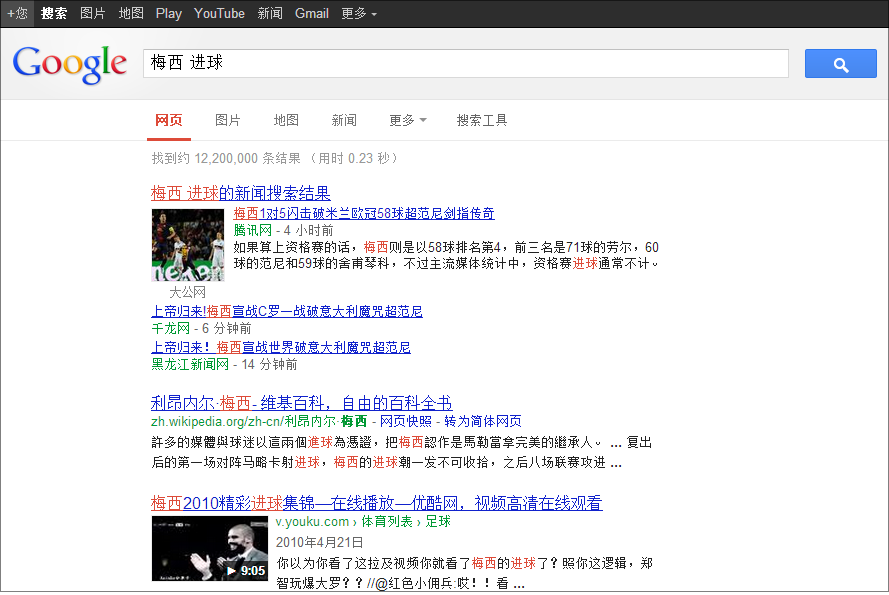
\includegraphics[width=5in]{queryExample.png} 
	\caption{基于关键词搜索结果}\label{fig:queryExample} 
	\end{figure} 
   
	搜索的目的在于获取知识,自然语言是表达知识的一种形式,却不是唯一的形式。在计算机技术中,自然语言是不容易被理解的,人们就提出了用本体来表达知识的方式,本体也成为了现代语义网的支柱。
   
	本体(Ontology)最初是一个哲学概念,后来被引入到计算机技术中,Neches等人最先定义了本体,即“给出构成相关领域词汇的基本术语和关系,以及利用这些术语和关系构成的规定这些词汇外延的规则的定义。”\cite{3}本体优势在于其精确的描述,可以摆脱语言层面的干扰,而真正上升到概念层面进行描述,为语义搜索提供基础,通过推理机,也能把隐性知识转换成显性知识。比如,“汤姆是一只猫”,就可以推理出“汤姆是一个动物”,以此为基础,不仅可以检索到汤姆作为一只猫的特征,也可以检索到汤姆作为一个动物的特征。这种基于本体的语义性搜索,就可以给用户提供更多的有用信息。
   
	对搜索性能的评估,主要有两个参数——查全率(Recall)和查准率(Precision),查全率用来衡量搜索系统查找相关文档的能力;而查准率用来衡量搜索系统过滤非相关文档的能力。\cite{4}显然,基于本体的语义性搜索,可以规避词语可能出现的歧义,通过推理机,合理拓展搜索范围,从而有效提高搜索的查准率和查全率。现在,也存在SPARQL等查询语言,可以实现精确的语义网搜索,但是它有一套复杂的语法,要求终端用户具有本体等多方面的知识,并不能真正的提高搜索效率。

	针对上述问题,本项目拟以机械领域为例,建立一种基于本体的语义性搜索系统。使得用户可以像常规方式那样输入关键词,系统首先用本体对关键词进行语义解析和扩展,再在语料库中进行搜索,给用户提供丰富而精确的查询结果。
	\subsection{发展现状}
	对于基于本体的语义性搜索系统,需要对本体和语义性搜索两个方面进行研究。
		\subsubsection{本体}
	根据应用范围的不同,本体可分为领域本体、通用本体、应用本体等。领域本体指在特定类型领域或某个学科的相关知识组成的本体。通用本体则涵盖若干个领域。应用本体包含某个特定领域的设计知识。
	
	Fabian M. Suchanek\cite{5}等人介绍了YAGO本体,它从维基百科和语义网上获得知识,涵盖面广,信息准确,还提供了强大的查询接口,是一种被广泛运用的通用本体。
	
	Ashburner\cite{6}等人建立了生物过程、分子功能、细胞组成三个本体,组成基因联合本体,生成了一套用于真核生物的动态可控的词库,同时扩展了细胞中基因和蛋白质功能增加和变化的知识,还建立了网站(http://www.geneontology.org),提供搜索接口,是领域本体与搜索结合的,应用于实际研究的例子。
	
	Maedche\cite{7}等人提出了一种本体学习框架,通过半自动的本体构建工具搭建典型的本体工作环境,通过本体导入、提取、修剪、提纯、评估等步骤进行建模,同时提出了用自由文本、字典等非结构文本进行本体构建的方法。
	
	Deborah L. McGuinness\cite{8}等人介绍了OWL语言,比较其与XML,RDF,RDF Schema(RDF-S)的差异,阐释为什么要采用OWL语言进行本体描述,并分别介绍了OWL三种子语言:Owl Lite,OWL DL,OWL FULL的联系与区别。为最后选择本体描述方法提供指导。
	
	上海交大王英林\cite{9}等人提出基于本体、知识处理模块与基于实例推理方法的可重构知识管理系统框架,实现了知识类型扩充的功能,讨论了基于工作流程的协作知识生产方法。
	
	中科院数学研究所金芝\cite{10}等人开发了一套基于本体的需求自动获取方法,该方法以企业本体和领域本体为线索来描述现系统,重用领域需求模型以构造应用软件需求模型,是本体的另一种运用方法。
	
	中国科学院文献情报中心李景\cite{11}等对构建知识本体的方法体系进行了比较研究,阐述了当前常用的7种知识本体构建方法,分别探讨它们的优缺点。
	
		\subsubsection{语义性搜索}
	Sara Cohen\cite{12}研发了一种面向XML的语义性搜索系统,支持用简易的检索语言进行搜索,并用扩展信息检索系统将查询结果进行排序,输出与查询相关的文档块。

	Thanh Tran\cite{13}等人提出一种基于本体的语义性搜索方法,其核心在于用本体将搜索关键词转换成为查询语言,这种方法可以用于浏览声明过的知识,完成一些语义搜索,但是之后的评估表明这种方法存在一定的局限性。

	基于上述的方法,Qi Zhou\cite{14}等人开发出一套“Spark”系统,将关键词翻译成正式的逻辑查询,使得用户可以用熟悉的关键字搜索实现语义搜索的功能。

	Li Ding\cite{15}等人开发了一套基于爬虫索引的语义网搜索系统“Swoogle”,其工作方法是将找到文档的元数据抽取出来,计算出文章之间的关系,再以URI作为索引关键字来查找相关文章。

	METU的Soner Kara\cite{16}等人运用语义性索引,提出了一种基于本体的检索系统。先用爬虫程序获得数据,将本体实例化,通过信息抽取和推理得到完全的实例关系OWL(Ontology Web Language),再转换成索引进行搜索。并把它应用于足球领域,拥有较好的搜索性能。

	Sugato Chakrabarty\cite{17}等人通过建立同义词表,一定程度上解决了类似缩写与全称的同义词关系,提高了查全率,并成功运用在了通用汽车公司的维修查询系统中。

	普渡大学的Zhanjun Li\cite{18}等人提出了一种框架,采用本体基础和算法来处理复杂查询,通过计算相关度,在一词多义的情况下,准确判断出用户的真实意图。

	台湾大学的Hsien-Tang Lin\cite{19}等人设计了一种方法,通过领域知识,把文章化分为段落,再把每个段落作为一篇独立的文章,解决了对于较长文章有多个主题,不便于进行处理的问题。

	浙江大学的胡玥姮用PLIB本体和XML技术对制造信息进行结构化描述,建立描述网页内容混合向量空间模型,设计了对零件资源信息的概念搜索系统。

	中国人民大学的Anjian Ren\cite{20}等人利用现成的YAGO本体,针对用户的具体查询,自动生成合适的分类,克服了在搜索关键字过于笼统时,搜索结果不理想的问题。

	上海交大的Dong Yang\cite{21}等人,用基于本体的方法,开发出一套可以自动进行产品配置系统,以同时满足客户需求和技术指标。

	浙江大学郭剑锋\cite{22}等人建立了零件库本体,并实现了关键字扩展搜索。

	综上所述,现在基于本体的语义性搜索是研究的热点问题,国内外研究取得了一些成果,但是也存在很多问题。首先,在需要大量设计知识的机械设计领域,并没有构建出一个较完整的本体,谷歌等通用的搜索工具又不便于搜索出专业性较强的设计知识。其次,没有提出一种扩展性较好的方法框架,文献\cite{15}中提到了其方法具有较好的可扩展性,但是其前提是所涉及领域模板简单。本项目以较为庞大的机械设计领域为例,开发出一套具有较高可扩展性,可移植性的基于本体的语义性搜索系统。
		
	\subsection{论文主要研究内容}
	本项目拟通过本体描述机械设计知识,基于本体组织语料库,形成以本体为骨架、语料库为内容的机械设计领域的知识库。再利用本体的扩展和推理功能, 真正从语义层面理解用户的查询要求,通过一定的搜索算法,在知识库中搜索出相关度较高的条目作为搜索结果。
	
	系统开发流程:首先,构建机械设计本体作为搜索系统的核心;然后,探究如何运用本体进行知识的推理和语义的扩展,建立扩展性语义搜索算法;接下来,用爬虫程序获得模拟语料库,用本体重新组织语料库,从而获得搜索的知识库;最后,将以上几个部分结合在一起,增加用户接口,完成搜索系统的搭建。

	本文以机械产品设计为背景,设计并开发了一种机械设计知识搜索引擎系统,并针对其中的若干关键技术进行了深入研究。具体研究工作包括:
	\begin{enumerate}
		\item
	
	研究知识的表达和存储方式,研究本体构建技术,扩展和推理功能。以本体描述机械设计知识,从而实现自然语言和搜索系统的联系。研究本体建模理论,构建机械设计的基础本体,确定本体建模工具。正确使用类,个体,对象属性,数据属性等建模类型,建立恰当的继承关系,关系特性(即函数关系,反函数关系,对称关系,反对称关系,传递性等)及对象的逆特性,从而为后面的推理过程提供基础。采用基于Web本体描述语言(OWL)的形式化描述语言,方便之后步骤中对于本体的调用。研究类层与个体层的关系,为后续本体的扩展提供支持,为在搜索时进行合理的关键词扩展提供方便。
		\item
	研究可以实现语义扩展功能的、具有设置参数接口的搜索算法,并提出一种评分和排序方式,使得排序靠前的结果更可能是用户最想要得到的结果,达到捕捉用号意图的目的。
		\item
	研究Web应用系统的相关常用技术,包括搭建服务器,数据库技术,前端设计等。为保证搜索系统的跨平台通用性和可扩展性,将其定位为Web应用,采用B/S(Browser/Server)架构,而不是C/S(Client/Server)架构,这样就不用在客户端安装专用搜索软件,只需在浏览器中,像进入普通网页那样,就可以实现搜索,大大提高了搜索的便捷性,这也就需要架设服务器,通过数据库来管理维护知识库,并且编写友好的用户界面,方便用户使用。
		\item
	研究知识库建立的方法,通过爬虫程序,在维基百科上获得与机械相关词条网页,对其进行解析,去掉HTML标签,获得非结构化的文本信息,模拟语料库,以关系数据库的方式进行存储。研究关系数据库与本体之间建立的关系,以本体为骨架,数据库为内容,重新组织数据库,以提高搜索效率。
		\item
	设计并开发一种基于本体的、具有语义扩展功能的搜索引擎基础架构,提供灵活的参数设置接口和底层数据更新接口,为知识检索提供一种高效的方式。在理论和方法研究的基础上,集成各功能模块,增加用户操作界面,研究各模块之间信息交流,相互调用的方式。使得各模块具有自己较为独立的功能,以实现之后对于其他领域应用的扩展,松散耦合地集成模块,并将此架构运用于机械领域,开发出捕捉查询意图的机械领域知识检索系统,并进行性能验证。
	\end{enumerate}

	\subsection{论文结构}
	论文后续部分将围绕捕捉查询意图的机械领域知识检索系统的设计开发以及其中关键的技术研究展开。具体的安排如下:

	第一章介绍论文的研究背景和研究意义,阐释具有语义扩展性功能的、可以捕捉查询意图的搜索系统的重要性,并对相关技术的研究现状进行了介绍。最后,给出了论文的研究内容和组织结构。

	第二章介绍捕捉查询意图的知识检索系统的总体设计,通过介绍现有搜索引擎技术,提出功能扩展的方法,建立系统体系结构图,从而引出系统中包含的若干关键技术,为后续章节中相关关键技术的阐述提供系统背景。

	第三章介绍知识的表达方式,引出本体,介绍本体的基本属性和构建方法,利用本体的推理功能,实现隐性知识到显性知识的过渡,实现语义的扩展。介绍本体的存储方式,并介绍操作本体的Java工具包——Jena。最后介绍了一种建立本体的软件——Prot{\'e}g{\'e}。

	第四章首先介绍扩展性语义搜索算法的其本原理及定性的排序方式,然后介绍Java工具包——Lucene及其功能实现的方式,接下来阐述排序的定量依据,最后介绍对搜索系统性能的评价指标。

	第五章介绍其他在系统实施阶段所涉及的技术,这些技术也是开发Web应用的基本技术,包括数据库技术,搭建服务器,以及前端UI编写。最后介绍B/S架构的优势及其在系统中的应用。

	第六章在前几章对体系结构和关键技术介绍的基础上,以软件工程的思路,从需求分析、概要设计、详细设计,三个层面进行分析和阐述,介绍搜索系统是如何实现的。最后展示系统使用全貌,并进行系统的性能测试。

	第七章总结全文,并对系统未来的改善进行展望。
\newpage	
\section{系统总体设计}
%初始化编号
\setcounter{figure}{0}
\setcounter{table}{0}
\setcounter{equation}{0}
	本章首先对普通搜索引擎的核心和机制进行介绍,以此为基础框架,扩展出本项目的检索系统的大致框架。进行系统整体设计,探讨知识表达的技术并确定知识表达的方法,构建系统体系结构。最后梳理其中涉及的关键技术,包括本体的构建和扩展性主义搜索算法。
	\subsection{搜索引擎简介}
	要了解搜索引擎,首先需要了解信息检索技术。信息检索(Information retrieval,IR)是指从大规模电子文本(通常存储在计算机上)找出满足信息检索要求的非结构化的自然语言数据(通常是文本)。\cite{23}
	
	信息检索技术的应用已经非常普遍,几乎所有与网络有关系的人,都会或多或少地使用该技术。目前,Google和Bing,国内的百度,作为一种Web搜索引擎,已经让信息检索技术深入寻常百姓家,成为目前为止最普遍和大量使用的信息检索服务的形式。与此同时,电子图书馆中检索期刊文章和会议报告,大型企业中利用企业搜索系统来管理和查询电子邮件、备忘录、技术报告和其他业务文档,也是信息检索就用的突出体现。
	
	由此,可以看出搜索引擎是信息检索的一种具体应用,而信息检索技术是搜索引擎的核心。
		\subsubsection{搜索引擎本质}
	搜索引擎的核心是信息检索技术,检索模型提供了一种度量查询和文档之间相似度的方法。\nocite{24} 文献\cite{25}对搜索引擎进行了数学表述:通过一定结构维护文档集M,定义一个相关性函数SC(Similarity Coefficient),其满足:
	\begin{equation}\label{eq:1}
	 SC: D \times Q \longrightarrow \mathbb{R}
	\end{equation}
	
	其中D代表文档集,Q代表用户的所有可能检索请求集合,R代表实数集合。当用户给定一个检索请求q时,搜索引擎的目标是利用相关性函数SC为D中的文本打分,从而在文档集D中找到一个k元素的有序的文档序列T:
	\begin{equation}
	T=\{ m_{1},m_{2},m_{3},\cdots, m_{k} \},\forall m \in T 且 n \in \bar{T} 满足 SC(q,m)>SC(q,n)
	\end{equation}
	
	即查询结果的文本序列T中的文本总是比那些序列之外的文本得分要高。
	
	与此同时,在文本的内部,也满足:
	\begin{equation}
	\forall i < j, SC(q,m_{i})>SC(q,m_{j})
	\end{equation}
	
	即排在前面的文档(编号较小)得分总比排在后面的文档高。
	
	由此,搜索系统的根本归结在了建立式\ref{eq:1}中的相关性函数,即检索模型。
		\subsubsection{检索模型}
	常用的检索模型有如下几种:
	\begin{itemize}
		\item
	布尔模型:原始的布尔模型通过查询与文档的简单比对,判断出二者相同或不相同,相当于相似度只有无穷和零两种情况,没有相似度的考量,是最原始最朴素的模型,之后,通过对查询词条加进权重,给出了一种可以进行相关性排序的算法。\cite{salton1970}
		\item
	向量空间模型:将查询和文档表示为词项空间中的向量,判断相似度的传统方法是计算两个向量的内积,计算其余弦相似度,以此反映查询与文档的相似度。\cite{salton1975}之后,通过引入不同文档集的权重,提出了TF-IDF(词频-文档逆向频率)\cite{robertson1976}来表达相似度的模型。
		\item
	概率模型:把相似度问题降为概率论应用的问题,通过计算文档与查询相关的概率,来表示文档和查询的相似度。
		\item
	语言模型:用文档中词的概率分布,为每一个文本建立一个语言模型,然后通过伯努利事件进行建模, 以条件概率来表达文档和查询的相似度。\cite{ponte1998}
	\end{itemize}
	
	此外,较常用的检索模型还有推理网络、LSI(隐性语言检索)、神经网络方法、遗传算法、模糊集检索等模型,此处不再赘述。
		
		\subsubsection{搜索引擎基本架构}
	一个常规的搜索流程如图\ref{fig:basicStructure},通过爬虫程序,从互联网上获得文本,构成原始资料库,以此建立索引库和有序资料库,搜索引擎的用户在文本框里输入一个简单的查询(query),它可能包含几个词项(term),通过索引库的逆排索引(inverted index)获得相关搜索结果在有序资料库中的位置,然后将结果显示给用户。
		
	\begin{figure}[htbp] 
	\centering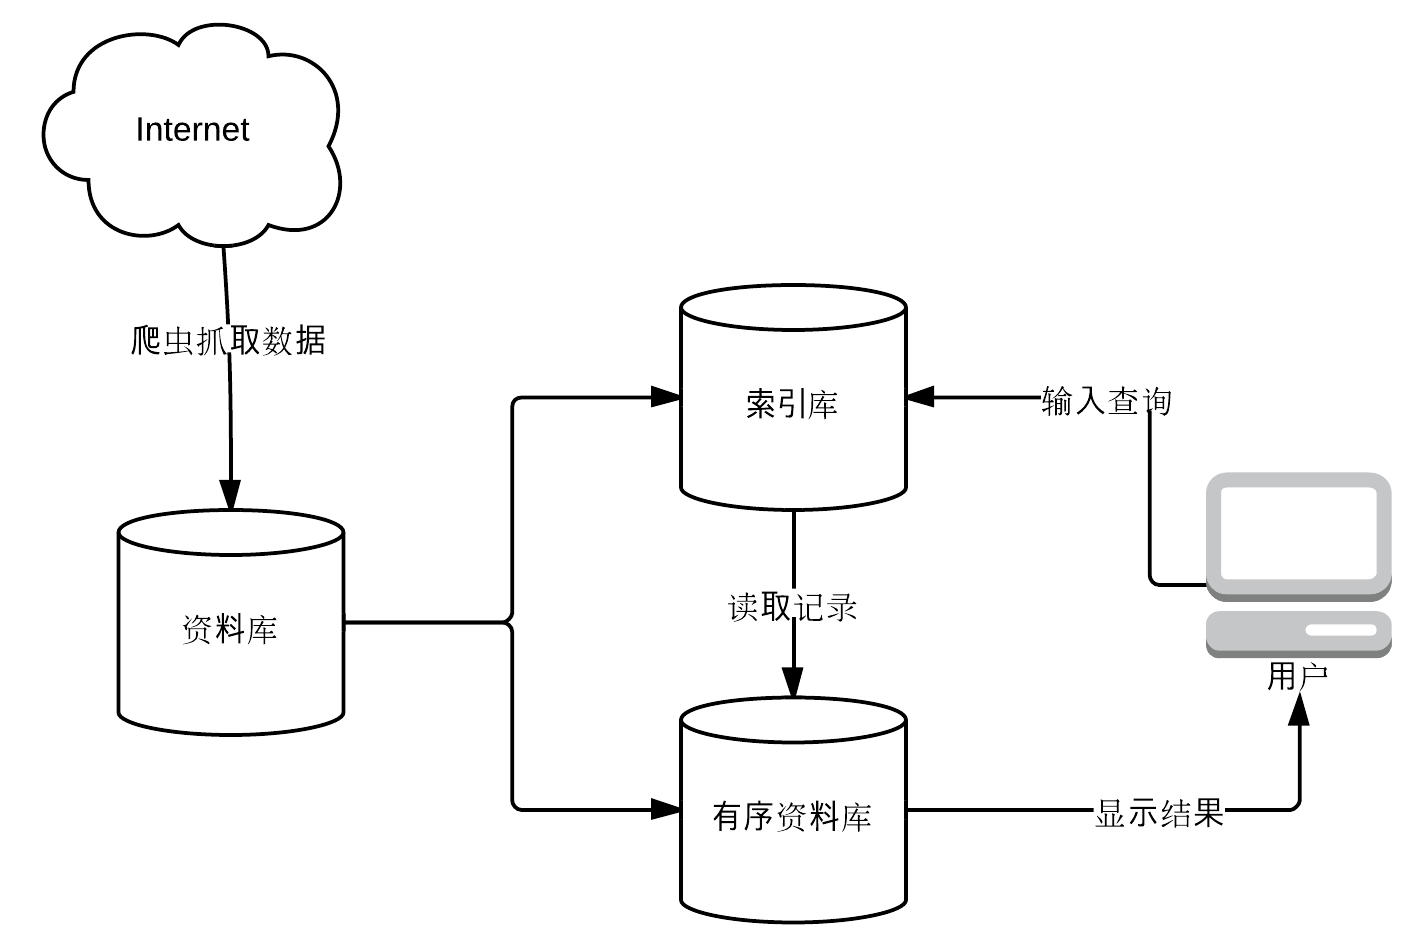
\includegraphics[width=5in]{fig/basicStructure.png} 
	\caption{搜索引擎基本架构}\label{fig:basicStructure} 
	\end{figure} 
		
	\subsection{总体设计}
		\subsubsection{知识的表达}
	知识是人们在社会实践活动中所获得的认识和经验的总和。具体地说,知识是人们对客观世界的规律性的认识。\cite{Chen2010}
	
	在漫长的人类文明中,人类积累了丰富的知识,它们被以文字、图表、声音、图像等形式记录下来,但是对它们的高效重用,仍然是制约发展的重要因素。以机械设计为例,众所周知,该领域的经验比知识更重要,但是经验的积累是从实践中逐步内化的,需要漫长的时间,有的经验以文字的形式记录下来,在重用的时候却发现检索的成本太高,这就造成了经验层面的知识无法进行较直接的高效的传承。
	
	随着信息技术的发展,知识工程、人工智能等新兴的领域也取得了日新月异的进步,它们研究的核心之一就是高效地存储、获取和使用知识。机械设计知识的检索也是一种知识检索的形式,在此,有必要就人工智能中知识的分类和表达进行简要的介绍。知识大致可以分为以下几类:
	\begin{itemize}
		\item
	事实性知识:陈述客观性的知识,比如齿轮机构可以传递力和运动。事实性知识一般采用直接表示的形式。
		\item
	过程性知识:描述做某件事的流程,比如轴的加工工序。
		\item
	规则性知识:亦称产生式规则(Production Rule),规则性知识由两部分构成,一部分是前提,另一部分是结果,用逻辑关系"IF THEN"来描述。
		\item
	启发式知识:对解决问题有帮助的经验法则或技术,这种知识在描述上较为困难,有效性和效率都有待于研究,是人工智能的主要课题之一。
		\item
	实例性知识:包括已经形成的大批观察数据和案例,关于事物的知识都隐蔽在实例之中,这不是直接的知识,确实其他类型知识的重要来源。
		\item
	元知识:即所谓关于知识的知识,它告诉系统如何利用系统内部存储的知识,指导了系统运行和推理。
	\end{itemize}
	
	由此可以看出,本搜索系统的功能之一,就是要得利用元知识将隐蔽在实例性知识中的其他知识挖掘并呈现出来。
	
	人类的交流是基于自然语言的,要实现人机的交流,就需要将自然语言表述的知识转化成计算机可以使用的。这就涉及到知识表示(Representation of Knowledge)问题,现在成功运用的知识表示形式主要包括:数理逻辑,产生式规则,语义网络,框架,剧本,本体,下面就此进行简要介绍。
	
	数理逻辑是用逻辑符号语言进行精确的,没有歧义的描述,用数学方法进行研究;产生式规则表示为“if A then B”,即如果A则B,以此可以实现正、反两种推理;语义网络是用网络的形式,用弧连接概念,这样就把概念和它们的关系转换成了一张结构图;框架由框架、槽(属性)、侧面、值组成,一个槽可包含若干侧面,一个槽对应一个值,这样就形成了对于知识的树状描述;剧本描述了事件的起因、因果及事件间的关系,便于描述业务流程。本体定义了公共词汇集,把现实社会中某个应用领域抽象成概念及概念间的关系,以此来实现信息共享和知识共享。 
	
	本系统采用本体来描述知识,并以此实现语义扩展,隐性知识向显性知识转换的功能。下面就对本体作介绍。
	
	本体最初是一个哲学概念,是指关于存在及其本质和规律的学说,在哲学中记作本体论(Ontology)。后被引入到计算机技术中,用以概括概念及它们之间的关系,记作本体(ontology)。在1993年,Gruber定义了本体——“本体是概念化(Conceptualization)的一个显示的(Explicit)规范说明或表示。”\cite{gruber1993} 在一些简单情况下,本体只是概念的分类层次结构,就像植物学、动物学分类,领域本体以概念树的方式,将概念进行分类,如图\ref{fig:生物分类}。
	
	\begin{figure}[htbp] 
	\centering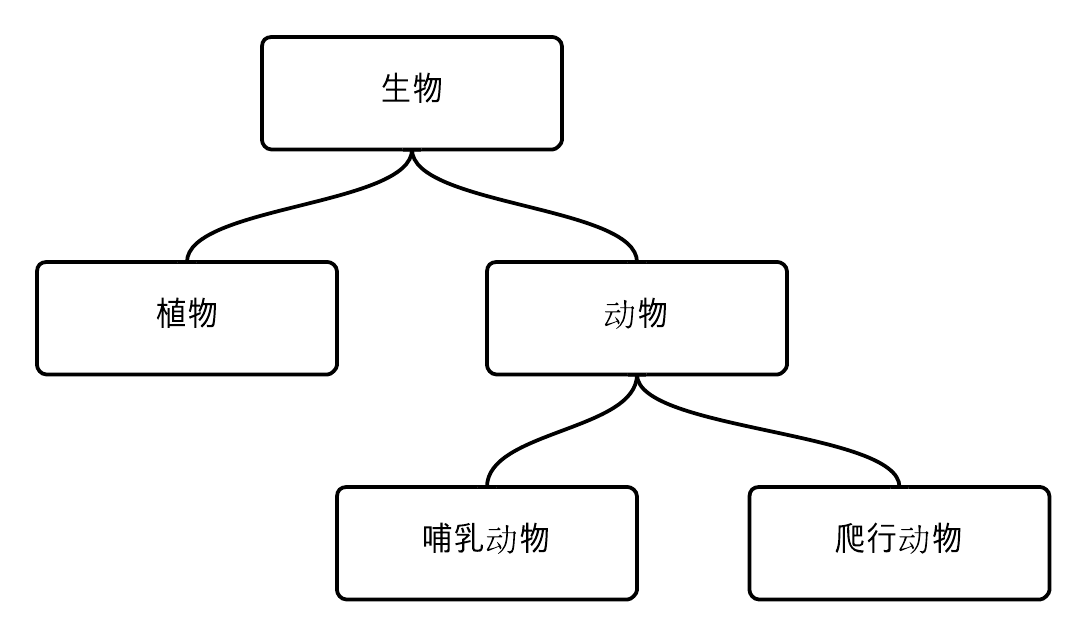
\includegraphics[width=3in]{fig/biotax.png} 
	\caption{生物分类图}\label{fig:生物分类} 
	\end{figure}	
	
	但是这样简单的树状结构是难以描绘真实情况的,比如,针对一个直齿圆柱齿轮,从分类上说,它是齿轮的一种,所以应该是是齿轮的子结点,但是对一个装配体,在其装配树结构中,齿轮可能又是一个变速箱的子结点。所以,作为一个描述知识的方式,概念树就太过简单了,所以在复杂情况下,本体并不是简单的概念树,而是又加入了关系、公理、规则。
	
	一个完整的本体包括5类基本元素:概念、关系、函数、公理、实例。即:$O::=\{C,R,F,A,I\}$。\cite{Chen2010}
	
	C:概念(concept),除一般意义的概念外,还拓展到任务、功能等。
	
	R:关系(relationship),描述概念之间的关系,比如“subclass-of”(子类),可以表示一个概念继承了另一个概念。关系可以表述为$ R:C_{1} \times C_{2} \times \cdots \times C_{n} $, 即$C_{1}、C_{2}、\cdots 、C_{n}$之间存在n元关系。
	
	F:函数(function),即某个元素$C_{a}$可以由其他元素$ \{C_{i}\} $唯一确定,比如对于一个圆形,知道其半径,就可确定其面积。
	
	A:公理(axiom),概念或关系所满足的永真式,比如一个子类继承其父类的特征。
	
	I:实例(instance),概念类所对应的具体实体。
	\\
	
	当然,关于本体,到目前为止仍没有明确的数学定义,所以对于上述元素,在实际应用中,可能还根据需要进行设计。在后续部分将会做阐述。
	
	本体优势在于其精确的描述,可以摆脱语言层面的干扰,而真正上升到概念层面进行描述,为语义搜索提供基础。通过推理机,也能把隐性知识转换成显性知识。比如,“汤姆是一只猫”,就可以推理出“汤姆是一个动物”,以此为基础,不仅可以检索到汤姆作为一只猫的特征,也可以检索到汤姆作为一个动物的特征。这种基于本体的语义性搜索,就可以给用户提供更多的有用信息。

		\subsubsection{系统体系结构}
	本文设计并开发了捕捉查询意图的机械领域知识检索系统,以此进行机械知识的快速查找。作为搜索引擎的一种,本系统具有与经典搜索引擎相似的体系结构,但是由于从本档库组织、搜索方法等方面都有其特殊性,所以同一般网页网页搜索引擎相比,本系统又有其特殊之处,下面介绍捕捉查询意图的机械领域知识检索系统的体系结构。
	
	本系统体系结构如图\ref{fig:体系结构},系统自下而上分为资源层,应用服务层,表示层,客户端层。
	
	\begin{figure}[htbp] 
	\centering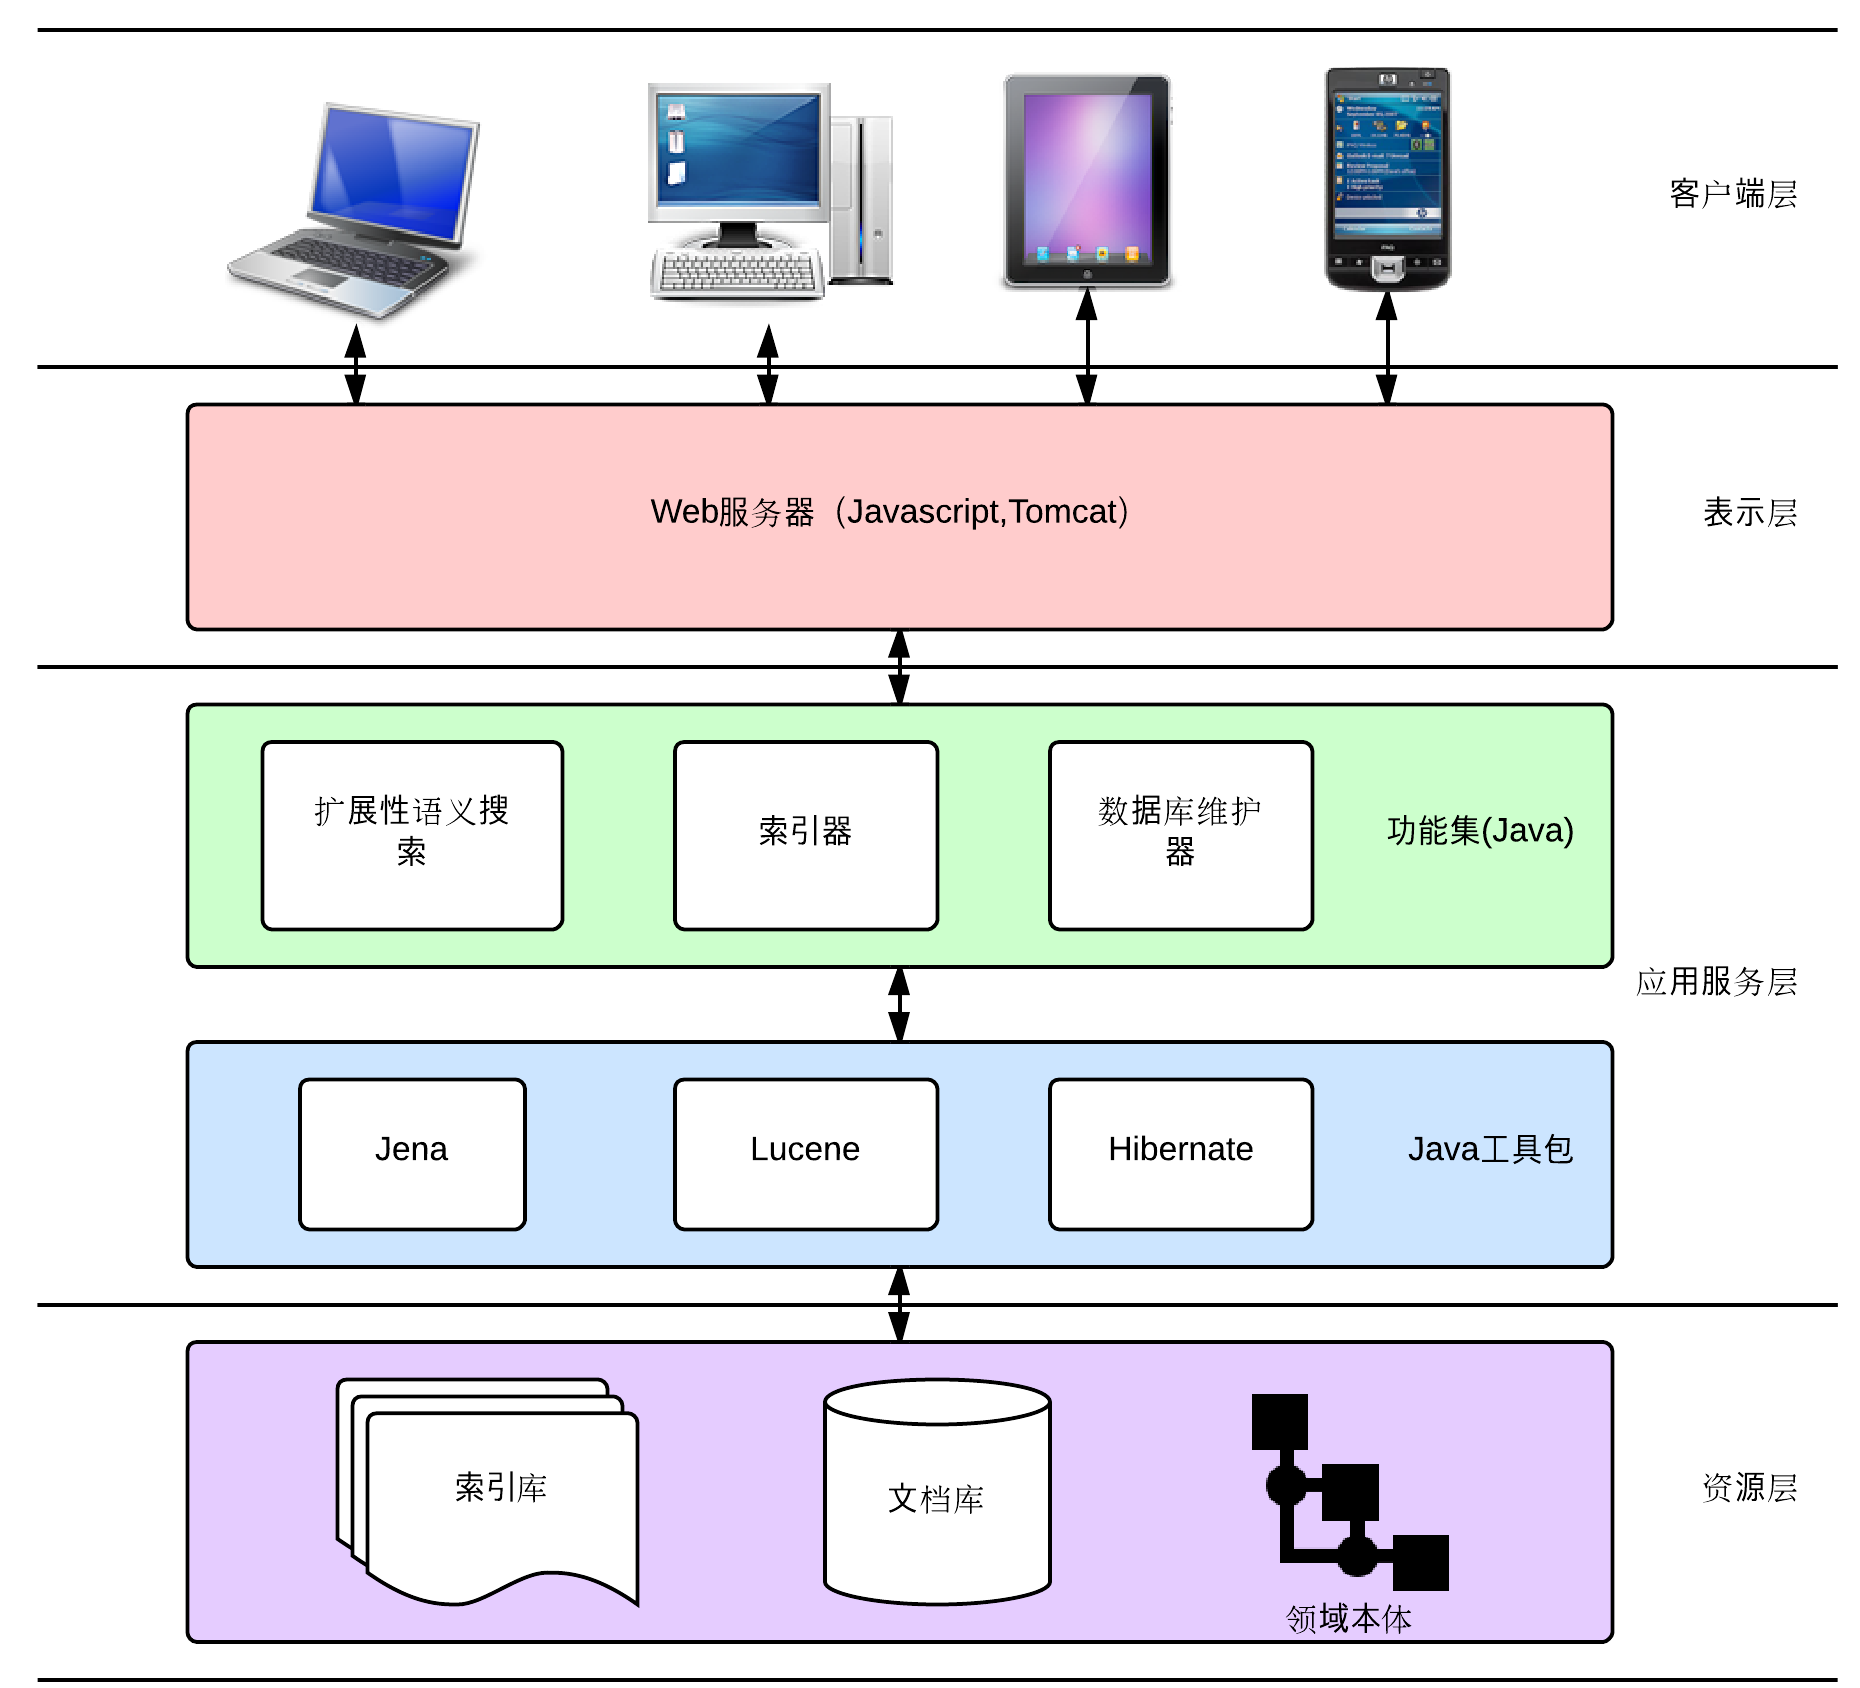
\includegraphics[width=4in]{fig/SystemStructure.png} 
	\caption{系统体系结构图}\label{fig:体系结构} 
	\end{figure} 
	
	\begin{itemize}
	 	\item
	资源层:资源层为检索系统提供了有组织的文档库,它是通过爬早程序从互联网上获得的文档,通过解析操作,去掉了HTML标签,转化为非结构化文本,将其组织在数据库中,作为被搜索的文本;提供了领域本体,本体的建立结合了人的认识规律,按照本科教学的学习培养方案,将《机械原理教程》《机械设计教程》进行一定的简化和概括,再按照一定的本体构建规则,以本体形式录入,作为扩展性语义搜索算法的基础;提供了本体的实例层,为实例搜索提供数据源,同时,由于本体的推理功能是在实例层进行的,所以为实现推理功能,而不是单纯的扩展功能,需要将一些重要概念进行实例化,从而更好地利用了本体的另一强大功能。
		\item
	应用服务层:应用服务层主要包括两个部分:
	
	Java工具包层,提供Jena、Lucene、Hibernate等工具包,Jena实现了本体的读取操作、Lucene实现文档库索引与搜索功能、Hibernate实现操作数据库的功能。这些工具包强大而灵活,为系统开发提供了极大的便利,缩短了开发周期。该层也是连接应用服务层与资源层的枢纽层。
	
	功能集层:这是检索系统的核心部分,提供扩展性语义搜索功能,索引器功能和数据库维护器功能。索引器可以对特定目录的文档创建索引,数据库维护器可以把这些文档加入到搜索数据库中,从而实现了知识库维护功能,将本体、知识库、扩展性语义搜索算法松散耦合地集成在一起,同时提供灵活丰富的接口,保证与表示层的正常通讯,同时为今后功能扩展提供支持。
		\item
	表示层:在表示层内采用开源的Tomcat容器架设服务器,采用B/S架构,在服务器端完成大部分业务逻辑,减轻客户端负载。采用Javascript和ExtJS库编写用户界面,可以相对容易地实现美观友好的用户界面,使用户便于使用系统提供的功能集。这样,就保证了系统的跨平台性。
		\item
	客户端层:客户端层为用户终端,由于系统采用了B/S架构,用户无需安装客户端软件,只需像登录普通网页那样,登录检索系统网页,就可以使用系统各项功能。系统逻辑主要由部署在服务器端的程序完成,这样也就使对客户端层的设备配置要求低,保证了系统的跨平台性。由于对移动平台的兼容性,可以让设计人员在任何时候都能方便地查询所需要的设计知识,符合了“随时随地设计”的理念。
	
	\end{itemize}
	
	系统工作功能框图如图\ref{fig:功能框图}。
	
	\begin{figure}[htbp] 
	\centering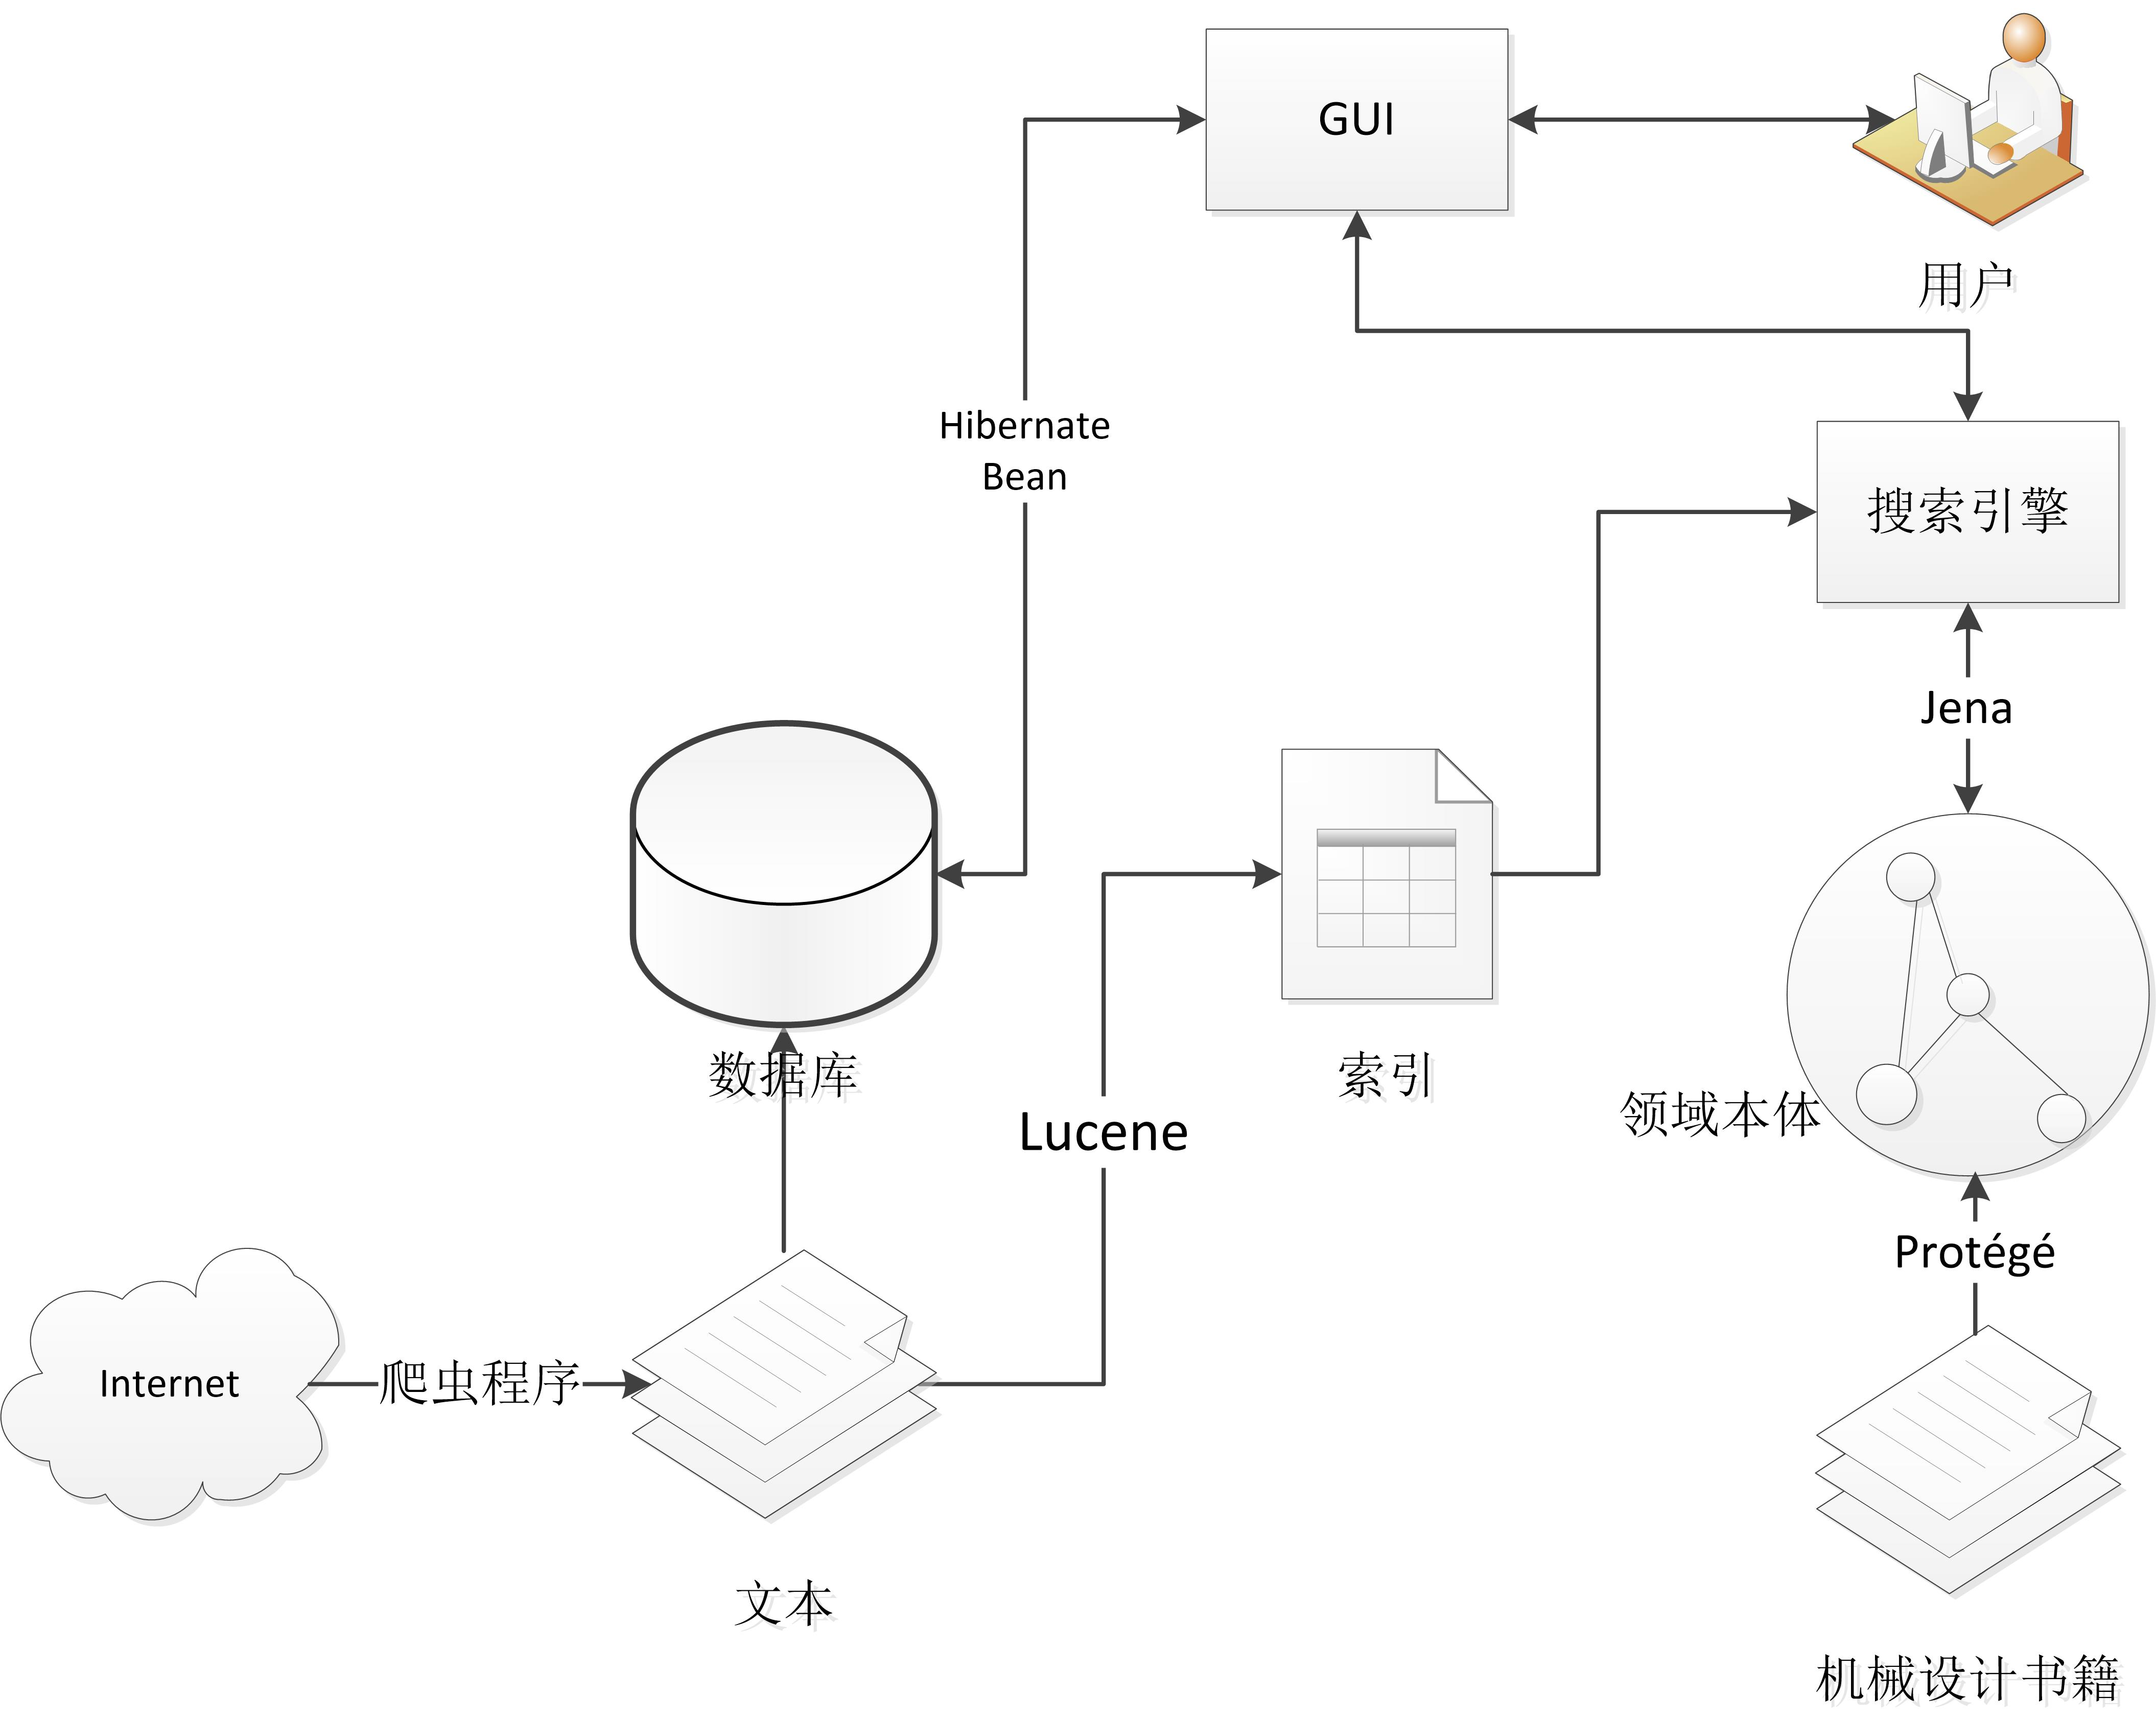
\includegraphics[width=4in]{fig/功能框图.jpg} 
	\caption{系统工作功能框图}\label{fig:功能框图} 
	\end{figure} 
	
	通过抽象机械设计书籍中的概念,用Prot{\'e}g{\'e}建立领域本体;通过爬虫程序,从互联网上获得领域相关的文本,将这些文本录入到数据库中,同时通过Lucene建立文本索引。搜索引擎可以通过Lucene调用索引,通过Jena 调用领域本体,当用户有查询请求时,通过用户界面将查询传到搜索引擎中,进行搜索,获得结果ID,从数据库中获得对应ID的文本,在用户界面中呈现出来,完成搜索流程。
				
	\subsection{关键技术分析}
		\subsubsection{本体的构建}
	根据搜索系统要求,利用本体主要完成两方面的任务:
	\begin{enumerate}
		\item
		实现语义的扩展
		\item
		实现知识的推理
	\end{enumerate}
	结合这样的要求,拟定本体构建的大致思路如下:
	
	首先,针对机械设计领域的知识,将概念化分为三大类(Prot{\'e}g{\'e}中称作Class):object(对象),function(功能),feature(特征)。对象包括机构、构件、运动副、零件等客观存在的实体;功能就表示机构、零件等对象可以实现的功能,比如齿轮机构可以改变转速,改变转速就是一种功能;特征则描述对象的基本特征,形状特征定义了诸如分度圆等可以描述零件尺寸的特征,物理量特征则对形特征(比如分度圆直径)和功能(比如传动比)进行定量描述。这样,就可以建立出粗略的树状结构的领域本体,并且可以直接采用它们的继承和被继承的关系。
	
	然后,在以上一步建立的树状本体基础上,添加关系(Prot{\'e}g{\'e}中称作对象属性(Object Property)。与上述三类概念对应,将关系也分成三类:“具有对象”,“具有功能”,“具有特征”,这样就可以沟通上述三大类概念。比如建立“具有功能”关系,将齿轮机构与传递功能相联系。这样一来,就把概念树扩展成为了一个有向图$ G=(C, R) $,从而为实现语义扩展提供基础。
	
	接下来,建立上一步中建立的关系的函数特性。在Prot{\'e}g{\'e}中,这些特性(Characteristic)包括函数关系、反函数关系、对称关系、反对称关系、传递关系等,这些关系将在后文进行介绍。通过这些关系,实现推理功能,将潜在的关系挖掘出来,将隐性知识转换成显性知识,得到一张扩展有向图$ G'=(C, R')$,它能使语义获得更丰富的扩展。
	
	最后,根据需要,再建立相应的实例,完成本体的构建。
	
		\subsubsection{扩展性语义搜索算法}
	通过本体的构建,可以获得一张表述概念及概念关系(包括显性的和隐性的)图$ G'=(C, R') $,下面就要建立一种算法来实现语义的扩展搜索算法。在目前暂时不考虑搜索的时间复杂度的情况下,搜索算法可以归结为之前所提到的式\ref{eq:1}中的相关性函数,即一种对搜索结果的打分机制。按照这样的想法,拟定搜索算法流程,如图\ref{fig:搜索算法流程}。
	
	\begin{figure}[htbp] 
	\centering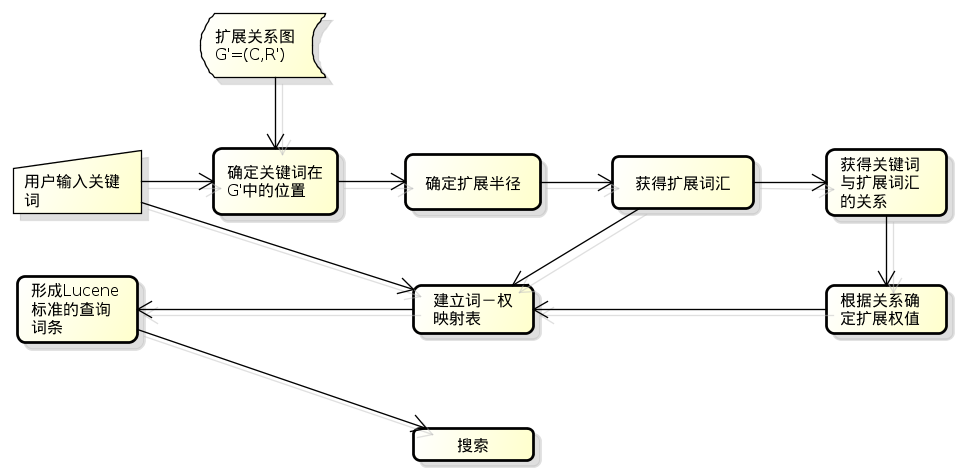
\includegraphics[width=5in]{fig/searchFlow.png} 
	\caption{搜索算法流程}\label{fig:搜索算法流程} 
	\end{figure} 
	
	首先,用户输入一个关键词t,系统读取图G',确定了t在G'中的位置,根据搜索半径r,确定与关键词t相关的概念$\{c\}$,然后获得t与$\{c\}$中各关键词$c_{i}$的关系$R_{ti}$,在一个可修改的权值配置文件中,定义了不同类型的关系R对应的权值,这样就可以建立一张关于词-权的映射表,再通过这张表,生成能够被Lucene读取的搜索词条,最后进行搜索。
	
	Lucene中的加权搜索评分机制将会在后文进行介绍。这样就实现了具有权值配置功能的扩展性语义搜索算法。

\newpage
\section{本体的构建}
\setcounter{figure}{0}
\setcounter{table}{0}
\setcounter{equation}{0}
	本章具体介绍本体构建的实施步骤,具体介绍了采用Prot{\'e}g{\'e}软件进行本体概念树建立、概念关系的添加、关系特征的描述的方法,通过阐述关系特性的性质,说明本体实现推理的机理。接下来,介绍本体的存储方式以及用Jena包对本体进行读写操作的方法。最后对本体建模采用的软件Prot{\'e}g{\'e}进行简单介绍。

	\subsection{准备知识}
	本体是一种形式,它可以用不同的语言来表述,不同的语言提供了不同的功能。OWL(Ontology Web Language)是由W3C组织(World Wide Web)提出的一种描述本体的语言。在OWL中,有三种元素:类(Class),属性(Property),个体(Individual)。它可以近似地与之前提到的概念、关系、实例相对应。
		
	\subsection{建立本体的雏形}
	
	在Prot{\'e}g{\'e}中建立本体,首先面对的类的问题,类并不是孤立的概念,而是已经设定了子类(SubClass)和超类(SuperClass)等相关的概念并且设定了子类会继承其超类的属性。比如前文所提到的,汤姆是“猫”的一个个体,“猫”具有一个超类是“动物”,当描述了动物“具有眼睛”这样的属性,猫也会继承“具有眼睛”这样的属性。
	
	在建模的初始阶段,会遇到这样的问题。常见的从属关系有两种,一种是“is-a”,如图\ref{fig:“is-a”关系};一种是“part-of”,如图\ref{fig:“part-of”关系}。
	\begin{figure}[htbp]
	\begin{minipage}[t]{0.5\linewidth}
	\centering
	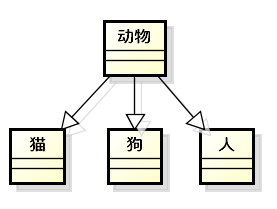
\includegraphics[scale=1]{fig/isA.png}
	\caption{“is-a”关系}
	\label{fig:“is-a”关系}
	\end{minipage}
	\begin{minipage}[t]{0.5\linewidth}
	\centering
	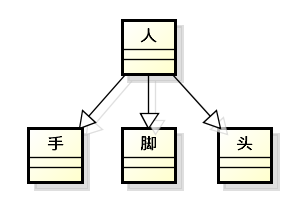
\includegraphics[scale=1]{fig/partOf.png}
	\caption{“part-of”关系}
	\label{fig:“part-of”关系}
	\end{minipage}
	\end{figure}
	
	“is-a”是本体组织的一种核心关系,用它可以描述出概念的三种关系:包含、相交、独立。
	
	若两个概念存在包含关系,则它们在“is-a”层次中处于上下层的父子关系;若两个概念存在相交关系,则它们在“is-a”层次中处于同一层的兄弟关系,即具有相同的父亲;若两个概念是独立的,则它们在“is-a“层次中没有直接的联系。
	
	容易混淆的一种情况是“part-of”,“part-of”表示了一种部分与整体的关系,就像机械领域中的产品结构树,管理领域的部分划分,都是一种树状的结构,但在建模时,如果误把这种关系当作类的结构,就会造成继承特性无法正常使用。比如,在图\ref{fig:“is-a”关系}所示的关系中,当给“动物”赋予有生命这一属性的时候,其子类“猫”、“狗”、“人”都继承了这一属性,易于理解,无论是人、狗、还是猫,都是具有生命的。但是如果误用了“part-of”结构,会发生什么事情呢?举个例子。在图\ref{fig:“part-of”关系}所示的关系中,如果给“人”赋予了“能说话”这样的属性,那么它的子类也会继承这样的属性,也就意味着“手”“能说话”,“脚”“能说话”,这显然是荒谬的。这也就解释了,在Prot{\'e}g{\'e}的类中,有一个根类“Thing”,因为无论是对象、或是特征,它们都应该是一种事物(Thing)。
	
	本体建立过程中,必须反复验证是否采用了“is-a”的方式进行类的组织,以确保可以正确使用继承关系。验证的方法就是在添加一个子类的时候,跟其父类作这样的一个判定“子类 是 父类 的一种吗?”比如,对于“齿轮”类,建立其子类“直齿圆柱齿轮”,容易判断,直齿圆柱齿轮是齿轮的一种,所以这个父子关系是正确的。但是对于“变速箱”类,“直齿圆柱齿轮”就不能是其子类,因为我们容易判断“直齿圆柱齿轮是变速箱的一种”这种表述是错误的。通过这样的方法,就能够建立起能够合理利用OWL中父子继承关系的本体。
	
	用这样的方法,建立起了本体的雏形,即一个粗略的树状结构的领域本体。对于一张本体图$ G=(C,R) $,现在就完成了C(概念)部分的建模。下面进行关系(R)层次的建模。
	
	\subsection{建立关系}
	在上一步中,建立了树状结构的领域本体,完成了本体的概念部分建模。通过树的结构,也进行了概念间父子继承关系建模,下面将完善关系层次的建模。
	
	在Prot{\'e}g{\'e}中,与OWL中的属性(Property)元素相对应的有三种:对象属性(Object Property),数据属性(Data Property),注释属性(Annotation Property)。在一个“主-谓-宾”三元描述中,属性都充当了谓语的功能。
	
	对象属性:根据Prot{\'e}g{\'e}提供的官方讲义,对象属性是用于描述个体关系的,但是在建模过程中,个体都不是孤立的,它们都依托于一些特定的类,所以对象属性可以借用来描述概念与概念之间的关系,此处的概念是指用户自己建立的类,也就是说,对象属性所连接的主语和宾语都是用户建立的概念。
	
	数据属性:根据Prot{\'e}g{\'e}提供的官方讲义,数据属性建立了个体和数据值(Data Value)之间的关系,与上一种情况相同,建模过程中,也可以用以建立概念与数据值之间的关系。数据值的类型涵盖了XML(可扩展建模语言)概要数据类型和RDF(资源描述框架)文字,也就是整型、实型等数据类型。事实上,可以把数据属性理解成一种特殊的对象属性,把数据值理解成一种特殊的类。
	
	注释属性用于添加信息(元知识),它的主语可以是类、个体,也可以是对象属性或数据属性;宾语则是一些系统定义的元知识类型,比如label(标签),versionInfo(版本信息)等,当然用户也可以自行添加。在机械领域本体建模过程中,就添加了“inChinese”类型的元知识,由于概念层均是用英文书写,用这样一个注释属性可以建立中英文的对照,为今后系统兼容中文提供支持。与数据属性相类似,可以把注释属性及元知识与对象属性和类建立对应关系,这样就从本体的概念上统一了三种属性。
	
	由于概念分类上,领域的概念被分成了对象、特征、功能三大类,那么,建立关系的重要任务之一就是要彼此沟通这三类概念、沟通同一类概念的跨级关系,所以与它们相对应地,建立了三种对象属性,“具有功能”,“具有特征”,“具有对象”。这三种关系的主语都是对象类,由于后文将会提到的对称性,就能实现“对象-对象”,“对象-功能”,“功能-对象”,“对象-特征”,“特征-对象”几种关系。接下来,再根据要求,将几类关系进行一定的细分,就能完成本体图中R(关系)部分的建模。
	
	然后,进行概念层和关系层进行耦合。一种简单的情况是“齿轮机构-具有功能-传递运动”,通过这种简单的联系,可以完成大部分概念-关系的建模。但是,在一些细节处理上,出现了两种或两种以上的建模方式,就需要比较哪一种更好,或者说,哪一种能更好地之后的搜索功能提供基础。举一个关于齿轮参数的例子。
	
	在建立关于齿轮参数模型的时候,可能有如下几种方式:
	
	\begin{enumerate}[1)]
	

	\item	
	$齿轮 \xlongrightarrow{具有参数} 齿轮参数 \left\{
	\begin{array}{rcl}
	齿数z \xlongrightarrow{具有值} 数值\\
	模数m \xlongrightarrow{具有值} 数值\\
	\end{array}	
	$
	
	其中,齿轮、齿轮参数、齿数z、模数m为类;具有参数为对象属性;具有值为数据属性。
	
	\item
	$齿轮 \left\{
	\begin{array}{rcl}
	\xlongrightarrow{具有齿轮参数中的齿数z} 数值\\
	\xlongrightarrow{具有齿轮参数中的模数m} 数值\\
	\end{array}	
	$
	
	其中,齿轮为类;齿轮参数中的齿轮z、具有齿轮参数中的模数m为数据属性。
	\end{enumerate}
	
	上面两种方法,都可以建立起齿轮、齿数、模数、具体数值之间的具体关系,后一种方法形式上看起来简洁,但是“具有齿轮参数中的齿数z”意味着需要建立大量的类似的数据属性,且这种属性不利于之后的搜索工作,它并没有提取出“齿数”这么关键的概念。分析将被搜索的文本,一个概念应该是比一个数字更为重要,所以采用了第一种方法。

	\subsection{关系特性}
	%列举继承,函数、反函数、对称、反对称关系
	关系特性拓展了关系的含义,为本体推理提供基础。下面就对几种关系特性进行介绍。
		
		\subsubsection{函数属性}
	如图一个关系具有函数属性(Functional Properties),就意味着通过这种属性与某个个体相联系的个体最多只可能有一个。举个例子,如图\ref{fig:函数属性例子},如果李华具有生父李四,同时李华具有生父老李,将“具有生父”赋予函数属性,就可以推断出,李四和老李是同一个个体。用这样的方法,可以把挖掘出本体中的更多同义实体。	
	\begin{figure}[htbp] 
	\centering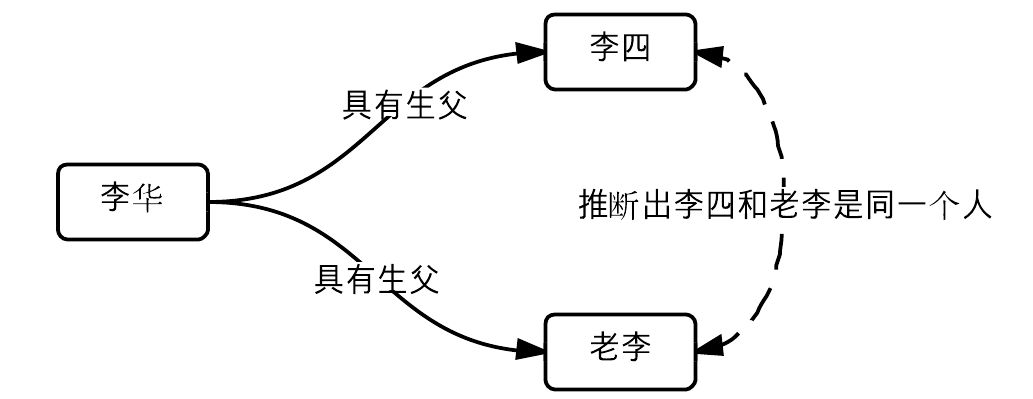
\includegraphics[width=3.5in]{fig/functionalPropertyExample.png} 
	\caption{函数属性例子}\label{fig:函数属性例子} 
	\end{figure} 
	
		\subsubsection{反函数属性}
	所谓反函数属性(Inverse Functional Properties),是指其反属性是函数的。举例说明,如图\ref{fig:反函数属性例子},如果有这样两条陈述:李四是李华的生父,老李是李华的生父,“是其生父”具有反函数属性,那么就可以推断出,李四和老李是同一个人。这样同样可以推断出同义个体。
	
	\begin{figure}[htbp] 
	\centering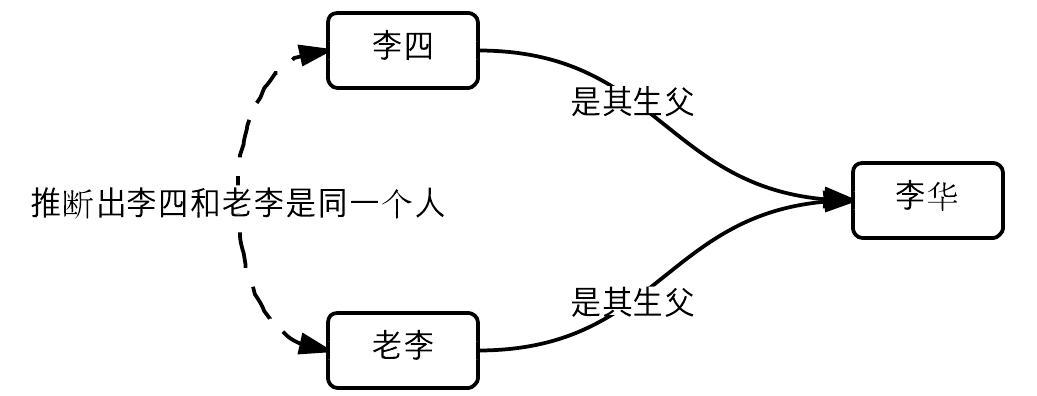
\includegraphics[width=3.5in]{fig/inverseFunctionalPropertyExample.png} 
	\caption{反函数属性例子}\label{fig:反函数属性例子} 
	\end{figure} 
	
	看起来,函数关系与反函数关系很相似,为了更准确地利用,必须加以严格的区别。对于函数关系而言,是通过主语和谓语判断出不同的宾语指的是同一个体;而对于反函数关系而言,则是通过谓语和宾语判断出不同的主语指的是同一个体。
		
		\subsubsection{传递性}
	故名思义,所谓传递性(Transitive Properties)是指,如果个体A和个体B之间存在某种关系,B和C之间也存在这种关系,那么能推理出A和C之间也存在这种关系。举个例子,如图\ref{fig:传递性属性例子}。现在有两条陈述,李华有祖先老李,老李有祖先李爷爷,有祖先被定义了传递性属性,据此,就可以推理出李华具有祖先李爷爷。在前文的概念树建模阶段,类与类的继承关系(包括子类和超类)就利用了传递性。通过传递性的扩展,子类就被推广成了后代类,超类就被推广成为祖先类,大大拓展了一个概念的扩展范围。
		
	\begin{figure}[htbp] 
	\centering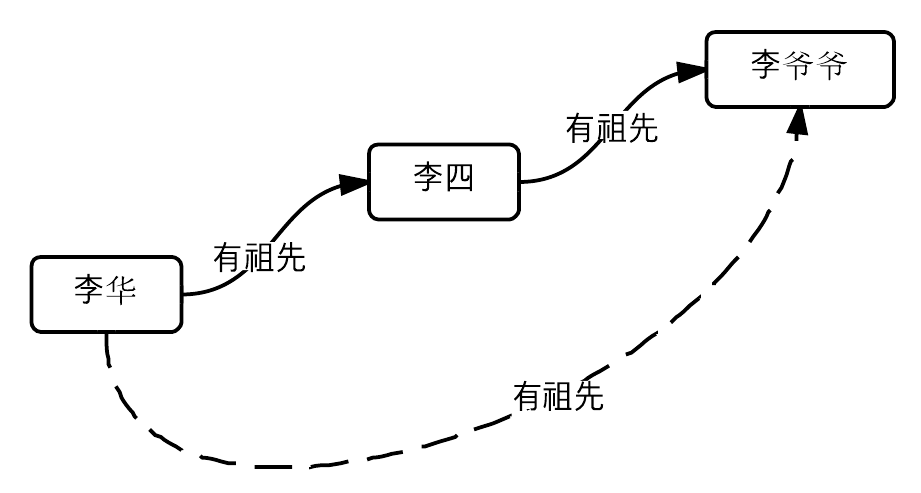
\includegraphics[width=3.5in]{fig/transitivePropertyExample.png} 
	\caption{传递性属性例子}\label{fig:传递性属性例子} 
	\end{figure}	
	
		\subsubsection{对称性}
	如果一个关系具有对称性(Symmetric Properties),也就意味着个体A到个体B具有这种关系,那么个体B到个体A也具有这种关系。如图\ref{fig:对称性属性例子},如果李华有兄弟李阳,那么根据有兄弟的对称性属性,就可以推断出李阳有兄弟李华。通过对称性,可以将单向的关系扩展成为双向的,在关系建模阶段就得到了简化。
	\begin{figure}[htbp] 
	\centering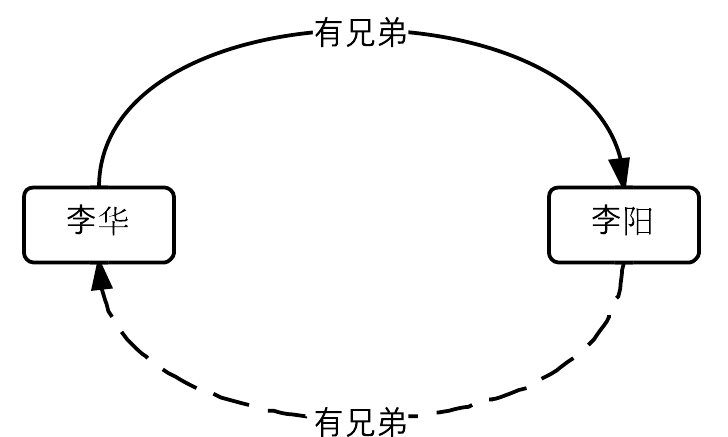
\includegraphics[width=3in]{fig/SymmetricPropertyExample.png} 
	\caption{对称性属性例子}\label{fig:对称性属性例子} 
	\end{figure}	
	
		\subsubsection{其他属性}
	反对称性(Asymmetric Properties)与对称性相反,反对称性是指,如果个体A到个体B存在关系P,那么个体B到个体A就不能具有关系P。比如,如果有一个陈述,李四有孩子李华,有孩子具有反对称属性,那么就不能存在“李华有孩子李四”这样的陈述。这种属性设置是为了检验本体的逻辑正确性,在本系统中暂时不用。
	
	自反性(Reflexive Properties)指一个关系的主语宾语是同一个体;反自反性(Irreflexive Properties)指一个关系的主语宾语不能是同一个体。这两种关系在系统中都没有运用,就不再赘述。
	
	\vspace{6pt}
	以上介绍了本体关系所具有的几种常用的属性,它们将会作为本体推理的基础。
	
	\subsection{本体推理}
	以OWL语言描述本体的一个重要好处就是可以采用推理机(Reansoner),通过推理机,可以完成三方面的功能。第一,拓展类的层次结构关系,把子类推广到后代类,把超类推广到祖先类,这样一来,可以很容易的回溯出一个概念在分类学上的线索,对于语言扩展而言,这是相当重要的,比如在检索直齿圆柱齿轮的特性的同时,系统会找到其超类——齿轮,然后找到齿轮的特性,同样,齿轮作为构件的子类,构件的性质也能被找出来,这是一个从具体的特性到抽象的共性的拔高过程,以此获取更为丰富的信息,需要注意的是,此处的推理是在类的层次进行的;第二,检验本体的一致性,也就是检验了本体各种关系的逻辑会不会出现矛盾,以此来判断本体的合理性,通过分析出现矛盾的情况,能够不断完善本体,提高本体的鲁棒性;第三,通过推理机,判断某个个体是否为某个类的个体,举个例子,定义了一个叫减速箱的类,它具有一些充要的约束条件,如具有箱体,具有数量大于2的齿轮,在检索箱体和齿轮的时候,系统就可以推理出它是一个减速箱,从而列举出减速箱的相关信息。
	
	Prot{\'e}g{\'e}提供了FaCT++等推理机,可以在建模阶段发挥检验的作用,一方面检验本体的逻辑一致性,另一方面检验推理出的关系是否如我们所预期。但是这种Prot{\'e}g{\'e}推理出来的信息并不会保存在OWL文件中,所以在之后系统可用的本体的推理功能是通过Jena实现的。Jena将会在后文进行介绍。
	
	\subsection{本体的读取}
		\subsubsection{本体的描述方式}
	前文提到了用OWL来描述本体,但是对于这样一种本体描述语言,仍有不同的变体,来实现对本体不同层次的描述。下面就进行简要介绍:
	\begin{itemize}
		\item
	RDFS(Resource Description Framework Schema,资源描述框架):也可写作RDF(S),RDF-S,RDF/S或RDF Schema。它用XML(eXtensive Markup Language,可扩展标记语言)来描述类和属性的集合,可以描述本体的的基本元素。
	
	对于图\ref{fig:生物分类}所示,这个本体就具有五个类,并且动物是生物的子类等等。在这种关系下,就可以说每个动物都是生物。所以这种类的层次关系可以理解成数学上的子集,即:$ \{动物\} \subset \{生物\} $。
	
	用RDF形式来描述这种关系,可以表示为:
	\lstset{language=XML,frame=lines}
	\begin{lstlisting}
	<owl:Class rdf:about="生物"/></rdf:RDF>
	<owl:Class rdf:about="动物">
		<rdfs:subClassOf rdf:resource="生物"/>
	</owl:Class>
	\end{lstlisting}
	第一部分建立了一种名为“生物”的类,第二部分建立了一种为“动物”的类,并且定义了它是“生物”类的子类。
		\item
	OWL:OWL是RDFS的一种扩展,RDF能完成的它都能完成,同时它又多了一些扩展功能。比如对立关系,可以通过把两个类设置成对立关系(Disjointed),这样就保证了,不能有一个个体同时是两个类的实体。再比如,通过OWL可以设置上文所述的传递性、对称性等关系特性,这就大大的拓展了本体的表达的推理的基础,而RDFS只能建立类的层次结构。
	
	OWL语言具有三种子语言:OWL Lite,OWL DL和OWL Full。OWL DL和OWL Lite让层次关系更容易被追溯;OWL DL可以使用描述逻辑推理机(Description Logic Reasoner),使其具有更强大的查询功能;OWL Lite则更利于使用一些简单的推理算法。

	\end{itemize}
	
	总体来说,本体有着不同的描述语言,从最强大的OWL Full到最精简的RDFS,建立时要根据需要进行合理选择。
		
		\subsubsection{Jena的应用}
	上文提到,采用Prot{\'e}g{\'e}进行了本体建模,建立了以OWL语言描述的本体。下面需要对本体进行读取和推理等操作,Jena是Apache软件基金会资助的项目,它是一种Java框架的语义网构建应用,它提供了方便易用的读取、加工、编写RDF数据的API以及操控RDFS和OWL本体的API。系统采用Jena工具包,实现了本体与搜索引擎的交互,下面对一些关键的API进行简要介绍。

	本体导入:
	通过ModelFactory类可以以如下代码建立本体模型:
	
	\lstset{language=Java,frame=lines}
	\begin{lstlisting}
OntModel m = ModelFactory.createOntologyModel();
	\end{lstlisting}
	
	在无参数的情况下,可以获得一个以OWL Full语言描述的、常驻内存的、具以推理子类、超类功能的推理机的模型。当然,在某些情况下,这种设置都太强了;而在某些情况下,这样的功能又显得局促。在Jena中,可以用OntModelSpec对象来设置createOntologyModel方法的参数,来对建立的模型进行配置。根据系统的实际需要,采用OWL\_DL\_MEM\_RDFS\_INF 参数进行模型建立与配置,这样就可以获得以OWL DL语言描述的、常驻内存的、具有RDF层衍生规则的规则推理机的本体模型。
	
	对于每一个本体模型,还需要有一个对应的文档管理器来协助完成操作、加工的工作,OntDocumentManager就起到了这种沟通本体文件与本体模型的功能。通过OntDocumentManager类的addAltEntry方法,可以建立系统公共本体文URI和本地本体文档URI的映射,再使用OntModel类的read方法,就可以按设定的格式进行本体读取。
	
	\begin{lstlisting}
OntDocumentManager dm = model.getDocumentManager();
dm.addAltEntry(docURI,locationURI);
model.read(docURI,"RDF/XML");
	\end{lstlisting}	
	
	经过试验验证,只有“RDf/XML”能够与Prot{\'e}g{\'e}建立的以“RDf/XML”格式存储的本体进行无缝的衔接。以上完成了对本体的读操作,通过设置推理机,很容易地获得了扩展之后的本体。下面就要根据搜索的需求,先找到一个关键词在本体中的位置,进而枚举已经定义的关系,找到与之相关的概念。如果把关键词当作根结点,把各种关系当作第二级结点,把相关的概念当作第三级结点,那么这就构成了一棵深度为3的树,我们要做的就是对这棵树进行深度优先的遍历,列举出所有“主-谓-宾”三元组关系(Triple)。
	
	这种列举操作类似对于数据库的查询操作,在数据库有查询语言SQL,在本体中也存在相类似的查询语言——SPARQL。
	
	首先要对一些概念进行解释。之前反复提到了将本体看成一张图$ G=(C,R) $,RDF图就是表示这种图的一种表示方式。根据W3C组织的定义\cite{w3c},RDF图(RDF Graph)是RDF三元组(RDF Triple)的集合。RDF三元组包含三个部分,主语(Subject),谓语(Predict),宾语(Object)。
	$$主语\ \xlongrightarrow{谓语} 宾语$$
	
	需要注意区分的是,RDF是一种应用与应用间交换信息的框架,即资源描述框架;RDFS是一种基于XML的本体描述语言;而RDF图是一种图,是三元组的集合。SPARQL的搜索对象是RDF图,它具有与SQL相类似的语法。比如要检索齿轮(Gear)的子类,可以用下列的SPARQL。
	\lstset{language=SQL,frame=lines}
	\begin{lstlisting}
SELECT ?x
WHERE {?x <SubClassOf> "Gear"}
	\end{lstlisting}	
	但是当主语、宾语处在多层嵌套,这种语法会变得异常复杂,而且需要对RDF图的细节有较深的了解,对于一般用户难以灵活自如地运用。但是Jena为我们提供了丰富易用的类可以胜任这个工作。

	
	操作本体:		
	在Jena中,每个概念作为一个OntClass类的对象进行存储。用Model类的getOntClass方法,以类节点的URI为参数,这样就可以确定关键词在本体中的位置,完成主语的确定。
	
	下面就要枚举出所有的关系,找到所有谓语。谓语可以通过两种分类方法,分成六类,如表\ref{tb:谓语分类}

\begin{table}[htbp]
\centering
\caption{\label{tb:谓语分类}谓语的分类}
\begin{tabular}{c|c|c|c}
\Xhline{1.5pt}
 & 超类 & 等价类 & 子类\\
\hline
 普通类 & 普通超类 & 普通等价类 & 普通子类\\
\hline
 约束性类  & 约束性超类 & 约束性等价类 & 约束性子类\\
\Xhline{1.5pt}
\end{tabular}
\end{table}

	超类、等价类、子类这种分类方法是基于概念的层次结构的,而普通类和限性性类则是基于建模不同阶段的。对于第一种分类方法,它们的区别仅在于概念层次结构的细微差异,处理方法是类似。下面主要讨论普通类和约束性类的区别及不同的处理方法。
	
	普通类谓语是在概念层次结构阶段的建模就具有的,这种谓语关系已经被蕴含在了概念树结构中,其OWL语言表述如下
	
	\lstset{language=XML,frame=lines}
	\begin{lstlisting}
<Class rdf:about="4-Bar_Linkage_mechanism">
 <rdfs:subClassOf rdf:resource="Linkage_Mechanism"/>
</Class>
	\end{lstlisting}
	
	这样就定义了连杆机构和四连杆机构的继承关系,可以观察到谓语“subClassOf"的宾语是一个普通的概念。
	
	另一种情况是约束性谓语,约束性谓语则相对复杂,如上文建立关系部分所提到的,我们采用了对象属性来描述概念与概念之间的关系,但是根据官方说明,对象属性是用来描述个体关系的,所以,必须要采用一定的转化机制。在本体中,恰提供了这样的机制——约束(Restriction)。将上一段代码所表示的关系进行扩展,在“四连杆机械是连杆机构”的描述之后,又加了一条“四连杆机构具有构件连杆”,“具有构件”就是自己定义的对象属性,用OWL的表示方法如下:
	
	\begin{lstlisting}
<Class rdf:about="4-Bar_Linkage_mechanism">
 <rdfs:subClassOf rdf:resource="Linkage_Mechanism"/>
 <rdfs:subClassOf>
  <Restriction>
   <onProperty rdf:resource="has_Some_Links"/>
   <onClass rdf:resource="Linkage"/>
   <qualifiedCardinality rdf:datatype="&xsd;nonNegativeInteger">
    3
   </qualifiedCardinality>
  </Restriction>
 </rdfs:subClassOf>
</Class>
	\end{lstlisting}
	
	容易观察到,系统处理以对象属性作为概念间的关系的方法是:把真实的谓语和宾语封装成为一个约束,这个约束再作为“subClassOf”的宾语。约束中主要包括三种元素:真实的谓语(即对象属性),真实的宾语(即相关概念),约束类型。
	
	知道了这种机制,在迭代器获得关键词概念的下一个超类(或等价类,或子类)的时候,先判断出它是普通类谓语还是约束性谓语,再分别作出对应的处理,就可以实现上述的“主-谓-宾”三元组关系的列举,把这些关系封装成一个Triple类的对象,以备之后使用。Triple对象在后文中介绍。至此,基本完成了与本体相关的操作:建模,读取,操作,使用。	
	
	\subsection{Prot{\'e}g{\'e}介绍}	
	前文反复提到了我们所使用的本体建模软件Prot{\'e}g{\'e},Prot{\'e}g{\'e}是由斯坦佛大学与曼彻斯特大型合作开发的一款免费的开源的本体编辑器和基本知识框架。它基于Java框架,具有极强的扩展性,通过丰富的插件,可以实现快速的原型开发与应用开发。Prot{\'e}g{\'e}具有相当友好的图形界面,灵活直观地展现本体模型的体系结构与概念间错综复杂的关系。Prot{\'e}g{\'e}也提供了RDF/XML,OWL/XML,Turtle等丰富的存储格式,由于Prot{\'e}g{\'e}的开发本身就大量地使用了Jena包,它们的深度集成为本系统从本体建模到本体操作提供了无缝衔接提供了支持。
	
\newpage
\section{扩展性语义搜索算法}
\setcounter{figure}{0}
\setcounter{table}{0}
\setcounter{equation}{0}
	
	在前文所述的工作中,我们完成了本体的构建,并且获得了读取操作本体的方法,本部分就要以此为基础,实现扩展性语义搜索算法。首先介绍扩展性语义搜索算法的原理,然后介绍一些关于搜索的基本方法概念,阐述系统是如何运用相关工具包实现搜索,提出搜索结果的排序依据,最后提出对搜索引擎评价的两种指标。
	\subsection{原理}
	
	前文提到,普通的基于关键词的搜索是通过简单的编码匹配,这样的方式甚至不能解决最基本的同义词问题,就更别说实现语义的扩展了。对于一个理想的人工智能的系统来说,我们希望它能理解我们的意思,但要表达我们的意思,还是需要以语言作为载体。这种载体不能像SPARQL查询语言那样艰深,尽管它有强大的查询能力,但还是让大多数用户望而生畏。扩展性语义搜索算法的核心理念就在于,让用户就像在使用普通的关键词搜索那样操作,却获得远远超越普通关键词搜索的性能。这种思想的实现得益于以本体来描述知识的方式,通过简单的同义词关系,我们就获得了同义词搜索的功能,通过本体中定义的其他丰富概念之间存在的关系,我们就获得了语义扩展的功能。
	
	实现思路是,用户输入关键词,在本体中找到该关键词并获取与之有关系的概念词,把关键词与概念词一并作为搜索关键词进行加权搜索,获得搜索结果。如图\ref{fig:搜索算法流程}。
	
	\subsection{实现}
		\subsubsection{Lucene}
	Lucene同样是Apache基金会支持的项目,是一个开源的全文检索引擎工具包,是一个包含了查询引擎、索引引擎及部分分析引擎的完整架构。Lucene 定义了一种以 8 位字节为基础的索引文件格式 ,可以轻松地实现跨平台下共享索引文件,同时由于众多优秀的程序员对 Lucene 做出卓越贡献,使得 Lucene 能够提供极高的搜索效率,包括苹果公司等众多商业场合,都用在使用 Lucene 进行搜索。Lucene的后台极其复杂,运用了先进的信息检索技术,但是它提供了丰富易用的API屏蔽了后台的复杂机制,普通编程者可以很容易地在目标系统中进行全文检索。
	
	Lucene很容易被误解成一个完整的搜索程序,但它其实只是一个搜索程序的两个核心模块,即索引和搜索。下面就简要介绍一个搜索程序的架构。如图\ref{fig:搜索程序架构}。
	
	\begin{figure}[htbp] 
	\centering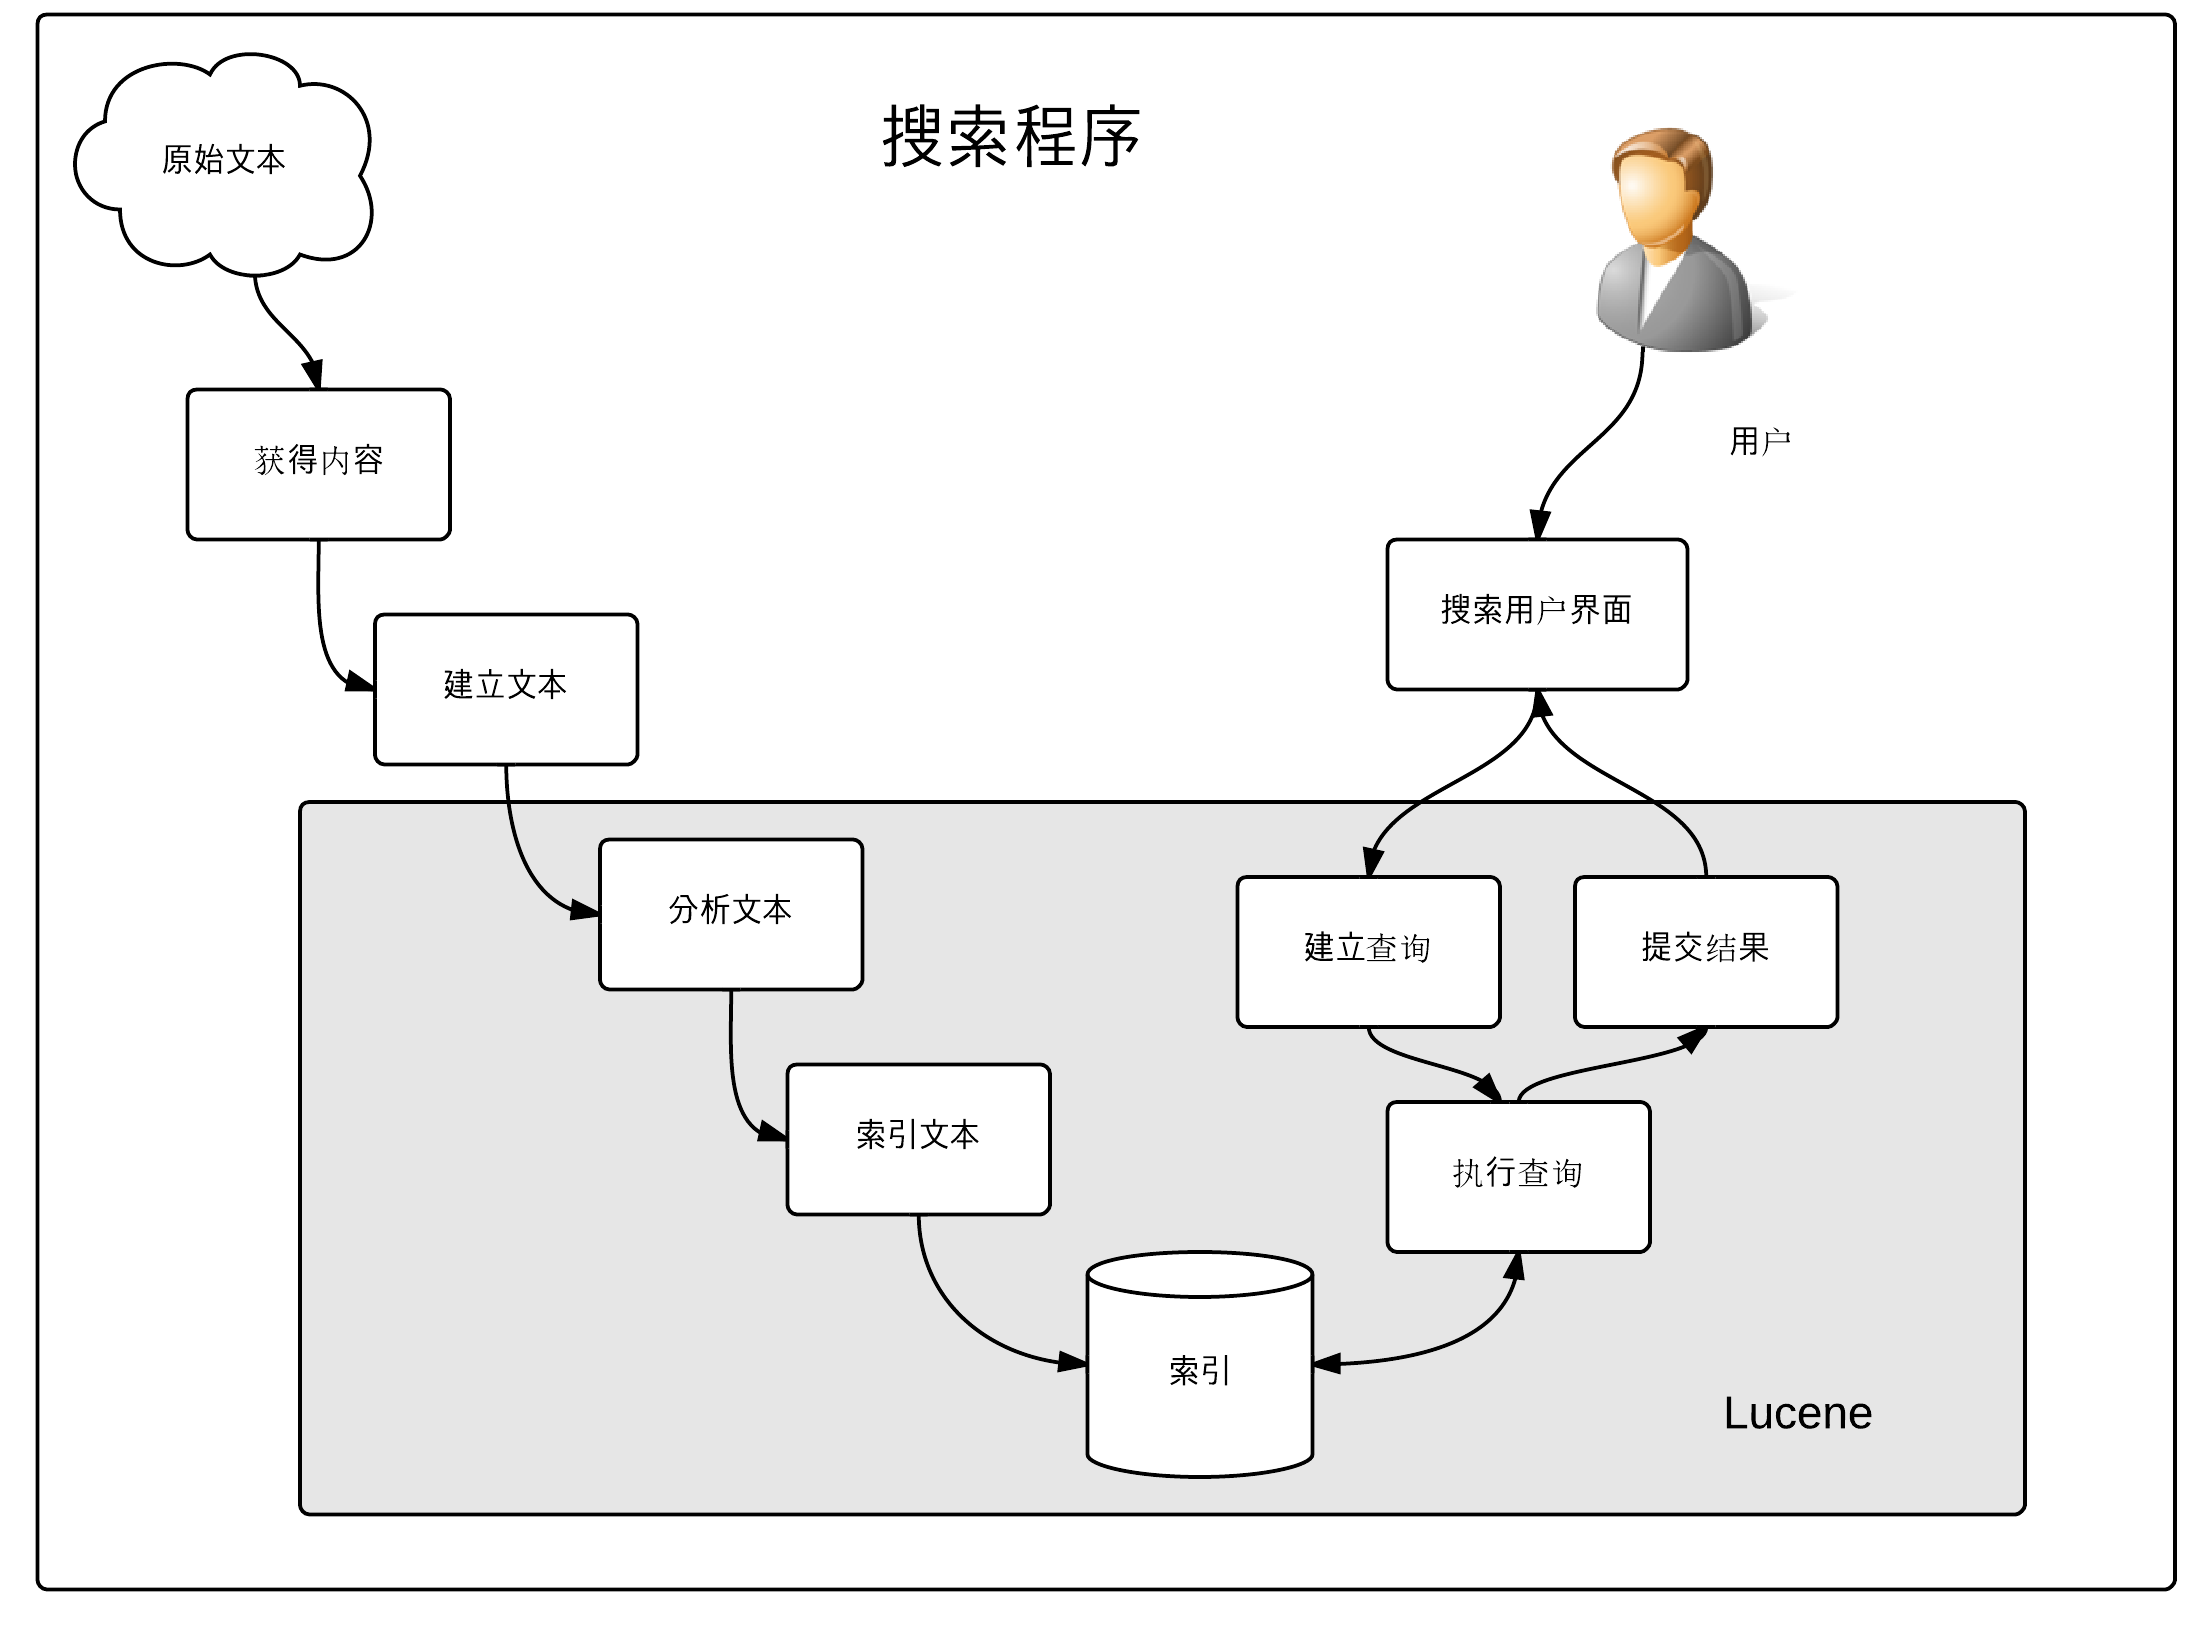
\includegraphics[width=5in]{fig/SearchEngineFrame.png} 
	\caption{搜索程序架构}\label{fig:搜索程序架构} 
	\end{figure} 
	
	可以看到,对于一个搜索程序,首先它需要从原始文本中获取内容,建立文档并分析它们,生成一个索引文档并放在索引中,当用户有搜索请求时,他会在用户界面上中输入他的查询要求,然后系统建立并执行一个查询(Query),在索引中获得该查询的相关信息,然后将搜索结果进行的一定的加工,再在用户界面上呈现出来。对于Lucene,它完成的是整个架构中的深色部分,当然也是至关重要的部分。下面就对这两个部分进行介绍。	
	
		\subsubsection{索引}
	搜索的任务就是要找到具有特定关键字的文件,一种朴素的方法是顺序扫描每个文件,检验文件中是否含有要这个关键字,在不记任何成本的情况下,这样做应该是可以达到目的的。但是试想,如果搜索的对象是具有庞大数据量的数据集,或是庞大的单个文件,这种搜索方法的效率势必是极低的。所以在进行搜索操作之前,需要把文档转换成一种能够快速搜索的格式,这种转换过程就是所谓索引操作(indexing),其输出结果就是索引(index)。下面以倒排索引为例,解释为什么通过索引可以提高搜索效率。
	
	倒排索引(Inverted Index),亦称反向索引、置入档案或反向档案,是众多索引方式中较为常用的一种,它建立了一个词在单个或多个文档的映射,这样就可以根据词快速确定存在该词的文档列表。比如对于以下三个文本:
	
	$T_0 = "What\ is\ lucene?"$
	
	$T_1 = "Lucene\ is\ for\ search."$
	
	$T_2 = "What\ is\ search?"$
	
	经过索引操作之后,就可以获得如下索引:
	\begin{lstlisting}
	"what":   {1,3}
	"is":     {1,2,3}
	"lucene": {1,2}
	"for":    {2}
	"search": {2,3}
	\end{lstlisting}
	
	通过这样的机制,就建立了简单的索引文件。当然,根据需要,还可以把词在文档中的位置信息存储在索引中。实际的索引比这个要复杂很多,但索引的技术细节并不我们的研究对象,此不赘述。
	
	下面介绍系统是如何使用Lucene建立索引,从而得到功能集中的索引器的。
	在Lucene中,要执行一个简单的索引操作需要用到以下几个类:
	
	\begin{itemize}
		\item IndexWriter(写索引)
		\item Directory(目录)
		\item Analyzer(分析器)
		\item Document(文档)
		\item Field(域)
	\end{itemize}
	
	IndexWriter是索引操作的核心类,它负责完成新建或打开索引,并且执行添加、删除及更新等操作;Directory类则为IndexWriter存储的索引开辟空间,同时通过FSDictory.open方法,可以建立待索引文件在文件系统中的目录与索引文件之间的对应关系;在上述的简单的索引的例子中,是人工的采用了以空格来区分单词的方法,但在实际使用中,这种方法可能是不完备的,这就需要有一种机制,来对文本进行解析处理,Analyzer类就是完成这件事情的,它将文本进行合理的划分,提取词汇单元,筛选掉无用信息;文档是域的集合,Document类就实现了文档的功能;域则保存了不同种类的文本信息,比如对于一个音乐文件,其文件名、作者、专辑名等元数据都会被存在不同的Field类中,进而被包成一个Document类。通过这些一系列的步骤,就可以完成索引操作。实现索引操作关键代码如下:
	
	\lstset{language=Java,frame=lines}
	\begin{lstlisting}
//声名一个写索引器	
IndexWriter writer = null;

//打开实际文件系统中的文件目录
Directory dir = FSDirectory.open(new File(indexPath));

//配置写索引器,设置索引存储空间、分析器、创建或重写及最大文件数
writer = new IndexWriter(dir, 
			new StandardAnalyzer(Version.LUCENE_30), 
			true,
			IndexWriter.MaxFieldLength.UNLIMITED);

//声明一个Document类
Document doc = new Document();

//建立内容(CONTENTS)域,配置域名、待加工内容、域存储选项及域的项向量选项
Field contents = new Field(CONTENTS, 
				stuff.getContents(), 
				Field.Store.YES,
				Field.Index.NOT_ANALYZED);
					 
//以类似的方法,建立文件名域,文件ID域

//将之前建立的各域写进文档
doc.add(contents);
	\end{lstlisting}
	
	在实际建立索引过程中,每个域并不是被等同创建的。比如,如果要搜索关键词“齿轮”,其他条件都相同的情况下,一个文件的文件名包含一次“齿轮”,另一个文件的文本内容包含一次“齿轮”,显然前者更有可能是用户要找的文本,这就要求对不同的域采用恰当的权值进行加权操作。加权操作可以在索引期间完成,也可以在搜索期间完成。由于后者虽然动态性较加,可以在搜索期间进行灵活的权值确定,但这会消耗掉一定的CPU效率。所以,系统选择在索引期间进行加权,在一些特殊情况,也可以在搜索期间把索引期间所加的权值补偿回来,这样既保证了效率,又提供了足够的灵活性。在Lucene中,可以通过setBoost方法对文档和域进行加权操作。在此,将文件名域(filename)权值设置得略高于内容域(contents)的权值,以突出文件名在搜索中的重要性。在一定的评价指标下,可以通过改变权值配置,进行搜索的优化。
	为了方便信息的传递,通过Lucene获得的搜索结果将会是一个文件ID号,通过这个ID号,可以在数据库中找到对应的文档,还可以获得其他未在索引中建立,但是存储在数据库中的信息。
	
		\subsubsection{搜索}
	建立了索引,提供了一种快速检索的机制,但是索引终究是处于后台的,要让其强大的功能得以表现,还需要有搜索作为一个窗口。下面就要针对索引,建立相应的搜索程序,简要介绍搜索会用到的几个基础类。
	
	\begin{itemize}
		\item IndexSearcher(索引搜索)
		\item Query(查询)
		\item QueryParser(查询解析器)
		\item TopDocs(顶部文档)
		\item ScoreDoc(评分文档)
	\end{itemize}
	
	IndexSearcher类是搜索的门户,由它完成通过索引进行的搜索操作。在实际运用中,它与其他相关类的关系如图\ref{fig:IndexSeacher类与相关类的关系}。
	
	\begin{figure}[htbp] 
	\centering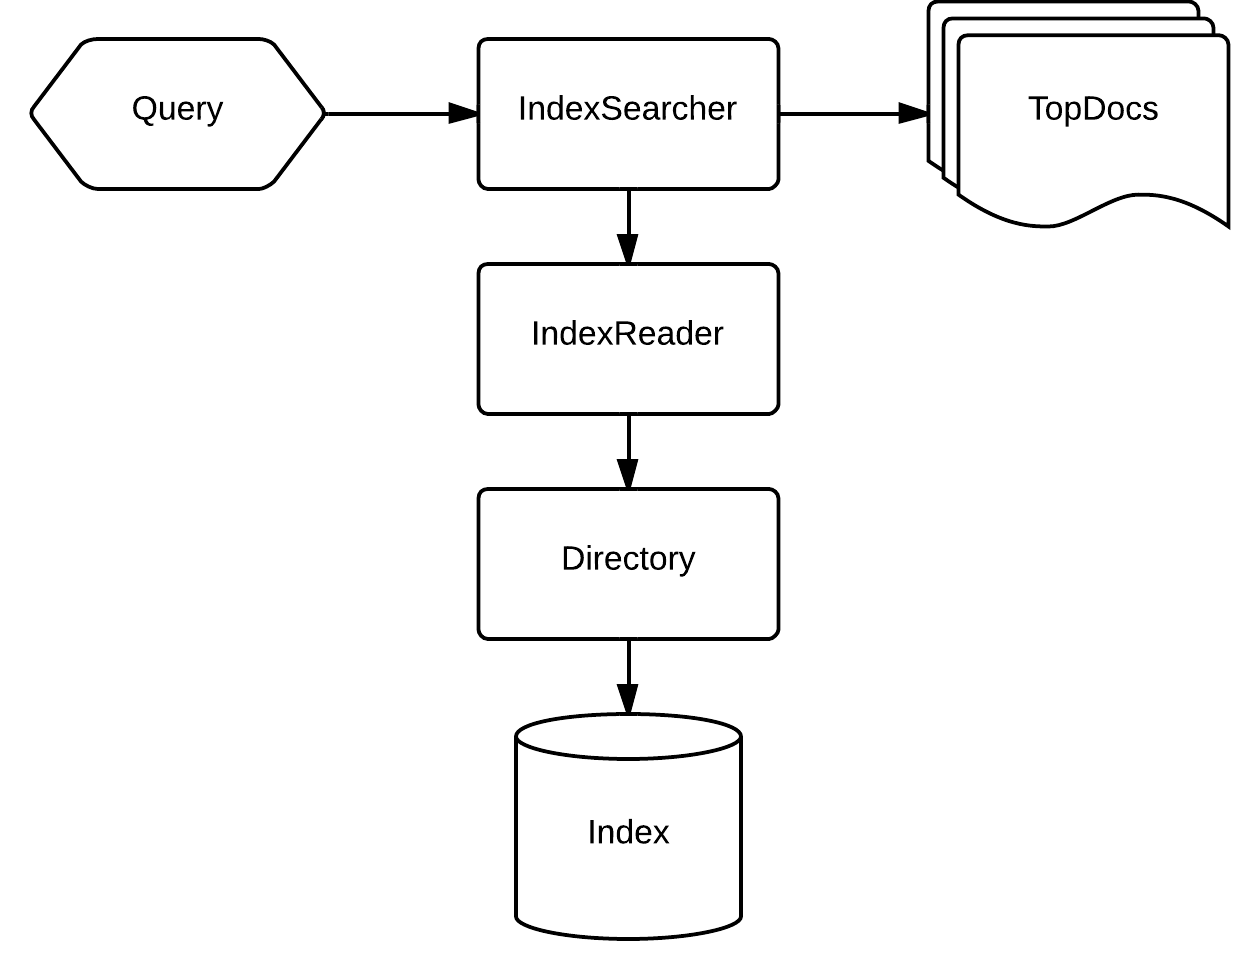
\includegraphics[width=4in]{fig/IndexSearcher.png} 
	\caption{IndexSeacher类与相关类的关系}\label{fig:IndexSeacher类与相关类的关系} 
	\end{figure} 
	
	在初始化阶段,建立Directory对象用以开辟读取索引文件Index文件的空间,用一个IndexReader类对象来读取索引文件,IndexReader需要较大的系统开销,所以在搜索过程中,最好只建立一个IndexReader实例。下面就是搜索阶段,当IndexSearcher对象接收了一个Query类的对象,它就会用search方法调用通过相关类调用索引文件,获得搜索结果,进行评分等工作,最后输出一个TopDocs类的对象作为搜索结果。	
	\vspace{6pt}
	
	Query是一种查询请求的封装,IndexSearcher类接收Query对象作为查询的参数。针对不同的搜索要求,Query有不同的子类来实现相应的功能,如TermQuery、 NumericRangeQuery、 TermRangeQuery、 PhraseQuery、 PrefixQuery、 FuzzyQuery、 WildcardQuery、 BooleanQuery以及MatchAllDocsQuery等,它们可以完成通过项搜索、通过指定数字范围搜索、通过指定项范围搜索等功能、短语搜索、前缀搜索、模糊搜索、通配符搜索、布尔搜索以及匹配所有文档搜索。这些子类可以被直接实例化,可以通过QueryParser相应的子类来实例化,我们采用后一种方法。
	\vspace{6pt}
	
	QueryParser类能把用户输入的查询表达式进行解析,把查询拆分成若干个项(term)(项是最小的索引片段,它包含了一个域名和一个文本值),进而封装成一个Query类的对象。
	
	举个较为复杂的查询表达式的例子:“Cam\^{}4 (Link)\^{}1 (Vedge AND Cam)\^{}1 (Disc AND Cam)\^{}1 (Cylindrical AND Cam)\^{}1”,所谓解析,就是要把这种表达式转换成若干个项,再封装成对应的Query实例。流程及类的关系如图\ref{fig:QueryParser}。
	
	\begin{figure}[htbp] 
	\centering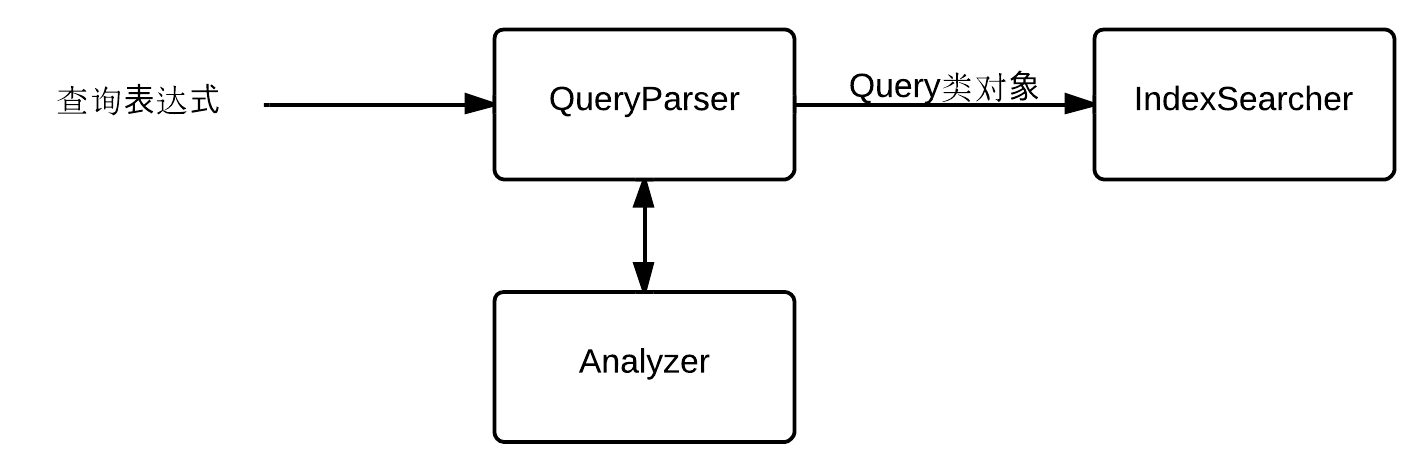
\includegraphics[width=4in]{fig/QueryParser.png} 
	\caption{QueryParser工作流程及与相关类关系}\label{fig:QueryParser} 
	\end{figure} 
	
	当QueryParser接收到一个查询表达式(这个表达式可能是由用户输入,也可能是由系统生成),它就会利用分析器(Analyzer)进行分词操作把查询语句分割成多个项,进行大小写转换等处理,再封装成一个Query类的对象,传送给IndexSearcher类。
	
	事实上,一个详细的查询表达式,能够更精确地描述查询意图。表\ref{tb:查询表达式范例}就列举了一些查询表达式的语法结构。
	
\begin{table}[htbp]
\centering
\caption{\label{tb:查询表达式范例}查询表达式范例}
\begin{tabular}{c|c}
\Xhline{1.5pt}
 查询表达式 & 匹配文档\\
\hline
 Gear  & 默认域包含Gear项的文档 \\
\hline
 Gear Mechanism  & 默认域包含Gear和Mechanism项中一个或两个的文档\\
\hline
 Gear  OR Mechanism  & 默认域包含Gear和Mechanism项中一个或两个的文档\\
\hline
 +Gear +Mechanism  & 默认域同时包含Gear和Mechanism项的文档\\
\hline
 Gear  AND Mechanism  & 默认域同时包含Gear和Mechanism项的文档\\
\Xhline{1.5pt}
\end{tabular}
\end{table}
	通过这些逻辑表达式可以更精确地限制搜索的范围。
	
	如前文所提到的,针对不同的搜索要求,Lucene提供了不同的查询子类,这些子类可以由不同的解析器来进行实例化。在我们的搜索算法中,一个很重要的功能是加权,Lucene提供了相对应的功能。在一个项后面加一个“\^{}”符号再跟一个浮点数,就会对该项查询处理进加权因子的设置 。比如,查询表达式为“Cam\^{}4 (Link)\^{}1”,那么Cam的TermQuery的加权系数设为4,而将Link的TermQuery设置为1。加权系数如何影响结果的排序将会在后文中有阐述。
	
	之前在索引的部分提到,在索引操作的过程中,建立了文件名域和内容域两个域,用户会更倾向于同时对两个域进行搜索,而不是只针对其中一个。要实现这样的多域搜索功能,可以用建立全包含域的索引的方法,也就是将把所有域的内容全拼接在一块儿,形成一个包含所有内容的域,再对这个域进行索引,这种方法虽然在搜索效率上不错,但是显然,字符串的简单连接使得它不能进行域的加权操作。这里系统采用了用MultiFieldQueryParser的方法。
	
	MultiFieldQueryParser是QueryParser的子类,它能在后台把一个QueryParser实例化,分别针对每个域解析查询表达式,再用BooleanQuery将它们连接在一块儿。
	\lstset{language=Java,frame=lines}
	\begin{lstlisting}
//多域查询解析器
QueryParser multiFieldParser = new MultiFieldQueryParser(Version.LUCENE_30, 
		new String[] {"filename", "contents"},
		new StandardAnalyzer(Version.LUCENE_30));
	\end{lstlisting}
	
	这样,就可以同时针对文件名域和内容域进行搜索,并且能够利用之前对它们进行的域的加权操作。
	
	\vspace{6pt}
	
	TopDocs类是一个简单的指针窗口,其对象保存了IndexSearcher获得的得分较高的搜索结果。它提供了两个属性,totalHits用以表示匹配搜索条件的文档数量,scoreDocs是一个scoreDoc类的数组,通过遍历scoreDocs属性,可以逐个获得搜索结果;TopDocs还提供了getMaxScore方法,用来返回最大评分。尽管评分对于普通用户是隐性的,但是在系统调试阶段,这样的评分会作为评估系统搜索性能的重要依据。
	\vspace{6pt}
	
	ScoreDoc类则提供了对搜索结果访问的丰富接口
	\vspace{6pt}。
	
	采用这些类,就可以实现一个搜索,它即保证了基本的搜索功能,也能完成我们所设计的搜索算法。
	
		\subsubsection{排序依据}
	
	如式\ref{eq:1}所描述的,搜索归根结底是一种文档与评分的映射,之前反复提到了搜索结果排序,对域或项进行加权操作等,那么文档是如何评分的,对域或项的加权操作又是如何影响评分的呢?Lucene提供了一套完整成熟优秀的评分机制,其核心是相似度评分公式,计算方式是查询语句(q)的各项(t)与文档(d)的匹配程度,它深刻地描述了查询语句与对应匹配文档的相似度:
	\begin{equation}\label{eq:luceneScore}
	\begin{aligned}
SC = \sum_{t\ in\ d}&(tf(t\ in\ d)\times idf(t)^2 \times boost(t.field\ in\ d) \times lengthNorm(t.field\ in\ d)) \\
   				    & \times coord(q,d) \times queryNorm(q)
    \end{aligned}
	\end{equation}
	
	下面就逐个来解释各个评分因子:
	\begin{itemize}
		\item
	$ tf(t\ in\ d) $:tf(term frequency)项频率因子。
	\begin{equation}\label{eq:tf}
	tf(t\ in\ d)=\frac{n_{t\ in\ d}}{\sum_{i \in d}{n_{i\ in\ d}}}
	\end{equation}
	$ {n_{i\ in\ d}} $指一个项(i)在文档(d)中的出现次数 。	
	项频率因子描述了在某个文档(d)中出现查询项(t)的频率,它是对词数的归一化,以避免它偏向较长的文件。因为在较长的文件中,无论它重要与否,某个项可能出现的次数都有增多的趋势。
		\item
	$ idf(t) $:idf(inversed document frequency)逆向文件频率因子。
	\begin{equation}\label{eq:idf}
	idf(t)=log\frac{|D|}{1+|\{ j:t \in d_j\}|} 
	\end{equation}
	$ |D| $表示文档总数,$ |\{ j:t \in d_j\}| $表示包含了项(t)的文档数。分母加了1是为了避免出现项(t)未在任何文档中出现而造成分母为零的情况。
	
	逆向文件频率因子可以评价项的“唯一”性,定性地说,在包含项(t)的文档(d)越少,该因子越大,因此它具有很高的类别区分能力。
		\item
	$ boost(t.field\ in\ d) $:域或文档的权值,如前文介绍,这个权值可以是在索引期间建立的,比如本系统的域加权部分;也可以是在搜索过程中建立的,比如本系统的项加权部分。
		\item
	$ lengthNorm(t.field\ in\ d) $:域的归一化值(Normalization),它表示了域中所包含项的数量。域的归一化值在索引操作期间建立,然后保存在norm索引中。对于域的归一化值,越短的域,词汇单元越少的域将会获得越大的加权。
		\item
	$ coord(q,d) $:协调因子(Coordination factor),这是基于文档中所包含的查询的项数来确定的。协调因子对包含更多搜索项的文档进行类似AND的加权。
		\item
	$ queryNorm(q) $:查询的归一化值,即查询语句(q)中每个查询项(t)权重的平方和。
	\end{itemize}
	
	由此可见,在一串其貌不扬的具有一定顺序的搜索结果背后,隐含着复杂的统计公式。为了给编程者提供定量分析依据,Lucene提供了Explanation类。IndexSearcher类的explain()方法通过一个Query对象和文档的ID作为参数,可以获得一个Explanation类的对象,它包含了所有关于评分计算中各因子的信息。在系统后台,可以以结果评分为依据,对权值设置进行调整,进而优化搜索系统。	
	
	\subsection{评估指标}
	建立好了搜索系统,就要对系统进行相关性和搜索质量进行评估。对于一个搜索系统来说,如果用户没有得到他想要的结果,那么将算法描述得再怎么巧妙也是无济于事的。一个用户要求搜索系统做到什么呢?首先,程序返回相关的文档,其次结果摘录是精确的,然后用户能在第一眼就看到他们想要的结果,等等。文献\cite{buttcher2010information}介绍了关于评价搜索系统的指标。评估指标需要具有具备一些条件:
	\begin{itemize}
		\item
	指标要能描述一种能表达完成搜索预期目标的特征,比如之前所提到的相关性特征。
		\item
	指标要能够定量描述完成搜索预期目标的效果。
		\item
	指标所采用的度量技术要精确而经济。
		\item
	指标要能够进行误差估计。
	\end{itemize}
	在此,我们介绍两种较为简单、常用的评价指标。
		
		\subsubsection{查准率及查全率}
	查准率和查全率都是传统的有效性指标,它们都是基于两个基本假设的\cite{buttcher2010information}:
	\begin{enumerate}[1)]
		\item
	对于一个用查询来表示的用户信息需求(information need),且在一个文档集合中,那么文档集中的每个文档与这种用户的信息需求要么相关,要么不相关。
		\item
	信息需求和文档就能完全确定文档的相关性,相关性与文档集中其他文档的搜索引擎排名无关。
	\end{enumerate}
	
	查全率和查准率被用来评价搜索系统在响应某个查询时检索出来的无序的文档集合,它们可能是信息检索评价指标中最古老、最朴素的。
	
	查全率(recall)描述了搜索结果的文档集中相关文档所占的比例,根据这个定义,如果用Resu表示被检索出来的文档集合,用Rela表示相关文档集,那么查全率就可以表述为:
	\begin{equation}\label{eq:recall}
	recall = \frac{|Resu\cap Rela|}{|Rela|}
	\end{equation}
	
	容易发现,查全率在描述了相关度文档所占的比例,但它很容易就能实现1.0的查全率——只要将文档集中所有文档作为结果返回即可。这样虽然保证了相关文档都在返回文档集合中,却不能保证返回的文档集合里的文档都是相关文档。所以再引入查准率(precision)来评价,即搜索系统检索出的相关文档占检索出的全部文档的比例,表述为:
	\begin{equation}\label{eq:recall}
	precision = \frac{|Resu\cap Rela|}{|Resu|}
	\end{equation}
	
	从以上查全率、查准率的定义可以看出,它们确实能够一定程度上刻画搜索结果的优劣。但是它忽略了排序对于一个搜索系统的重要作用,用户一般会采用从上到下,从前往后的顺序进行检查,检查每一个文档都会付出一定的代价,所以能够排在前面的条目当然更应该是用户所想要的结果。在这种前提下,用户按一定顺序进行检查,那么查全率、查准率都会随着检查过程发生变化。要准备地描述这种变化,就要绘制P-R图(查准率-查全率图)。
	
	举个例子,对于一个确定文档集及信息查询实例,包含查询q的相关文献的集合R是确定了的,不失一般性,假设R由下列文档组成:
	$$ R = \{d_{2},d_{5},d_{23},d_{31},d_{57},d_{89},d_{97},d_{111},d_{137},d_{229}) $$
	
	现在由一个搜索系统以查询q进行搜索,返回了搜索结果:
\begin{multicols}{4}
\begin{enumerate}
\item $d_{137} \surd$
\item $d_{23} \surd$ 
\item $d_{4}$
\item $d_{5} \surd$ 
\item $d_{112}$
\item $d_{92}$
\item $d_{57} \surd$
\item $d_{23} \surd$
\item $d_{67}$
\item $d_{55}$
\item $d_{101}$
\item $d_{34}$
\end{enumerate}
\end{multicols}

	打勾的结果d是与查询q相关的文档,即$d_i \in R$。下面按照搜索的结果开始逐个检查,分别计算其查全率和查准率,步骤如下:
\begin{enumerate}[a)]
\item
搜索结果中的第一篇文档$d_{137}$是相关的,得出查准率是100\%,总共有十篇相关文档,现在找到一篇,查全率是10\%;
\item
第二篇文档$d_{23}$是相关的,进行类似的计算,得到查准率是100\%,查全率是20\%;
\item
到了第四篇文档$d_{5}$,查准率是75\%,查全率是30\%;
\end{enumerate}

	重复这个操作,就可以达到一组查准率-查全率的点,从而得到P-R图。通过以上数据,绘制出相应的P-R图,如图\ref{fig:p-rFigure}。
	\begin{figure}[htbp] 
	\centering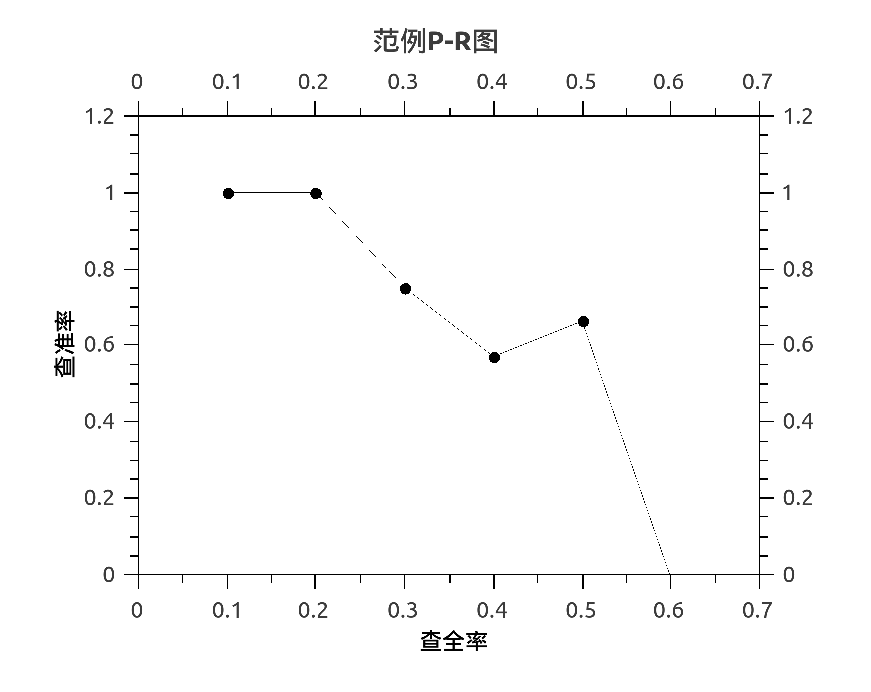
\includegraphics[width=4in]{fig/prFigureExample.eps} 
	\caption{范例P-R图}\label{fig:p-rFigure} 
	\end{figure} 
	
	在上面的例子中,是针对一个查询请求的,但是在实际性能测试中,应该通过不同的查询来评价搜索算法。不同的查询就会对应不同的P-R曲线。为了综合地评价搜索系统的性能,可以对用平均查准率(average precision)对每个查全率对应的不同的查准率进行平滑处理:
	
	\begin{equation}\label{eq:average precision}
	\bar{P}(rec) = \sum_{i=1}^{N_q} \frac{P_i(rec)}{N_q}
	\end{equation}
	
	其中$ {P}(rec) $是在查全率为r的情况下,查准率的平均值,$ N_q $是查询请求的总数,$ P_i(req) $是第i个查询在查全率为rec时的查准率。
	
	在实际应用中,可能会遇到不同的查询对应的查全率是不一样的,这就需要对查全率进行插补操作。查准率的插补是这样进行的:
	设$rec_j (j \in \{0,1,2,\dots\} )$为第j个标准查全率的参量,那么有
	\begin{equation}\label{eq:插补}
	P(rec_j) = max_{rec_j \leq rec \leq rec_j+1}P(rec)
	\end{equation}
	
\newpage
\section{其他系统实施技术}
\setcounter{figure}{0}
\setcounter{table}{0}
\setcounter{equation}{0}
	前面部分介绍了整个搜索系统的核心部分,但是对于一个完整的系统,在实施的过程中,还有很多较为零碎的技术问题。比如用数据库来组织文档库的方法,建立服务器,编写用户前端等。在这一部分,将就这些问题进行介绍。
	\subsection{数据库建立}
	所谓数据库(Database)是按照一定的数据结构来组织、存储和管理数据的仓库。面对现代的信息爆炸,数据管理已经不仅仅是简单的存储和管理数据,从最简单的填有各种数据的表格到企业内部具有复杂关系的海量数据,如果我们的生活已经变得充满了数据,那么数据库作为这些数据的载体,自然也是无所不在的了。
	
	一个字面上相似的概念是数据库系统(Database Systems),数据库系统是用于对数据进行组织和存取操作的管理系统,它是一个更广义的概念,包含了数据库及其管理软件,是存储介质、处理对象和管理系统的集合体。其中有一个重要的组织部分——数据库管理系统(Database Management System,DBMS),它用于对数据库中的数据进行管理、组织和维护,它覆盖了从较低层的内外存储空间的分配,到较高层的语法定义和读写创删的方法。是与数据库的数据打交道的重要手段。
	
	MySQL是目前最为流行的开源数据库之一,它是完全网络化的、支持跨平台的关系型数据库系统,具有较快的运行速度,本系统采用MySQL作为数据库。
	%还需对数据库技术进行介绍,包括数据库的分类等, 为什么要用MySQL数据库
			
		\subsubsection{文档库建立}
	利用爬虫程序,我们从维基百科上获得了5000余篇机械领域相关词条的文章,以此来模拟文档库,随着运用的深入,这些文章的内容和数量都会得到很大的扩展,但是解决问题的方式是极相似的。该搜索系统本来就要求具有较强的扩展性和可移植性。在系统体系结构中,功能集部分了包含了数据库建立与维护部分。下面将要介绍如何利用Java自带的数据库操作的相关包,来完成文档库建立的工作。
	
	本系统采用MySQL数据库。首先,分析爬虫程序获得的模拟语料库,确定数据库结构,系统存储的信息并没有复杂的联系,用一张数据表就可以完成,它包含了以下几个字段:
	\begin{itemize}
		\item
	id:文件ID,用来对文本进行编号,这也是索引、数据库、网页前端交流数据库信息的主要参数,id是数据库的主键,同时也是一个自增字段。
		\item
	filename:文件名,用来保存文本的名称。
		\item
	contents:内容,用来保存文本的具体内容。
		\item
	fullpath:完整路径,保存文本所在的绝对路径。在搜索结果中,这个字段是不必要的。在前文用Lucene建立索引的阶段,也并没有建立对应的fullpath域。此处的考虑是,索引域并不是与数据库的字段有完全的对应关系。这个字段的加入,表明在数据库中,我们可以再存储大量的没有被建立索引的数据,索引为搜索服务,搜索获得的文件ID号,将会引导到数据库中获得信息。所以索引应该只是一把钥匙,数据库才是数据的仓库。
	\end{itemize}
	
	建立数据表有两种方式,一种是直接用SQL语言进行操作,另一种是利用MySQL自带的工作台WorkBench进行可视化的操作。采用通用性更强的第一种方法建立了数据库、数据表、字段及字段类型,再用WorkBench进行必要的修改,获得数据库如图\ref{fig:数据库结构}。
	
	\begin{figure}[htbp] 
	\centering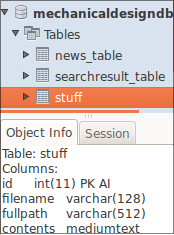
\includegraphics[scale=0.5]{fig/stuffdb.png} 
	\caption{数据库结构}\label{fig:数据库结构} 
	\end{figure}
	
	现在完成了数据库结构的设计,下一步就要用具体的内容来填充它。此处数据库的操作较为简单,就采用了Java自带的JDBC进行文档数据库的添加新数据的操作。大致流程如图\ref{fig:数据库信息写入流程}。
	
	\begin{figure}[htbp] 
	\centering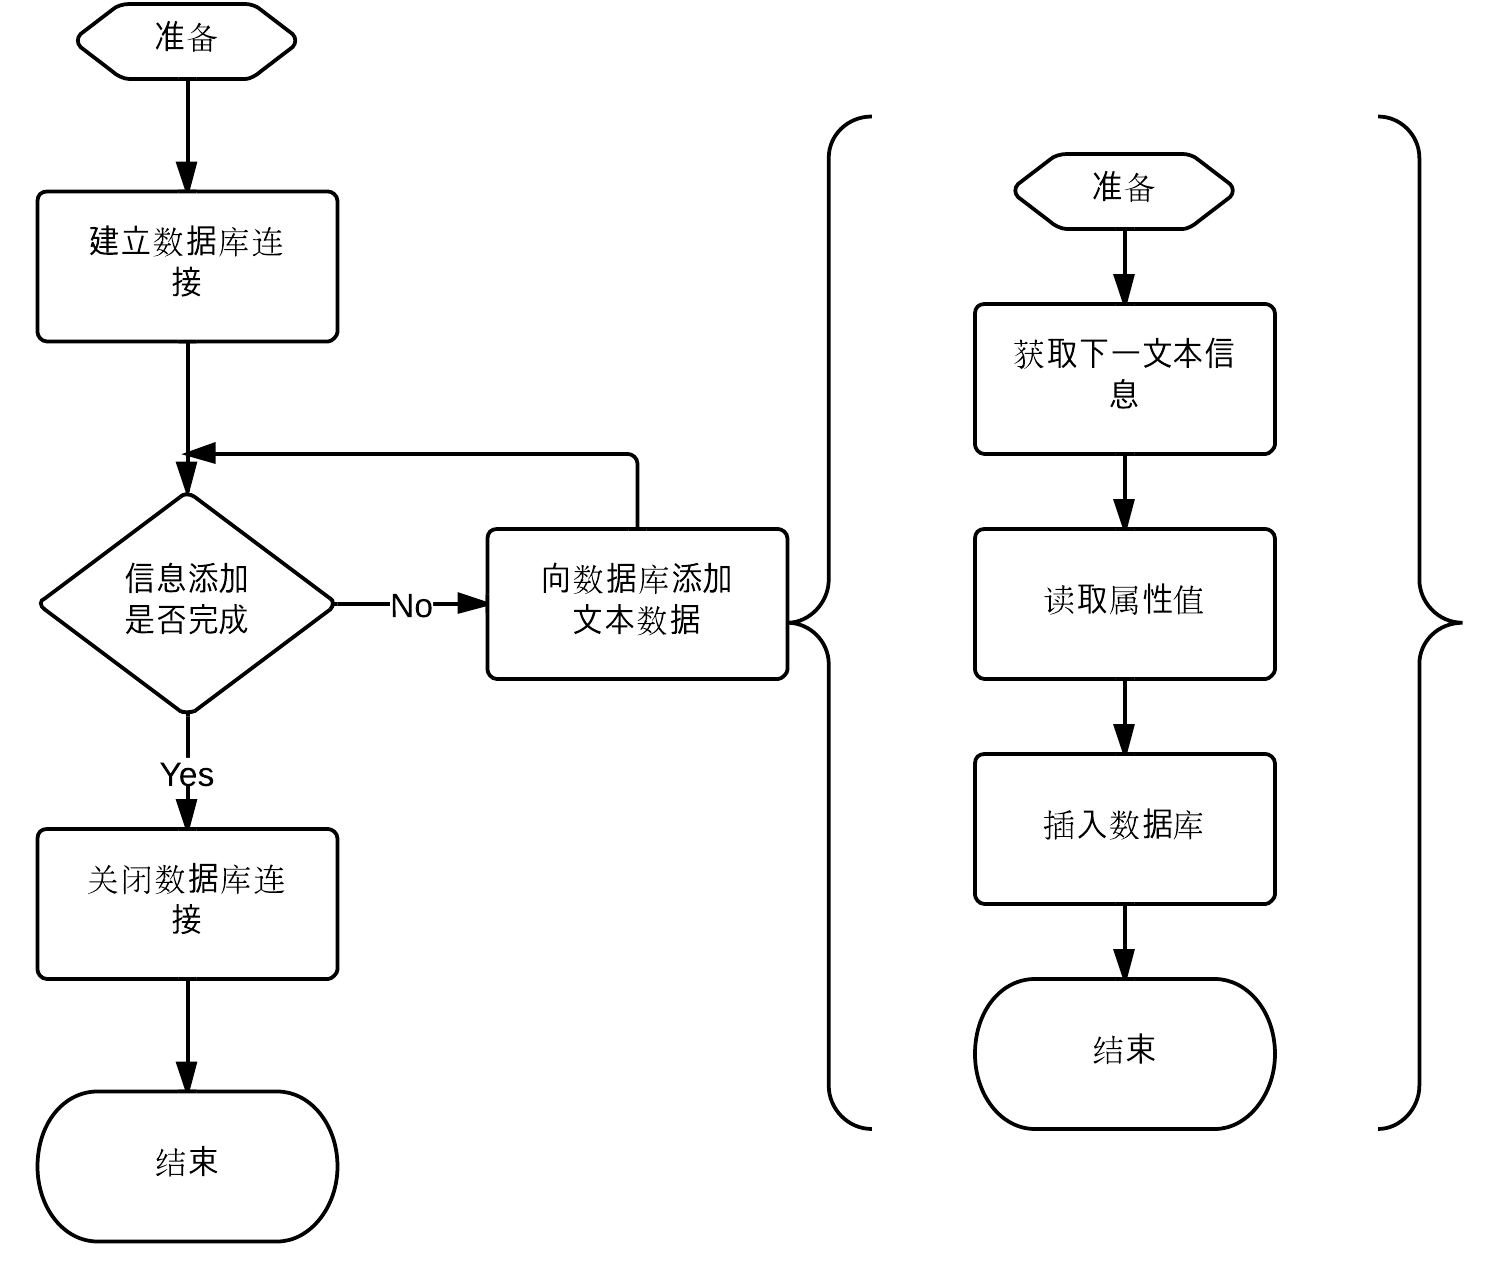
\includegraphics[width=4in]{fig/createdb.png} 
	\caption{数据库信息写入流程}\label{fig:数据库信息写入流程} 
	\end{figure}
	
	JDBC为访问数据库提供了极为方便的接口。
	\lstset{language=Java,frame=lines}
	\begin{lstlisting}
import java.sql.*;
Connection con = DriverManager.getConnection(url, usr, pwd);
	\end{lstlisting}	

	通过引用java.sql包下的相关类,实例化出一个Connection类的对象,以数据库的URL、用户名、密码为参数,调用DriverManager类的静态方法getConnection,就可以实现与数据库的连接。接下来要向数据库中添加信息。用JDBC来操作数据库的核心之一,就是在Java中执行SQL语言,在这儿有必要对SQL语言进行一定的介绍。
	
	SQL(结构化查询语言,Structured Query Language),是用来对数据库进行读写添删等操作的计算机语言,用户不用考虑数据的具体存储方式,只需在高层数据结构上进行操作。SQL的操纵对象是记录项目(records)的集合,所以SQL接受记录项目集为输入,又输出记录项目集,这样一来,SQL语句能够嵌套,从而使他具有极大的灵活性。SQL的一个语句就可以描述相当复杂的查询要求,而要用其他编程语言实现相同的功能,可能需要一段不短的代码。
	
	SQL语句大致被分为两个部分:数据操作语言(DML,Data Manipulation Language)和数据定义语言(DDL,Data Definition Language)。由于篇幅的限制,此处就只介绍本系统中使用到的语言。
	
	数据定义语言是用于实现数据库结构上的操作,比如新建、删除数据表,定义键、字段,规定表格之间的联系等。本系统建立过程中用到的数据定义语言指令有:
\begin{itemize}
	\item
	create database:用于新建数据库
	\item
	create table:用于新建数据表
\end{itemize}		
	
	前面提到了采用SQL语言建立本系统所需要的数据表,大致代码如下:
	
	\lstset{language=SQL,frame=lines}
	\begin{lstlisting}
create database mechanicaldesigndb; --创建数据库
use mechanicaldesigndb; --以该数据库为操作对象
create table stuff; --创建数据表
(
	id int AUTO_INCREMENT, --新建整型的id字段,它具有自增的属性
	filename varchar(128), --新建长度为128字节的字符串型filename字段
	/*
	用类似的方法新建fullpath, content字段
	*/
	primary key(id) --定义id字段为主键
)
	\end{lstlisting}	
	
	这样就完成了数据库及数据表结构上的搭建,这种建立方法是基本不依赖于数据库软件的,也就是说尽管现在系统采用的是MySQL数据库,但是这种方法可以很容易地移植到其他数据库上。下面介绍在数据表内容上的操作方法。
	
	SQL是用于查询数据库的语言,它同时也肩负着插入、删除、更新记录的任务。这些就是由数据操作语言部分来完成,常用的操作指令有:
	
	\begin{itemize}
		\item
	SELECT:用于从数据表中获得数据。
		\item
	INSERT:用于向数据表中添加数据。
	\end{itemize}
	
	在将文档集写进数据库的操作中,id字段并不是文档集中的文档自带的,在数据库中,我们建立了自增的id号,数据库中它可以自行获得,但是如前文所述,这个id将会要作为一个关键参数沟通数据库、索引和网页前端,这就要求从数据库中获得id号,然后把它编入索引当中。这恰就是一个最简单的查询范例。
	
	\lstset{language=SQL,frame=lines}
	\begin{lstlisting}
select max(id)+1 from stuff
	\end{lstlisting}	
	
	简单地解释一下,select语句的语法结构为:SELECT 列名称 FROM 表名称。(SQL语言对大小写不敏感,也就是select和SELECT是完全等效的)。通过这个语句可以获得某个表中的某一列或者几列的数据。列名称所在的位置很灵活的,可以使用通配符“*”来获得所有的列数据,也可以像上面代码这样,在列名称的位置写SQL的内建函数。max()就是SQL的内建函数,用来获得某一列的最大值。通过这个语句就可以获得当前数据库数据条目的数目,再加1,作为下一个条目的id,编进索引的id域中。
	
	完成id字段的操作,下面就需要把文档中的内容导入到数据库中,SQL提供了增加记录项目的语句insert,其语法结构为:INSERT INTO 表名称 VALUES (值1, 值2,....)	或 INSERT INTO table\_{}name (列1, 列2,...) VALUES (值1, 值2,....),可以实现相应的功能。
	
	前面提到,有了JDBC,就可以在Java中执行SQL语句。以上面获得最大id的语句,在java中需要是这样实现的:
	\lstset{language=Java,frame=lines}
	\begin{lstlisting}
Statement pstmt=null; //定义一个Statement类的对象
pstmt = con.prepareStatement("alter table stuff AUTO_INCREMENT 1;");
//把SQL语句作为一个参数传给Connection类对象的prepareStatement()方法
pstmt.execute(); //执行这个Statement类的对象
	\end{lstlisting}	
	
	Statement类是用来执行静态的SQL语句,并返回SQL语句产生的结果。通常情况下,一个Statement类的对象只能获得一个结果集,也就是说,对于不同的结果集,必须要建立不同的Statement类对象。
	
	由于在进行SQL查询时,可能会需要输入不同的参量,Statement类提供了setString方法,以给定的Java字符串来设置SQL语句的参数,驱动器会把Java字符串转换成规模对应的SQL串。举个例子:
		\lstset{language=Java,frame=lines}
	\begin{lstlisting}
//...
String expr =
"insert into stuff (filename, fullpath, contents) values (?,?,?)";

pstmt = con.prepareStatement(expr);
pstmt.setString(1, filename);
//...
	\end{lstlisting}	
	
	这样就可以以之前定的字符串filename作为第一个参数,代替掉第一行最后括号中的第一个问号。通过这样的方法,可以分别获取文件名、文件内容、完整路径信息,并把它们写进数据库。这样就实现了建立文档数据库的功能。
	
	至此,系统体系结构中的资源层已经架设完毕。

		\subsubsection{数据库读取操作}
	上面介绍了用JDBC来实现数据库建立的方法,而对于数据库的操作,还有一个鼎鼎大名的包——Hibernate,也就是最常用的Java Web应用开发架构组合SSH中的那个H(另外两个分别为Spring和Struts 2)。Hibernate是基于JDBC的,它封装了访问数据库的底层细节,因此JDBC具有较强的灵活性,而Hibernate具用较强的易用性和易学性。考虑到搭建这个系统的另一个目的是要熟悉Web应用开发的流程及各种组件,所以在数据库读取操作中,系统采用了Hibernate而非JDBC。
	
	目前流行的编程语言,Java、C++等都是面向对象的,但是主流的数据库产品又还是关系数据库\cite{li2008}。这两者发展由于理念上的差异,造成发展不协调,也就催生了ORM(Object/Relation Mapping)框架来沟通连接这两者,通过ORM框架,应用程序就不用直接访问底层数据库。Hibernate就是ORM框架中较为常用的一种。Hibernate是由JBOSS提供的一套开源的对象关系映射框架,通过对JDBC进行封装,其最大的特点就是把数据库当作一个对象,因此可以用面向对象的思维来操纵数据库,这些对数据库的操作将会被ORM解析成SQL操作,从而避开了一些有时冗长艰涩的SQL语言,数据结果也从数据表的表现形式变成了对象的形式,这对于那些采用面向对象的业务模性和商业逻辑的应用是有利的。
	
	对于ORM框架,有一个非常重要的媒介——PO(持久化对象,Persistent Object)。正是通过PO才能完成持久化操作,也就是前面所说的以面向对象的方式来操纵数据库。在Hibernate中PO是很简单的:

	$$ PO = POJO + 映射文件 $$

	其中POJO是指普通Java类,由于Hibernate的低浸入式设计,POJO类与普通JavaBeans是一样的,它不要求持久化类继承什么父类或是实现什么接口。Hibernate中的映射文件以XML的形式书写,通过映射文件,Hibernate就可以理解持久化类和数据表之间的关系,也可以理解持久化类属性与数据表列之间的关系。以本搜索系统的使用为例:
	
\lstset{language=XML,frame=lines}
\begin{lstlisting}
<hibernate-mapping package="myPackage">
 <class name="SearchResult" table="stuff">
  <id name="id">
   <generator class="identity"/>
  </id>
  <property name="contents"/>
  <property name="filename"/>
  <property name="fullpath"/>
 </class>
</hibernate-mapping>
\end{lstlisting}	

	上面的映射文件中定义的property的name与POJO类中一一对应。这样一样就实现了持久化对象。接下来通过Hibernate配置文件hibernate.cfg.xml,配置出数据库的类型、URL、用户名、密码,以及映射文件的路径,就完成了Hibernate的前期配置工作。可以开始利用Hibernate来操作数据库了。
	
	回顾一下搜索系统工作流程,系统接受用户的查询请求,通过语义扩展生成了新的请求,以它在索引中搜索,获得了结果文本的ID号,然后通过这个ID号获得搜索结果的具体内容。那么用Hibernate要实现的功能就是要通过ID号在数据库中找到该ID号对应项的其他字段的信息。根据Hibernate的框架规范,建立一个包含id、 contents、 filename、 fullpath的POJO类SearchResult,其形式是JavaBean。按照上面的映射文件,进行映射配置。接下来建立通过ID查内容的方法:
	
\lstset{language=Java,frame=lines}
\begin{lstlisting}
public static SearchResult findStuffById(String id){
 Session sess = HibernateUtil.currentSession();
 //开始事务
 Transaction tx = sess.beginTransaction();
 //创建消息实例
 List pl =sess.
 	createQuery("select stuff from SearchResult as stuff where id = :id")
 	.setString("id", id).list();
 //通过id号获得数据库中该id号对应的记录
 Iterator pit = pl.iterator();
 //用迭代器来获得List类里的信息
 SearchResult s = (SearchResult)pit.next();
 //以SearchResult类保存查询结果,
 tx.commit();
 //提交事务
 HibernateUtil.closeSession();
 //关闭事务
 return s;
}
\end{lstlisting}	

	这样一来,用id号获得的数据库中的记录就变成了一个SearchResult类的对象,这样一来“findStuffByID("1").getfilename”就可以获得id号为1的记录中文件名信息。这对于之后网页前端的显示来说是极为方便的。
	
	到这里,系统体系结构中的应用服务层也搭建完毕,通过Jena、Hibernate、JDBC等包,实现了与资源层的信息交互,完成了扩展性语义搜索、索引器、数据库维护器等功能集的设计与制作,后台已经准备好,下面就要考虑设计前端,使用户可以通过它,与后台打交道,获得相对应的服务。

	\subsection{服务器架设}
	
	在系统设计之初,我们就把它定位成能够跨平台的搜索系统,一个Web应用程序恰能较简单地实现这样的功能。什么是Web应用程序呢?
	
	所谓Web应用程序是一种可以通过Web访问的应用程序,其优势在于用户不需要安装其他软件,只需在浏览器中即可访问应用程序。
	
	传统的应用程序是被完全部署在一台计算机上的,就像早期的单机游戏,只要通过光盘安装在了本地的计算机,你不需要与其他电脑产生任何联系,就可以完美地运行。但是随着互联网的迅速发展,人们已经不在满足于局限在一台计算机上的资源,而希望使用其他计算机的信息和资源,这就催生了Web应用程序。
	
	与传统的应用程序不同,现在的很多应用程序可能并不是被部署在一台计算机上,或者说应用程序所在的计算机可能与调用该应用程序的计算机不同。这种应用程序至少与两台计算机发生了关系,所以就产生了两种不同的架构:B/S架构,即浏览器(Browser)/服务器(Server)架构,与此相对应的还有C/S架构,即客户端(Client)/服务器(Server)架构。两种架构都涉及了S端,即服务器端,从字面上说,它是提供服务的机器,因为它可能需要同时给多个浏览器(或客户端)提供服务,所以要求服务器端计算机拥有较好的性能。下面再来看看两种架构的不同点,对于B/S架构,它是从浏览器中获得服务器的服务的,这样一来,只要有一个浏览器,你就可以享受到不同服务器提供的不同服务;对于C/S架构,需要在C端,即客户端部署程序,这个程序可以自己完成一些任务,也可以与服务器进行信息的交互。这样我们看出,对于B/S架构,在浏览器中几乎是只发出服务请求,而很少承担完成服务所需要的工作,比如对于一个聊天室,浏览器端完成的只是发送信息到服务器,再从服务器上获取信息这样的简单的工作;相对应的,对于C/S架构,客户端就会承担完成服务的较多工作(相比较B/S架构而言),这一方面是受到服务器端计算机性能的限制,另一方面也是受到网络传输的限制,所以在客户端就需要部署相应的较为复杂的程序,而这个程序不能简单地放在浏览器中来完成,比如对于一个大型网游,画面的渲染就是一个计算量颇大的任务,如果把这些工作都交给服务器来完成,可能服务器吃不消,可能网络传输速度的限制就让你根本无法足够迅速的传送渲染的请求并接收服务器端的渲染结果。所以这种架构其实是在平衡远程计算机和本地计算机的负载。
	
	针对我们的搜索系统,用户所需要的信息只是搜索体系的资源层中的小小一部分,所以把整个资源层放在本地计算机上是相当不划算的,但是整个搜索系统又都依托于资源层。这样一来,要完成一个搜索任务,本地计算机能完成的工作是极其有限的,几乎所有的业务逻辑都要在服务器端来实现。所以我们采用了B/S架构建立了一个Web应用程序,这样一来通过通用的浏览器就可以访问搜索系统,而不用在本地安装其他软件,很容易就实现了应用的跨平台性。
	
	上面多次提到服务器,那么什么才是服务器呢?根据全国科学技术名词审定委员会定义,服务器是指一种运行管理软件以控制对网络或网络资源(磁盘驱动器、打印机等)进行访问的计算机,并能够为在网络上的计算机提供资源使其犹如工作站那样地进行操作。那么归根结底,服务器也是一种计算机,只是性能上会优于普通的个人计算机,那么它是依靠什么机制来让它成为可以提供服务的服务器而不是一般计算机的呢?是Web服务器。需要与之前说的服务器相区分的是,之前说的服务器是硬件,是一台性能优越的计算机;而Web服务器是程序,它可以接收浏览器发出的请求,并做出回应,给出漂亮网页作为结果,当然它不只能提供静态的HTML网页,还可以运行程序来响应用户的请求。
	
	由此可见,通过Web服务器,普通的个人电脑也可以充当服务器。之前我们提到了搜索系统采用B/S架构,那么这种架构会涉及到两端:服务器端和浏览器端。而正是Web服务器,将该计算机的一部分作为服务器,再用同一台计算机(当然对于其他计算机也是相同的)的浏览器访问这个服务器,获得相关服务,这样一来就让一台电脑分饰两角了。
	
	常用的Web服务器软件有Tomcat、Apache和Microsoft的Internet信息服务器(Internet Information Server,IIS)。

		\subsubsection{Tomcat}
	Tomcat是Apache软件基金会的一个开源项目,它是一个Web服务器,也是一个Java servlet容器(container),与此同时,它还提供了Java servlet和JSP(JavaServer Pages)技术。Tomcat作为一个开源优秀的项目,吸引了众多编程高手加入其中,它使用先进的技术,性能稳定,而且免费,常被Java程序员使用。它属于轻量级服务器,被广泛用在中小型系统和并发用户不是很多的情况,是目前一种较为流行的Web服务器。结合本系统的需求,本系统采用Tomcat作为服务器。架设Web服务器的常见操作系统有Linux,Windows和Unix,其中Linux可以支持多个硬件平台,网络功能较为强大,是架构高效安全的Web服务器的理想选择。我们选择Linux的Ubuntu版本作为Web服务器架设平台。
	
	下面简要介绍一下在Linux下的Tomcat的配置方法:
	
	\begin{enumerate}
		\item 配置Java编译环境:因为Tomcat是基于Java的,要运行Tomcat首先需要配置Java编译环境,其步骤大概是从Java官方网站上获得jdk包,解压并安装在本地硬盘,设置环境变量,最后可以通过“java -version”命令查询jdk的版本从而了解Java编译环境的配置情况。
		\item 安装Tomcat包:从Tomcat官方网站上可以获得Tomcat安装包,下载解压到本地。
		\item 配置Tomcat:Tomcat的配置主要是三个方面:系统环境、server.xml、tomcat-users.xml。对于系统环境部分,要在环境变量中配置CATALINA\_{}HOME和CATALINA\_{}BASE的路径,这样才能保证Tomcat在执行它的命令的时候,能知道这些命令在哪儿。通过server.xml可以配制catalina的端口号,默认情况是8080,但在一些罕见的情况下,这个端口号可能冲突。通过tomcat-users.xml主要存储了tomcat的用户设置,包括用户名、密码、用户类别等。
		\item 运行Tomcat:运行startup.sh就可以运行Tomcat,打开浏览器,访问“http://localhost:8080/”,如果能看到如图\ref{fig:Tomcat服务器配置成功}界面,则Tomcat配置成功。
	\begin{figure}[htbp] 
	\centering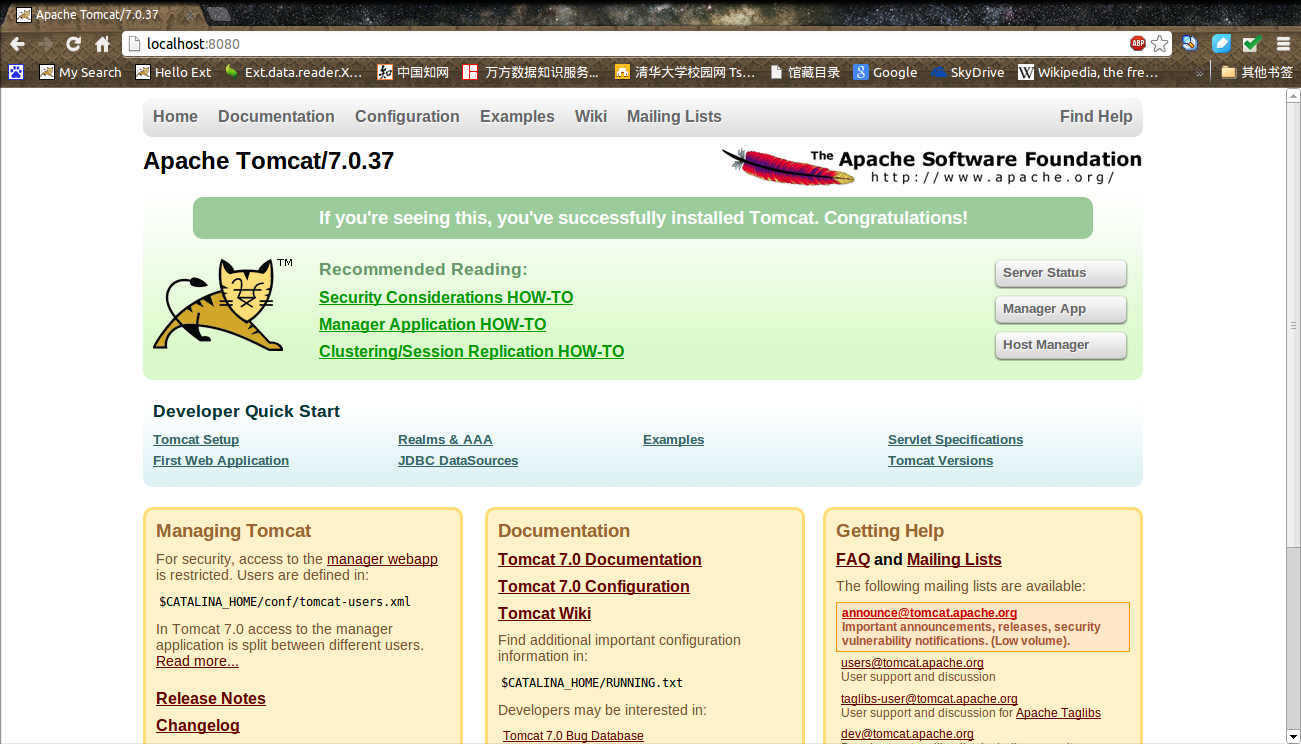
\includegraphics[width=4in]{fig/tomcatsuccess.png} 
	\caption{Tomcat服务器配置成功页面}\label{fig:Tomcat服务器配置成功} 
	\end{figure} 
	\end{enumerate}
	
	现在完成了Tomcat的配置,建立好Web应用程序,把它部署到Tomcat中,就能通过浏览器来访问它了。
	
	Tomcat位于显示层,是沟通用户与系统后台的关键机制。它作为一个容器,装载了包括JSP网页,实现了用户访问、发送请求、返回结果、显示结果的功能。
		
	\subsection{前端设计与实现}
	有了Tomcat这个容器,下面就要编写容器里面的内容,一方面实现功能的可视化操作,另一方面,实现查询业务逻辑。用户与系统的沟通,归结来说就是一组请求(Request)和响应(Response),即用户发给系统响应,系统通过调用后台的Java类,计算出相应的结果,然后返回给用户一个响应。要实现这样的机制,可以采用一些现成的框架,比如DWR、Struts2。
	
	DWR(Direct Web Remoting)是一个便于实现web页面与Java类交互的远程服务器端Ajax开源框架,通过把Java类虚拟映射成为JavaScript程序,在浏览器中就可以方便地调用Java类。在系统搭建过程中,我们也尝试了采用这种框架,但是ExtJS与它的兼容性问题一直没有得到解决。
	
	Struts2也可以通过拦截器机制实现类似功能,但是它配置较为复杂。相对于本系统较为简单的逻辑关系,就不采用这种架构,而直接用一个JSP来处理用户发送的请求,事实上,这种处理方式也是模仿了Struts2的流程,但是由于自定义的JSP针对性更强,所以大大减少了功能实现的时间和空间成本。于是得出了搜索引擎传统Web服务模式,如图\ref{fig:搜索引擎传统Web服务模式}。
	\begin{figure}[htbp] 
	\centering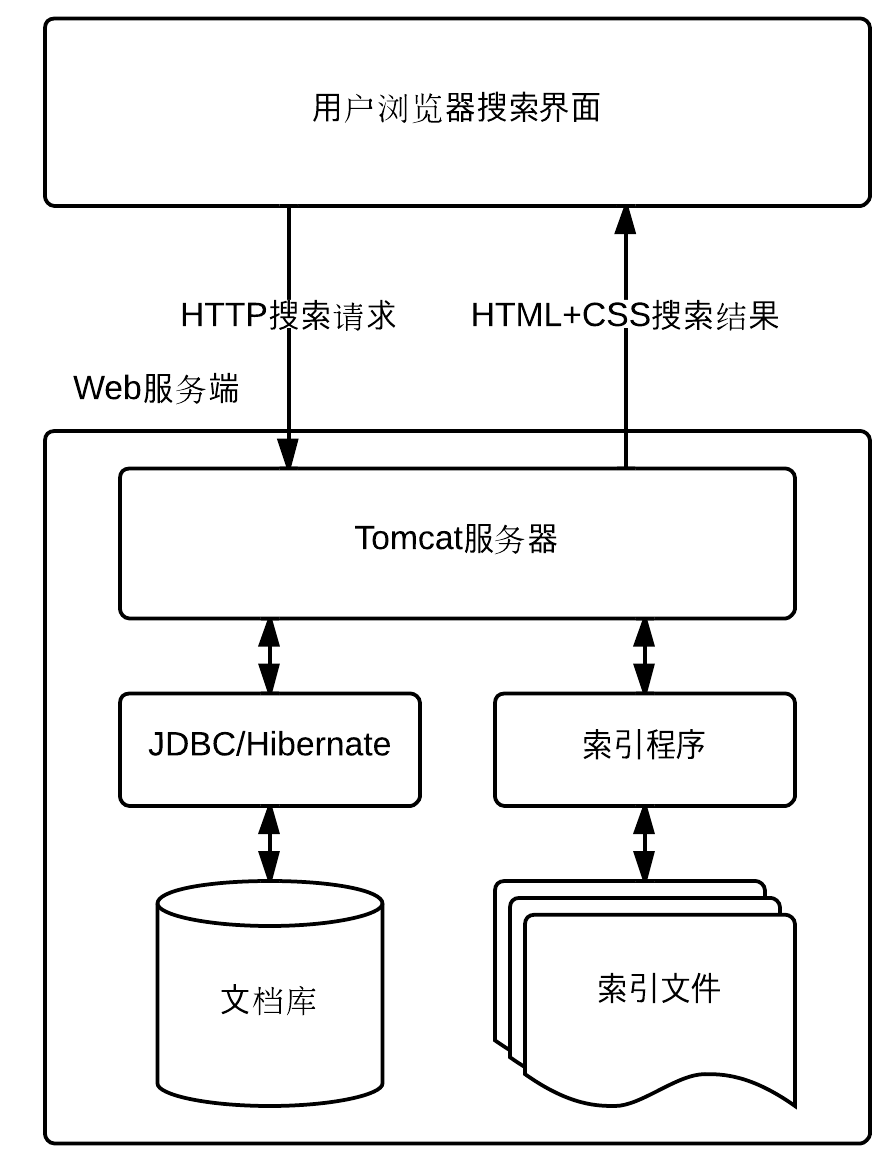
\includegraphics[width=3in]{fig/SearchStructure.png} 
	\caption{搜索引擎传统Web服务模式}\label{fig:搜索引擎传统Web服务模式} 
	\end{figure} 
	
	通过这样的流程,把用户的查询词条封装在请求中,通过一个充当Servlet的JSP网页,解析这个请求,把查询词条作为Java搜索类的参数,进行搜索,获得相应的文件号,再将其封装成响应,返回到客户端,客户端的前端将其解析,并显示出来,从而实现了系统的搜索逻辑。
	
	编写网页前端的方法有很多,包括最基本的HTML和CSS,以及JavaScript。按照一般的方法,HTML主要负责定义元素,CSS进行网页风格的设计,JavaScript实现效果和交互。在JavaScript进行效果和交互的环节可以采用jQuery,它是JavaScript框架,能够方便地处理HTML元素,实现动画效果。ExtJS是jQuery更高层的封装,系统采用ExtJS来编写用户界面,下面就ExtJS进行简单的介绍。
		
		\subsubsection{ExtJS}
	ExtJS是一种基本摆脱了后台技术的前端ajax框架,主要用于创建前端用户界面。它的界面风格简约而美观,强大的表格控件为它吸引了大批使用者,因而产生了相当丰富的参考学习资料。ExtJS为编程者提供了极为丰富的组件,下面只介绍本系统使用到的一些组件。
	
	在JavaScript中,当DOM结构准备完毕、图片和影片等资源下载之前,浏览器会触发一个load事件。ExtJS需要一个执行的起点,保证在load事件触发时被调用,这就是:
\lstset{language=C,frame=lines}
\begin{lstlisting}
Ext.ready(function(){
//程序体
});
\end{lstlisting}	

	下面的各种组件,都将被嵌在上述结构中。
\begin{enumerate}
\item
Viewport容器:

	为了界面美观整洁,需要将页面进行区域划分,不同的区域安放不同的控件。比如在我们的页面中,上方为搜索栏,左侧为扩展词表/文件列表,中间为搜索结果摘要,右侧为文本全为显示,下方为搜索系统说明。Viewport就提供了这样的功能,它首先占据整个页面,再将页面分成5大区域:north, west, center, east, south,以此对应上、左、中、右、下。有了Viewport这个容器,就可以将其他的Panel等控件放在相对应的位置,保证了页面的结构。
	
\item
Panel容器:

	Panel容器是一个面板,它同样可以装载各种组件,在系统中,为了保证系统的美观,用Panel容器来进行HTML的直接显示,这样的好处在于,可以直接使用CSS方式标记的高亮部分得以顺利地显示。
	
\item 
GridPanel:

	GridPanel以MVC的模式进行设计,将数据的模型、显示、控制分开处理。Column元素定义了表格中数据的模型,然后用Store来进行数据的读取和存储,把Store读取到的数据转换成Record数组,与Column定义的模型进行映射,每条Record都包含Column模型中的各字段。

\item
FormPanel表单容器:

	FormPanel的功能在于,除了可作为容器装载组件以外,还可以在原有的DOM结构后加上<form/>标记。即FormPanel可以被分作两个部分,一个部分就像普通Panel那样装载组件,另一个部分是实现了数据的存储和表单的提交。
	
\end{enumerate}

	与普通HTML相对应的,ExtJS还提供了文本框,按钮等基本组件。通过他们的合理安排,就可以编写出一个ExtJS风格的用户界面。但是若只到此,页面徒有其表,并不具备处理工作的能力。所以,还需要对相对应的组件添加相应的事件。目前系统需要处理的有两个事件,一个是在文本框中输入了关键词,点击搜索之后,要能进行搜索操作;另一个是在文件列表中点击了某一个文件后,要在全文窗口显示出该文本的内容。
	
	针对第一个问题,将文本框和按钮放在一个表单容器FormPanel中,当在文本框中输入了查询词条,点击搜索之后,将会把文本框中的内容包在一个请求(Request)中发到服务器上的Servlet(JSP实现)中,Servlet通过调用相关的Java类,获得Json格式的搜索结果,其中包括扩展词汇和扩展词汇与中心词汇的关系,带有高亮标签的查询结果HTML文本,以及查询结果文本的ID号,然后把这个Json格式的结果再打包成一个响应,返回到发送请求的页面,页面解析响应中的搜索结果,分别存储以上三种结果,然后在相对就的控件中,显示这些结果。
	
	针对第二个问题,把文件名列表的GridPanel增加一个监听器(Listener),负责监听项目点击(itemclick)操作,当用户点击了某个项目,就会利用ExtJS的Ajax包中的Request组件,把之前获得的搜索结果文件ID号打包成响应,发送到另一个用JSP实现的Servlet,它会从根据ID号,从数据库中得到相对应的文档内容,再打包在响应中,返回响应页面,加载到文本全文的容器中。
	
	这样,就可以实现前端页面,以及前端页面和后台Java类的交互。	

		\subsubsection{用户界面编写}
		通过以上组件的组合,就获得了如下的用户界面,如图\ref{fig:用户界面}。
	\begin{figure}[htbp] 
	\centering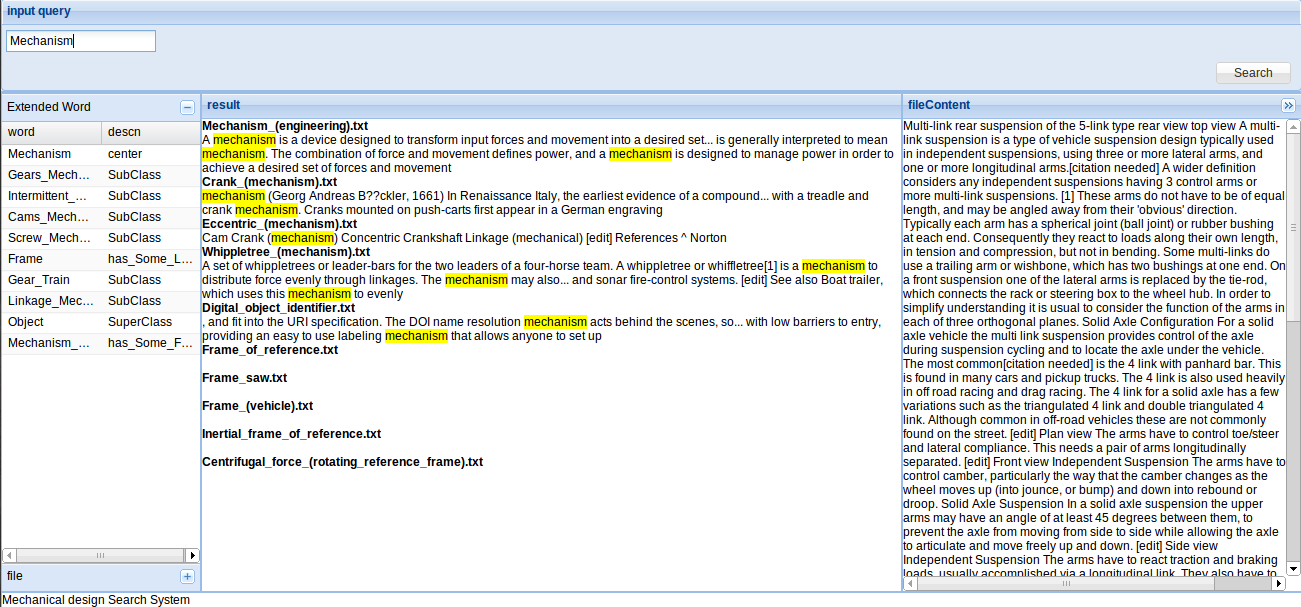
\includegraphics[width=6in]{fig/GUI.png} 
	\caption{用户界面}\label{fig:用户界面} 
	\end{figure} 
		
	在input query表单中输入查询词条,点击Search,在Extend Word中就会显示出相应的扩展词汇,以及查询词条与这些词之间的关系。在result中将会显示搜索结果的摘要文本,并且能够高亮显示用户输入的查询词条,更直观地显示出查询结果的相关度。打开“手风琴”效果的file面板,就可以看到查询结果对应的文件名列表,点击其中任一个文件,在fileContent面板中,就能够显示相应的文本全文。
	
	至此,就完成了整个搜索系统的搭建,并实现了相应的扩展性语言搜索算法。
	
\newpage
\section{系统实现}
\setcounter{figure}{0}
\setcounter{table}{0}
\setcounter{equation}{0}
	由于本系统是一个软件系统,所以本部分将以软件工程的开发模式,分需求分析、概要设计、详细设计三个部分,对整个系统进行一定的疏理。最后进行查准率、查全率的实验,评估出系统性能。
	\subsection{需求分析}
		\subsubsection{任务概述}
	计算机技术促进了制造技术的发展,制造技术也从一开始指设计制造的狭义概念,发展到现在从采购、生产,一直延伸到销售、售后的广义概念。对于这样产品的制造全生命周期,就会产生海量领域内技术文档,它包括了设计需求报告、设计说明书、设计图纸、加工工艺规程、质量检验报告、维修报告等文档。如何从这些海量的文档中,搜索出我们想要的内容,是企业对市场变化进行迅速的反应的先决条件。
	
	捕捉查询意图的机械领域知识检索系统正是为此目的而设计,它以机械领域的领域本体为知识载体,运用扩展性语义搜索算法,使用户通过较短的查询请求,就可以获得符合其查询意图的结果,根据相关性的排序,将相关度高的文档往前排序,节约用户检验文本的时间,从而提高了搜索效率。
   
		\subsubsection{功能需求}
	要实现一个搜索系统,首先需要一个核心的搜索引擎进行搜索操作;为了实现快速的搜索,需要就文本进行索引	操作,所以需要定制一个专门的索引器;为了存储和调用文档,需要以数据库的方式来组织这些材料,并对它们进行维护操作。由此,得出整体用例图,如图\ref{fig:整体用例图}。
	
	\begin{figure}[htbp] 
	\centering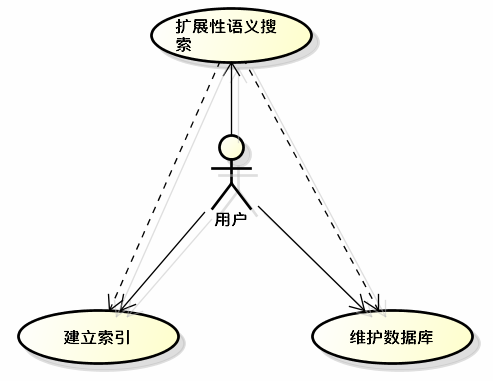
\includegraphics[scale=0.5]{fig/SystemUseCase.png} 
	\caption{整体用例图}\label{fig:整体用例图} 
	\end{figure} 
	
	根据这样的需求,捕捉查询意图的机械领域知识检索系统被分成三个应用功能模块:扩展性语义搜索,索引器,数据库维护器。下面对几个模块分别进行阐述。
	\begin{enumerate}
	\item 扩展性语义搜索
	
	对于一个搜索系统,用户输入关键词,系统返回相应的搜索结果,是其必需的功能。搜索结果应该包含文本的摘要信息,从而给用户提供参考。为了体现语义扩展性,给用户提供思路上的拓展,还应列举出与用户输入关键词相关的概念,并且说明这些概念与关键词的关系。作为一个面向文本搜索的系统,还应该提供文本的全文查看功能。同时,为了实现搜索系统的性能调试,还应该提供改变系统参数的方法。根据这些需求,画出扩展性语义搜索模块的用例图,如图\ref{fig:扩展性语义搜索用例图} 。
	
	\begin{figure}[htbp] 
	\centering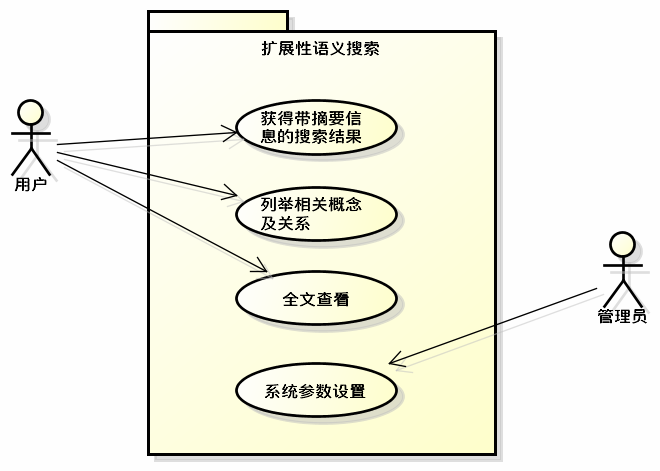
\includegraphics[scale=0.4]{fig/SearchSystemUseCase.png} 
	\caption{扩展性语义搜索用例图}\label{fig:扩展性语义搜索用例图} 
	\end{figure} 

	总结起来,扩展性语义搜索模块应该包含基本搜索,相关概念显示,全文显示,系统参数调整等功能。
	
	\item 索引器
	
	要实现搜索功能,就需要为被搜索的文本进行索引操作,通过索引操作获得索引文件,以一种高效的数据结构,实现快速根据关键词找到相应的结果。所以需要一个索引器,它应该具有对于索引的一般性操作,增加索引、修改索引、删除索引。当然这些操作不面向普通用户,只面向管理员。由此得出索引器模块的用例图,如图\ref{fig:索引器用例图}。
	
	\begin{figure}[htbp] 
	\centering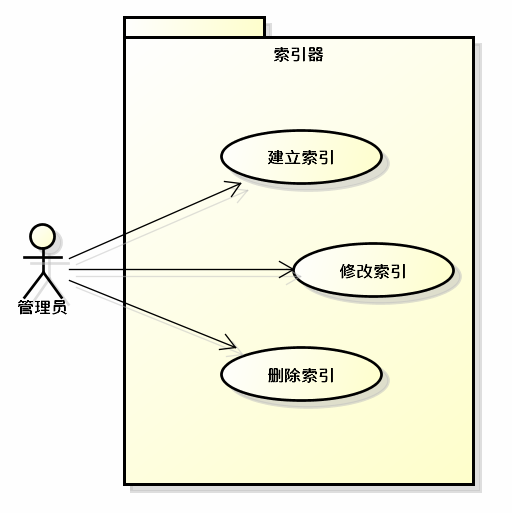
\includegraphics[scale=0.4]{fig/IndexerUseCase.png} 
	\caption{索引器用例图}\label{fig:索引器用例图} 
	\end{figure} 
	
	\item 数据库维护器
	
	为了便于文档的管理,采用数据库的形式来存储文档。如何把普通的文本保存在数据库中?这就需要数据库维护器,它将完成数据库的基本操作,包括面向管理员的数据库记录的新建、修改、删除操作,以及面向用户的数据库记录的读取等操作,由此得出数据库维护器用例图,如图\ref{fig:数据库维护器用例图}。
	
	
	\begin{figure}[htbp] 
	\centering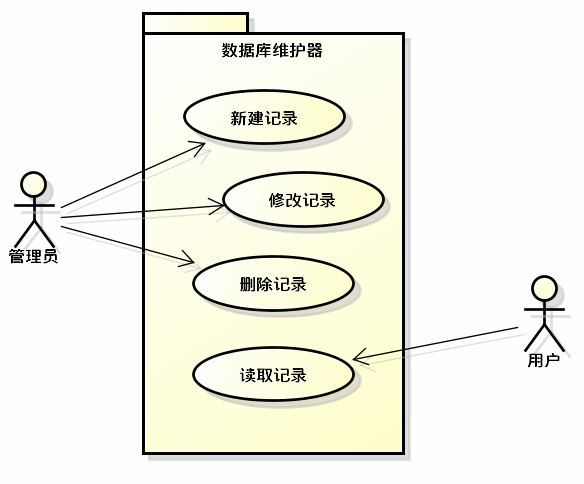
\includegraphics[scale=0.4]{fig/DatabaseUseCase.png} 
	\caption{数据库维护器用例图}\label{fig:数据库维护器用例图} 
	\end{figure} 
		
	\end{enumerate}
		\subsubsection{运行需求}
\begin{itemize}
	\item
	服务器端软、硬件要求:
	\begin{enumerate}
	\item
	硬件要求:
	
	Pentium IV以上处理器,512M以上内存,80G以上硬盘空间
	
	\item
	软件要求:
	
	系统软件:Linux(Ubuntu 12.04 LTS)
	
	Web服务器:Apache Tomcat 7.0
	
	数据库:MySQL
	
	其他:jdk1.7
	\end{enumerate}
	
	\item
	客户端软、硬件要求
	\begin{enumerate}
	\item
	硬件要求:
	
	Pentium IV以上或相同性能的其他CPU,32M以上内存,4G以上硬盘空间。
	
	\item
	软件要求:
	
	系统软件:Windows 2000以上, OS,IOS, Android多平台支持
	
	浏览器:Internet Explorer、Firefox、Opera、Chrome、Safari多种浏览器支持
	\end{enumerate}
	
\end{itemize}
		
		\subsubsection{运行需求}	
		
\begin{enumerate}
\item 用户界面
结合之前的功能需求分析,用户界面是基于Web浏览器,大致分为以下几个部分:搜索框,扩展词列表,相关文件列表,搜索结果显示,全文显示,如图\ref{fig:页面布局图}。

	\begin{figure}[htbp] 
	\centering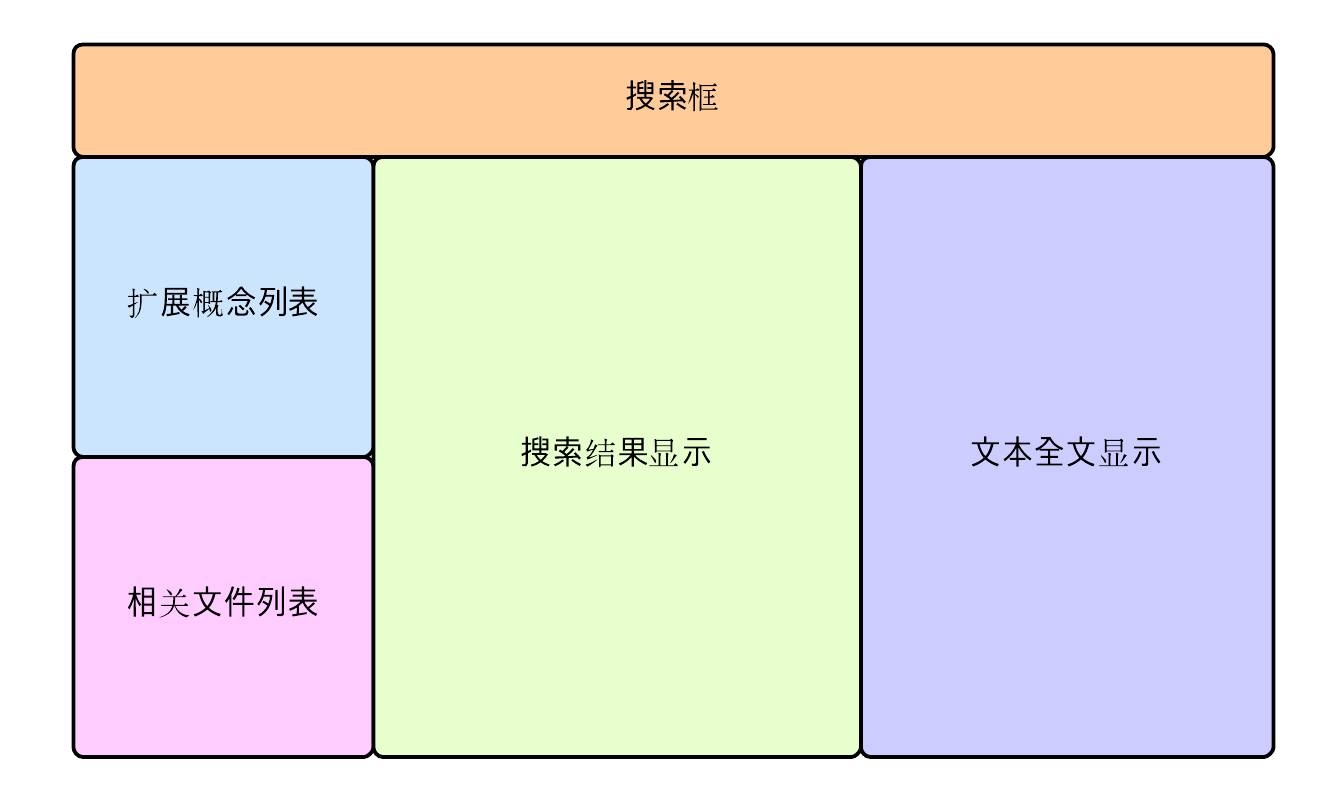
\includegraphics[width=4in]{fig/WindowsDistribution.png} 
	\caption{页面布局图}\label{fig:页面布局图}
	\end{figure} 

\item 软件接口
系统要尽量采用MVC结构来构建,将模型、视图、控制分开,让系统更利于维护。使得各功能模块具有各自独立的功能,具有丰富实用的接口,松散地耦合成一个整体。

\item 故障处理
要利用Chrome,Firefox等浏览器的网页调试功能,在系统运行的关键节点,发送相关的调试信息,便于故障的处理。
	
\end{enumerate}		
		
		\subsubsection{其他需求}
	由于扩展性语义搜索是一种基于知识的搜索算法,所以需要选用一种知识的表达方式,并采用扩展性好的软件进行知识的建模。
	
	\subsection{概要设计}
		\subsubsection{基本处理流程}
	
	根据B/S架构Web应用的相关协议,作出相应的客户端与服务器端交互的时序图,如图\ref{fig:B/S交互时序图}。
	
	\begin{figure}[htbp] 
	\centering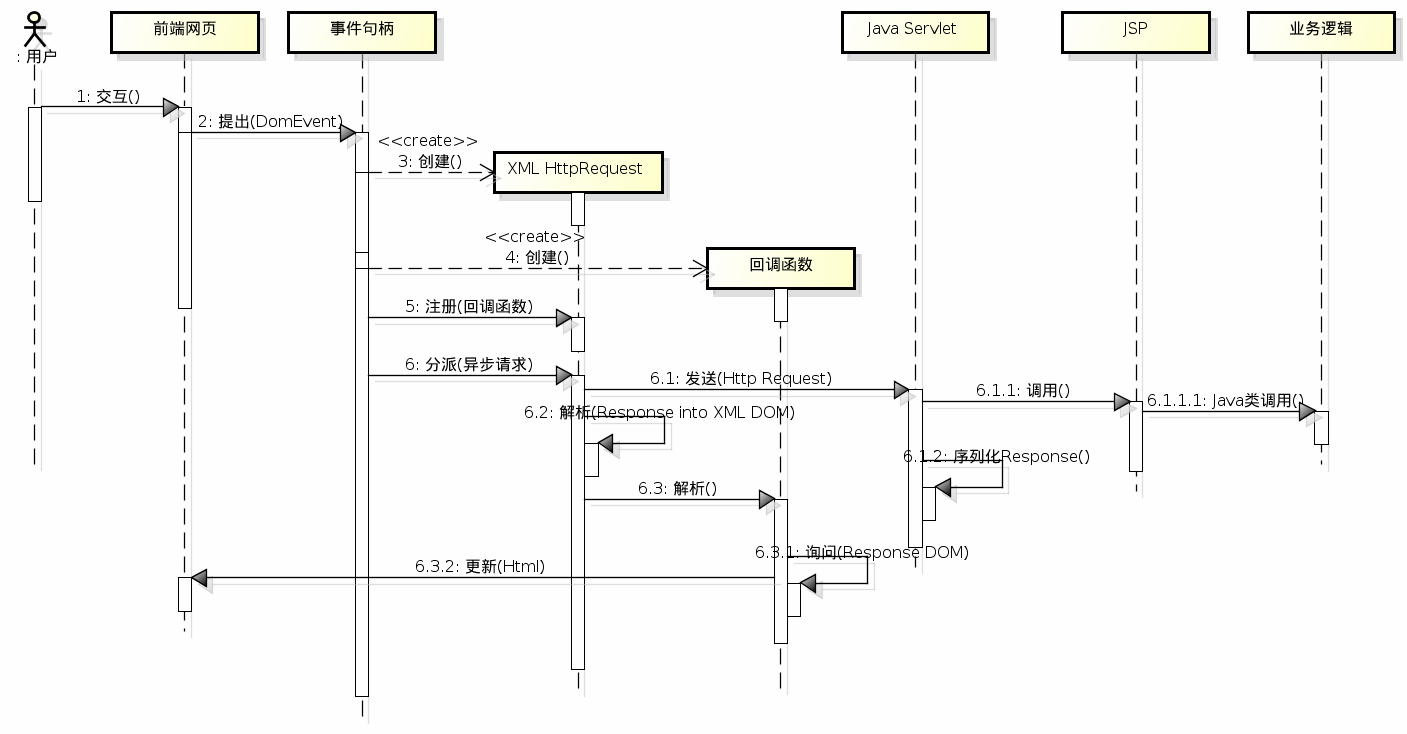
\includegraphics[width=5in]{fig/Sequence.png} 
	\caption{B/S交互时序图}\label{fig:B/S交互时序图}
	\end{figure} 
	
	具体到业务逻辑,可以得出后台搜索时序图,如图\ref{fig:搜索时序图}。
	
	\begin{figure}[htbp] 
	\centering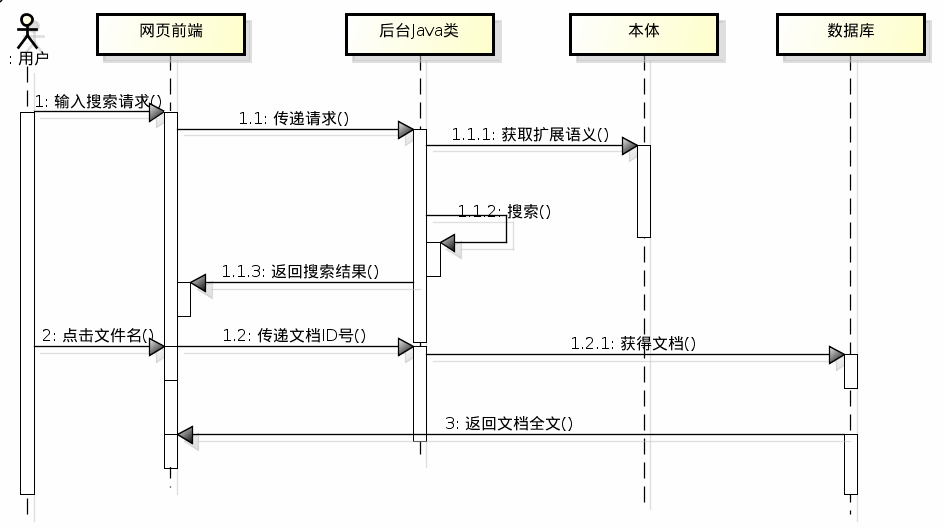
\includegraphics[width=5in]{fig/SearchSequence.png} 
	\caption{搜索时序图}\label{fig:搜索时序图} 
	\end{figure}
	
	首先,用户在前端网页中输入搜索请求,前端网页将请求传递到后台Java类中,Java类通过读取本体,获得了扩展语义,然后进行搜索,返回相应的结果,包括高亮的摘要结果、扩展词汇及关系、搜索结果的文件名;当用户点击某个文件名后,前端网页会通过文件对应的ID号,调用数据库中的相关记录,并呈现在前端网页中。从而实现搜索功能。
		
		\subsubsection{组织结构}
	系统组织结构如图\ref{fig:体系结构},自下而上分为资源层,应用服务层,表示层,客户端层。
\begin{itemize}
	 	\item
	资源层:资源层为检索系统提供了有组织的文档库,它是通过爬早程序从互联网上获得的文档,通过解析操作,去掉了HTML标签,转化为非结构化文本,将其组织在数据库中,作为被搜索的文本;提供了领域本体,本体的建立结合了人的认识规律,按照本科教学的学习培养方案,将《机械原理教程》《机械设计教程》进行一定的简化和概括,再按照一定的本体构建规则,以本体形式录入,作为扩展性语义搜索算法的基础;提供了本体的实例层,为实例搜索提供数据源,同时,由于本体的推理功能是在实例层进行的,所以为实现推理功能,而不是单纯的扩展功能,需要将一些重要概念进行实例化,从而更好地利用了本体的另一强大功能。
		\item
	应用服务层:应用服务层主要包括两个部分:Java工具包层,提供Jena、Lucene、Hibernate等工具包,Jena实现了本体的读取操作、Lucene实现文档库索引与搜索功能、Hibernate实现操作数据库的功能。这些工具包强大而灵活,为系统开发提供了极大的便利,缩短了开发周期。该层也是连接应用服务层与资源层的枢纽层。
	
	功能集层:这是检索系统的核心部分,提供扩展性语义搜索功能,索引器功能和数据库维护器功能。索引器可以对特定目录的文档创建索引,数据库维护器可以把这些文档加入到搜索数据库中,从而实现了知识库维护功能,将本体、知识库、扩展性语义搜索算法松散耦合地集成在一起,同时提供灵活丰富的接口,保证与表示层的正常通讯,同时为今后功能扩展提供支持。
		\item
	表示层:在表示层内采用开源泉的Tomcat容器架设服务器,采用B/S架构,在服务器端完成大部分业务逻辑,减轻客户端负载。采用Javascript和ExtJS库编写用户界面,可以相对容易地实现美观友好的用户界面,使用户便于使用系统提供的功能集。这样,就保证了系统的跨平台性。
		\item
	客户端层:客户端层为用户终端,由于系统采用了B/S架构,用户无需安装客户端软件,只需像登录普通网页那样,登录检索系统网页,就可以使用系统各项功能。系统逻辑主要由部署在服务器端的程序完成,这样也就使对客户端层的设备配置要求低,保证了系统的跨平台性。由于对移动平台的兼容性,可以让设计人员在任何时候都能方便地查询所需要的设计知识,符合了“随时随地设计”的理念。
	
	\end{itemize}
	
		\subsubsection{模块划分与接口设计}
	根据模块划分高内聚,低耦合的特点,结合图\ref{fig:体系结构}的系统组织结构图。又将资源层和应用层结构进行进一步地细分。并描述它们之间的联系关系,定义必需的接口,为后面的详细设计提供参考,如图\ref{fig:模块与接口设计图}。
	
	\begin{figure}[htbp] 
	\centering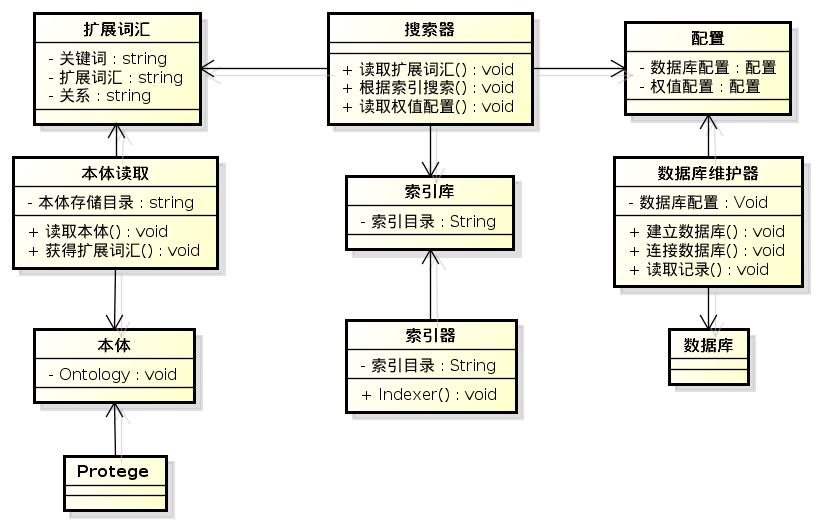
\includegraphics[width=4in]{fig/moduleInterface.png} 
	\caption{模块与接口设计图}\label{fig:模块与接口设计图}
	\end{figure}
	
	\subsection{详细设计}	
	根据概要设计中的需求,搜索核心部分被分为五个包,它们彼此的关系如图\ref{fig:包图}。
	\begin{figure}[htbp] 
	\centering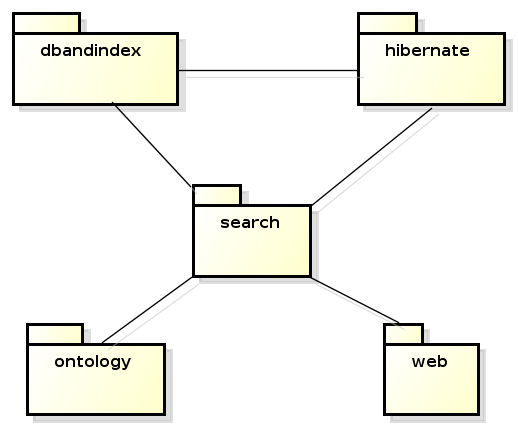
\includegraphics[width=3in]{fig/Package.png} 
	\caption{包图}\label{fig:包图}
	\end{figure}
	
	\begin{itemize}
	\item search
	核心搜索包,主要负责调用各功能模块,实现系统功能。
	\item dbandindex
	数据库和索引包,同步地将文本文件建立索引,并添加到数据库条目中。
	\item hibernate
	hibernate包,主要完成系统采用Hibernate的方式操作数据的功能。
	\item ontology
	本体包,主要完成对本体的读取和扩展词汇的存储。
	\item web
	网页包,提供高亮显示等网页预处理功能。	
	\end{itemize}
	
	下面对它们逐一进行介绍。
	
	\begin{enumerate}
	\item 核心搜索包
	
	\begin{figure}[htbp] 
	\centering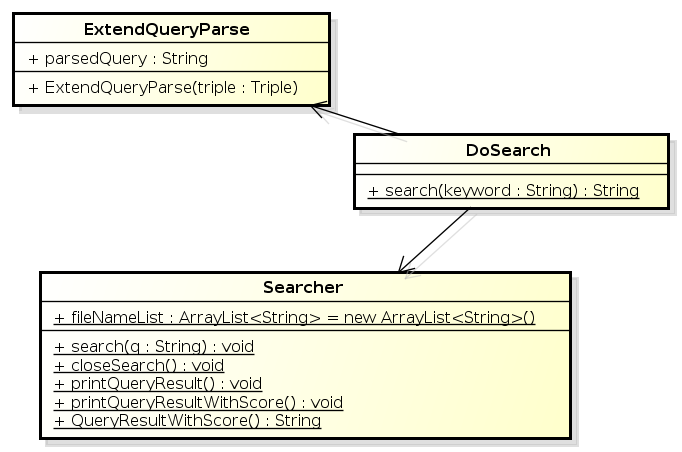
\includegraphics[width=3in]{fig/SearchPackage.png} 
	\caption{搜索包}\label{fig:搜索包}
	\end{figure}
	
	如图\ref{fig:搜索包},该包中主要有三个类:
	
	DoSearch类是后台搜索测试的入口类,由它来完成最顶级的调用;Searcher类是搜索的核心类,由它访问索引文件并完成搜索并返回结果;ExtendQueryParse类可以根据中心词汇,获得Triple类型的扩展词汇及关系表,解析成Lucene可以识别的查询语句。其工作流程大致是:首先导入本体文件,根据查询词条获得扩展词汇及关系,将其解析为Lucene查询语句,最后进行搜索。
	
	\item 数据库和索引包
	
	如图\ref{fig:数据库和索引包},该包大致分为MakeDBandIndex等几个类:
	\begin{figure}[htbp] 
	\centering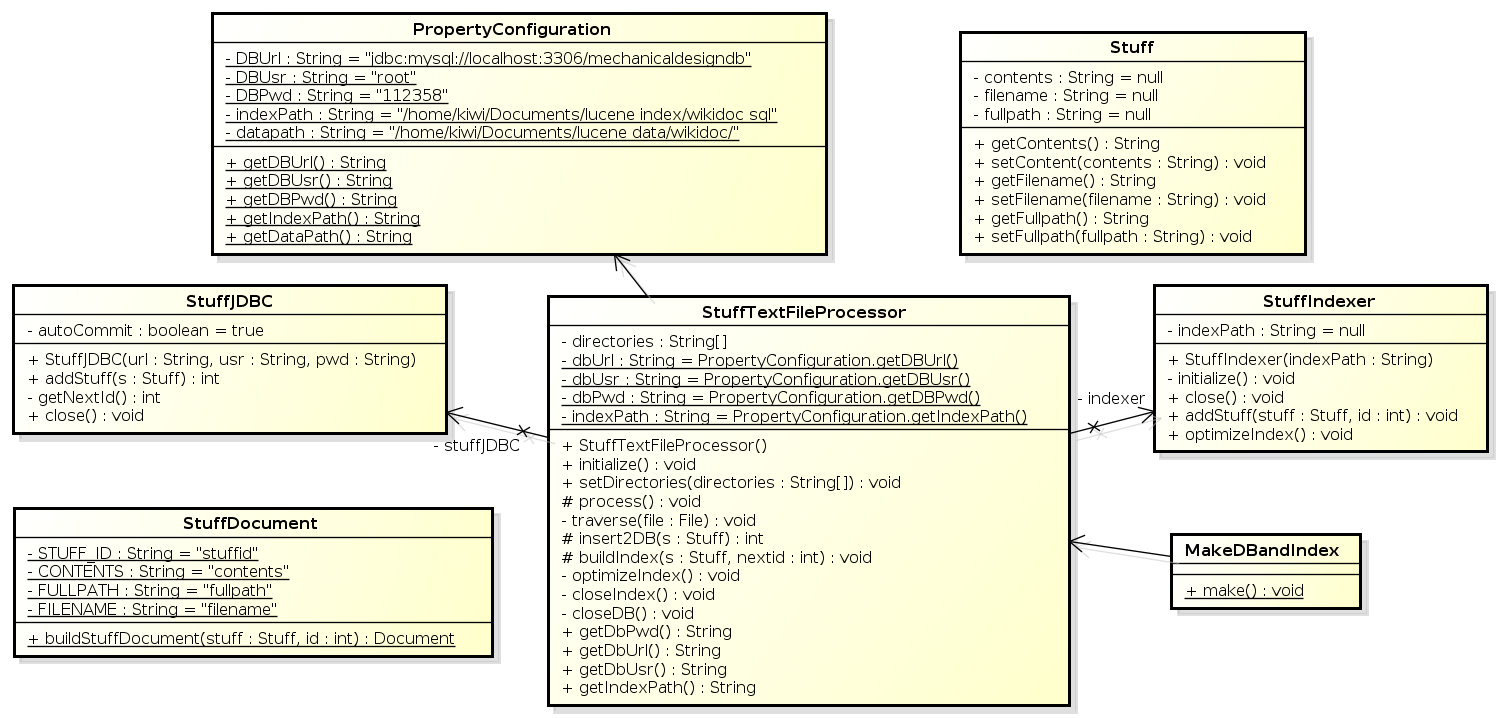
\includegraphics[width=5in]{fig/dbandindexpackage.png} 
	\caption{数据库和索引包中的类关系}\label{fig:数据库和索引包}
	\end{figure}
	
	MakeDBandIndex类是建立索引和把文本添加进数据库的总入口;StuffTextFileProcessor类是完成索引操作和数据库操作的核心类,由PropertyConfiguration类为它提供相关的参数配置;然后,通过StuffJDBC类实现与数据库的通信,通过StuffIndexer类来建立索引;接下来用traverse()方法遍历目标目录的每个文件,通过StuffDocument类对每个文本的ID、文件件、路径、内容等域进行索引操作,并把相应文件名和路径封装成Stuff类,再把Stuff类对象添加到数据库中。从而实现了索引器和数据库维护的部分操作。
	
	\item hibernate包
	
	\begin{figure}[htbp] 
	\centering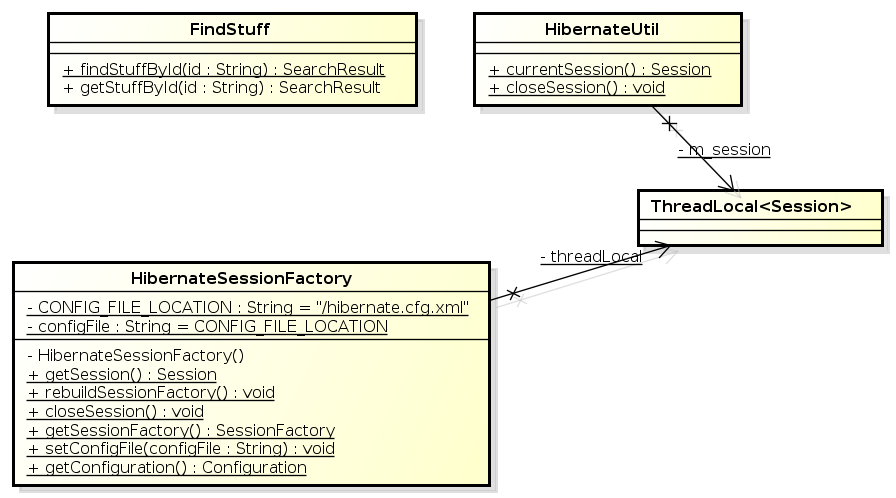
\includegraphics[width=3in]{fig/hibernatepackage.png} 
	\caption{hibernate包中的类}\label{fig:hibernate包}
	\end{figure}

	如图\ref{fig:hibernate包},HibernateUtil类、HibernateSessionFactory类是Hibernate的配置类,通过FindStuff类可以实现通过ID号读取数据库中相关记录的功能。
	
	\item 本体包
	
	\begin{figure}[htbp] 
	\centering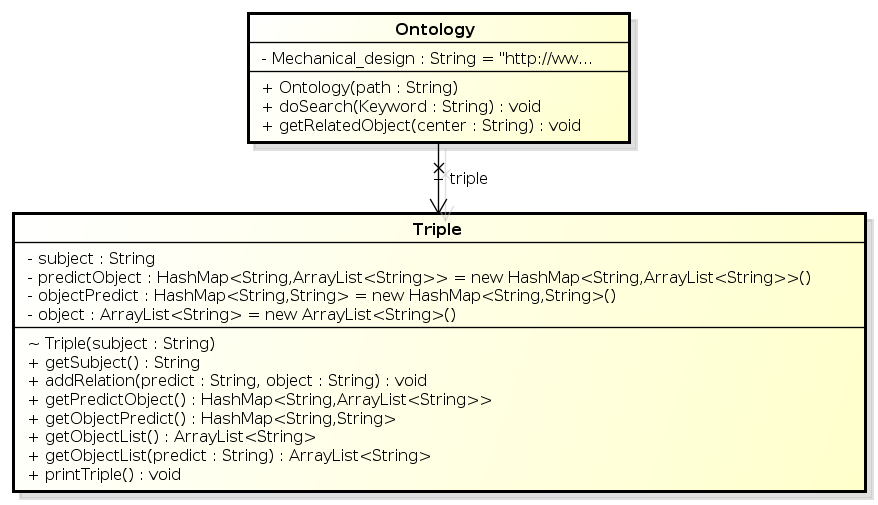
\includegraphics[width=3.5in]{fig/OntologyPackage.png} 
	\caption{本体包中的类}\label{fig:ontology包}
	\end{figure}

	
	如图\ref{fig:ontology包},本体包主要包含两个类:Ontology类能过Jena实现了对本体的读取,用它可以获得关键词在本体图中的位置,并获得了扩展词汇及它们的关系,并存储成Triple类对象;Triple类提供了一些读取中心词、扩展词、关系的方法,是实现扩展性语言搜索算法的核心。
	
	\item 网页包
	
	\begin{figure}[htbp] 
	\centering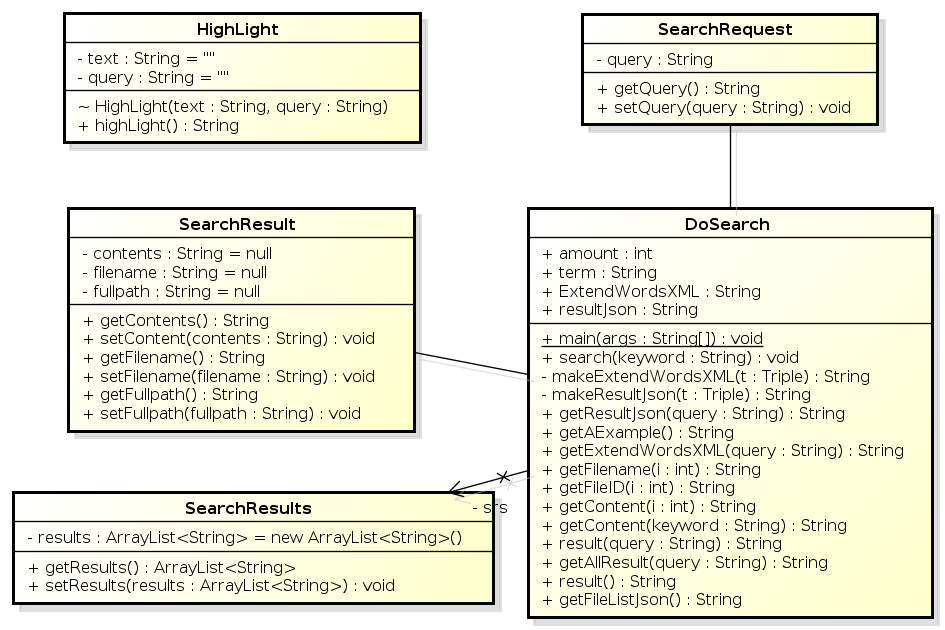
\includegraphics[width=3.5in]{fig/webpackage.png} 
	\caption{网页包中的类}\label{fig:web包}
	\end{figure}
	如图\ref{fig:web包},网页包中提供了一个给HTML文本添加高亮显示的工具HighLight类,DoSearch提供了网页访问Java类的总接口,此处更多的运用了JavaBean的思想,将搜索请求封装成DoSearch类,将搜索结果都进行封装SearchResults类,这样做有利于与前端的显示更有效地分离开来。
	\end{enumerate}

	
	\subsection{测试}
	本文通过爬虫程序从维基百科上获得了4049份机械领域的相关文档,以它作为模拟的企业内部语料库。试想对于一个设计人员而言,他需要获得关于“Gear”的相关文档,他不得不从复杂的文件夹结构中去查找,而且还只能看到文档的名字,而这个文档名字大部分时候是不能完整地表示文档的内容的。如果发现文档名相关,设计人员还需要用较长的时间去检验这些文本是否满足其查询要求。经历了那么复杂的一个检索流程,设计人员的设计思路很可能就被打断了。

	如果使用本系统,只需打开网页,以“Gear”为关键词进行搜索,就可以获得如图\ref{fig:Gear的搜索结果}搜索结果。它包含了与Gear相关的概念,这样可以启发设计人员的设计思路;相应的搜索结果,通过含有高亮显示的摘要信息,设计人员可以迅速地判断出文档的相关性,并可以在网页中直接看到文档全文。

	
	\begin{figure}[htbp]
	\centering
	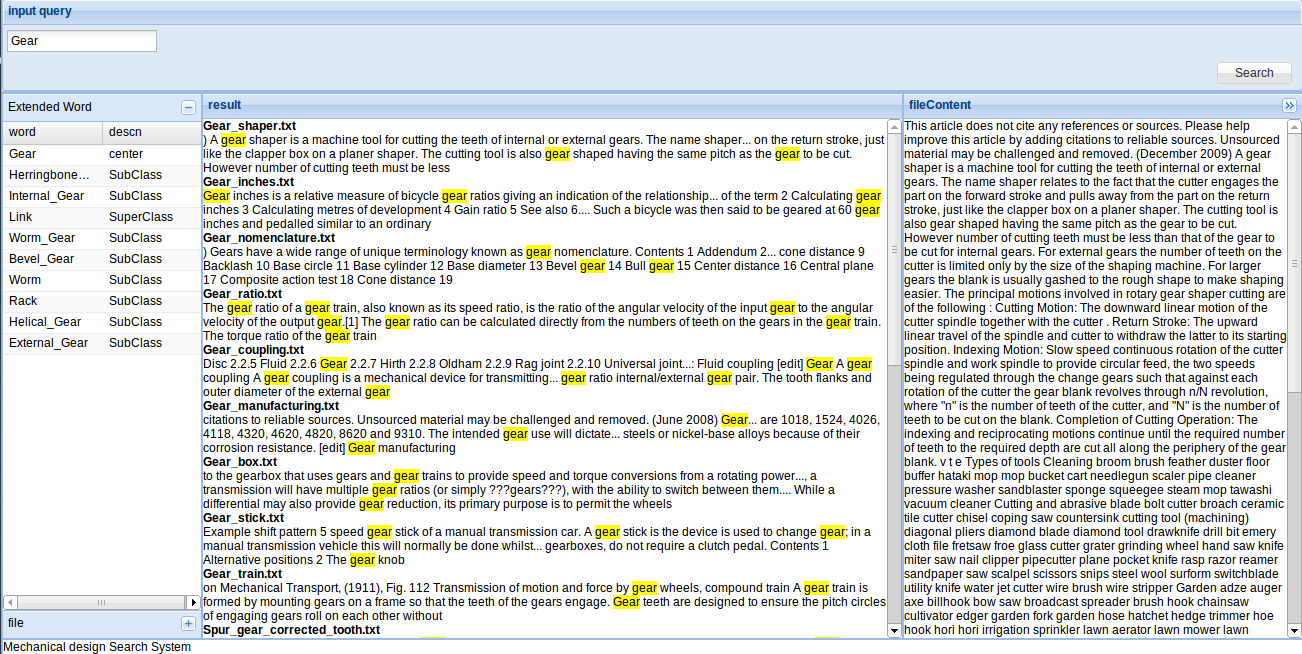
\includegraphics[width=6in]{fig/SearchResult.png}
	\caption{Gear的搜索结果}
	\label{fig:Gear的搜索结果}
	\end{figure}
	
	下面对搜索结果进行定量的分析。经过人工筛选,确定与“Gear”相关的文档有45份,分别用基于关键词搜索和用本系统的扩展性语义搜索来进行搜索。按照前文所述的绘制P-R图的方法,得出如图\ref{fig:基于关键词搜索的P-R图}及图\ref{fig:扩展性语义搜索P-R图}。

	从图中容易看出基于Lucene的关键词搜索和扩展性语义都可以保证较高的查准率,但在查全率上都显不足,只有40%,扩展性语义搜索稍稍领先。
	
	\newpage
		
	\begin{figure}[htbp]
	\begin{minipage}[t]{0.5\linewidth}
	\centering
	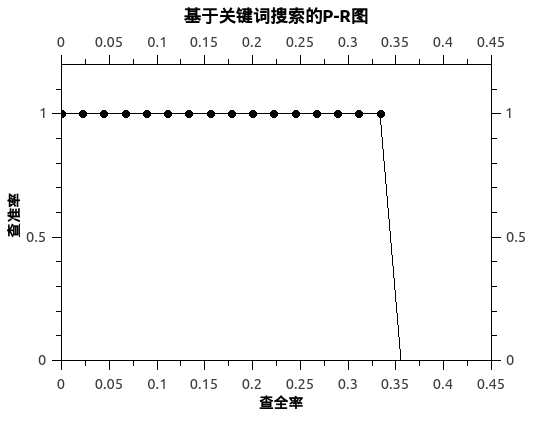
\includegraphics[width=3in]{fig/KeywordBasedPR.jpg}
	\caption{基于关键词搜索的P-R图}
	\label{fig:基于关键词搜索的P-R图}
	\end{minipage}
	\begin{minipage}[t]{0.5\linewidth}
	\centering
	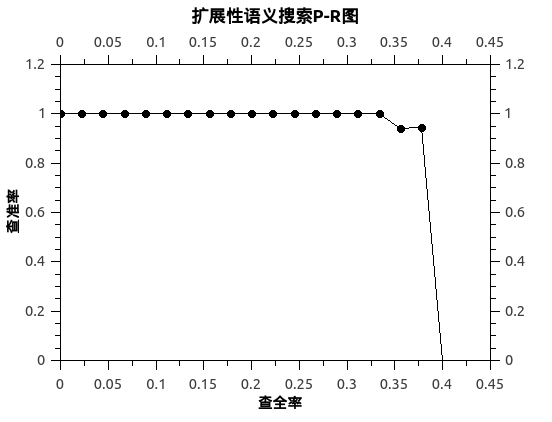
\includegraphics[width=3in]{fig/OntologyBasedPR.jpg}
	\caption{扩展性语义搜索P-R图}
	\label{fig:扩展性语义搜索P-R图}
	\end{minipage}
	\end{figure}

	

\clearpage

\section{结论}

\setcounter{figure}{0}
\setcounter{table}{0}
\setcounter{equation}{0}
	\subsection{总结}
	随着企业信息化的日益深入,尤其是对于机械领域行业,产品的全生命周期意味着企业内部文档数据的爆炸性增长,对于设计人员,要能从这些海量的文档中迅速获取他们所想要的资料,不仅能够大幅缩短设计时间,同时由于在设计阶段就已经轻松搜索获得了工艺、销售、售后的知识,从而在设计阶段就能够着眼于产品的全生命周期,既缩短了研发时间,又使产品更能够适应市场的变化。本文针对这样的需求,对机械领域知识的搜索进行了一下研究与尝试:
\begin{enumerate}
	\item 本体建模:本文讨论知识的表达形式,根据搜索的需求,确定本体表达知识的方式。研究了本体的建模方法,包括建模软件Prot{\'e}g{\'e}的使用,本体描述语言OWL,和其他的一些本体理论。
	\item 扩展性语义搜索算法:基于本体进行语义扩展,通过参数接口,可以方便地调整搜索算法的性能。显示扩展语义,能够有效地拓展设计人员的设计思路,激发创新思维。
	\item 机械领域知识搜索系统:学习了Jena、Lucene、Hibernate、JDBC等多个Java工具包,用Java编写业务逻辑,采用B/S架构,搭建本地服务器,用ExtJS编写用户前端,实现了较为完整的搜索系统。
	\item 编写相关工具集:编写了数据库维护器、索引器等附属工具,能够完成对数据库的增、删、改操作,这些通用性的工具,为今后的工作提供了支持。
\end{enumerate}
	\subsection{展望}
	囿于精力和时间,论文对机械领域知识检索系统开发还存在一些问题,需要进一步的改进和完善,在将来的工作中进行进一步的研究:
\begin{enumerate}
	\item 对中文的识别:因为英文在分词技术上具有先天的优势,能够一定程度的简化系统,所以本系统的本体构建,模拟语料库都是英文表达的,这就导致了搜索仅限制在英文为关键词来搜索英文的资料。事实上Lucene也提供了相应的中文分词包,但在前期的实验中,发现效果不理想,而做分词处理也不是本论文的重点内容,所以就避开这一问题。在今后的工作中,中文搜索是必要的,需要研究相关的分词技术,进而实现至少中英双语的搜索。
	\item 搜索内容不丰富:由于现在建立的本体规模有限,只是停留在了零部件的名称及简单的功能,并不能完全覆盖机械领域的知识,所以检索的范围就不够大。采用维基的网页作为模拟语料库,从数量和类型上,都与企业内部的技术文档有一定差异,搜索结果的优劣并不能单纯以一个PR图来判断,需要通过用户的使用、反馈才能得到合理评价。
	\item 搜索速度较慢:本论文只着眼在了系统的功能实现,对于效率问题考虑还不够多,搜索过程在秒级,与专业的搜索引擎毫秒级的搜索速度还有着较大的距离。
\end{enumerate}
\newpage	
\renewcommand\listfigurename{图片索引}
\renewcommand\listtablename{表格索引}
\addcontentsline{toc}{section}{图片索引}
\listoffigures

\newpage	
\addcontentsline{toc}{section}{表格索引}
\listoftables

\newpage

\addcontentsline{toc}{section}{参考文献}%在目录中添加“参考文献”的标记
\wuhao %五号
\setlength{\baselineskip}{17pt} %设置行间距17pt
\renewcommand\refname{参考文献}\

\bibliographystyle{unsrt}  %按引用顺序排列
\bibliography{reference.bib}	

\newpage
\section*{致\quad 谢}
\addcontentsline{toc}{section}{致谢}


\setlength{\baselineskip}{20pt} %设置行间距20pt
首先,谨向我的导师田凌教授致以最诚挚的谢意。田凌老师较早地将我安排进入实验室,鼓励我参加学校和实验室内部的各类学术活动,让我较早地找到自己的角色。毕业设计期间,在学习、研究、生活上给了我无微不致地关怀,耐心解答在学术层面和思想层面的各类为题。本论文的选题、研究和写作都得到了田老师的耐心的指导。田老师严谨的治学态度、开阔的学术视野、诲人不倦的高尚师德让作者如沐春风,受益匪浅。

然后,要感谢实验室的马嵩华师姐、武园浩师兄、段文睿师兄、刘钡钡师兄、王占松师兄、李春光师姐等师兄、师姐。马嵩华师姐在课题的细化,切口的选择,研究思路的确定等多方面都给予了极大的帮助;武园浩师兄在课题前期为我提供了相当多的技术指导与支持,对于毕业设计项目也多次提出宝贵意见;其他师兄、师姐也在各个方面为我提供了极大的指导与帮助。

最后,感谢我的班主任、我的同学、我的父母一直以来对我的支持与鼓励。

\newpage

\addcontentsline{toc}{section}{附录 A 外文资料的调研阅读报告或书面翻译}
\section*{附录 A 外文资料的调研阅读报告或书面翻译}
 
\begin{center}
An ontology-based retrieval system using semantic indexing

基于本体的语义检索系统
\end{center}
\renewcommand{\thetable}{\arabic{table}}
\renewcommand{\thefigure}{\arabic{figure}}
\setcounter{figure}{0}
\setcounter{table}{0}
\xiaosihao
\setlength\parindent{2em}
\setlength{\baselineskip}{20pt} %设置行间距17pt
\renewcommand\refname{参考文献}

摘要

在这篇文章里,我们展现了一种基于本体的信息抽取和检索系统,以及它在足球领域的运用。总的来说,我们解决了在语义搜索中的三个问题,也就是,使用性,可扩展性和检索效果。我们提出了一种基于关键词的语义检索方法。使用具体领域的信息抽取之后,系统性能得到了显著的提升。通过语义索引方法以及用一个小的独立模型来代表世界,可扩展性也得到了实现。系统用全世界最先进语义网技术来实施,其性能可与传统方法和扩展查找法相媲美。此外,我们还提出了一种具体的评价指标,来观测专门领域的信息抽取与推理的性能表现。最后,我们展示了我们是如何采用语义检索的方法来解决简单的结构性二义性的。

1.导言

互联网上可获得信息的数量与复杂性都在爆炸性增长,人们就迫切需要一种工具和技术来通过语义地掌握这些数据。现在的信息检索方法主要基于搜索全文的关键字,也就是一个海量词包的模型。然后,这样的模型丢失了很多真正的文本语义信息。为了解决这个问题,本体技术,作为一种知识表达的方式就应运而生,它也成为了当今语义网应用的支柱。能够给普通文本赋予语义的元数据,也就为信息抽取和检索过程提供了极大的便利。

当语义知识通过本体表达出来,下一步就是要查询语义数据,也就是语义搜索。现在有几种用于语义查询的查询语言。现在,{\Times SPARQL}是语义网最先进的查询语言。但不巧的是,这些正式的查询语言并不能很好地被末端用户使用。用这些语言严谨描述一个查询需要领域本体和语言的语法。因此,语义网研究团体为末端用户简化检索过程。当下的语义检索接口研究主要包含了四种类型:基于关键词的,基于形式的,基于视觉的,基于自然语言的。其中,基于关键词是操作最友好的,人们也习惯于使用这种接口,在这个问题上,幸亏有谷歌搜索。

在语义搜索领域,能够整合关键词方法的易用性和语义技术的强大性,是极具挑战性的技术。根据我们对语义网的观察,所有对保证用户友好层的基础上提高检索性能的努力都会带来这样的结果,那就是改善采用关键词接口的语义搜索。这是一项极具挑战性的任务,因为它需要用简单的关键词完成复杂的检索。此外,它还要求能够使推理信息得以被轻易检索,并且提供一种排序机制反映语义和本体的重要性。

在本文中,我们展示了一种完全基于本体的框架来实现对特定领域的语义信息的抽取和检索。这个系统含有爬虫模块,自动的信息提取模块,本体运用模块,推理模块,和关键词语义搜索的界面。我们主要考虑的是创造一种可扩展的、用户友谊好的、检索性能优异的检索系统。我们把这个框架运用在了足球领域,并且看到了相对于传统的关键词搜索的显著提高。我们展示了我们系统对于足球领域非常复杂的查询也实现了极高的查准率和查全率。此外,我们评估并报告了依照语义性过程(只采用信息抽取和同时采用信息抽取和推理)在不同程度的索引方法下的查询效果。

可扩展性被分为两个主要方面来考虑:推理和查询。在推理方面,可扩展性要求把完全的逻辑模型拆分成单独的独立模型,因为在一个大模型下搜索比在一堆小模型下搜索要复杂很多。一些相似的研究也着眼于用一个模型来描述整个世界。因此,他们并不能匹配大尺度的。

在查询方面,可扩展性要靠把推理的知识转化成一个单独的逆索引结构来保证。用这种逆索引结构可以把我们的系统向上扩展到网页搜索引擎,也就意味着可以在较短时间内完成几百万个搜索,并且从少量的数据中检索出想要的信息。它也触发了关键词搜索的使用。用这种方法,就可以支持用户友好的查询方式。基于信息检索的本体研究采用本体模型中的逻辑查询。因此,相比于网络尺度来说,它只能被用在较少量的数据搜索中,而且对于普通用户来说,逻辑搜索也是一个困难的工作。

文章的剩余部分按照如下思路组织:在第二部分简要讨论相关的研究工作成果,在第三部分系统的主要组成部分,也就是信息抽取,本体构建、推理和信息检索。在第四部分,我们给出了评估结果。第五部分给出与扩展搜索方法的简单比较。第六部分阐释了系统支持短语描述扩展的机理。第七部分,我们进行简单的讨论,在第八部分,总结全文,并对未来工作进行展望。

2.相关研究

经典的,或者说传统的基于关键词的信息检索方法是基于{\Times Salton}等人提出的向量空间模型。在这种模型中,文本和查询都是被简单的表述关键词术语权值向量,检索就根据这些向量的余弦相似度来完成。与传统搜索相关的重要工作在文献4~7中描述。这种方法不需要任何抽取或者是注释语句,因此它更容易实施,然而,查准率相对较低。向量空间在现实生活中的运用,是采用了诸如{\Times Lucene}的逆索引结构来实现的。换句话说,{\Times Lucene}类似的工具建立了向量空间模型的理论背景和现实世界应用的联系。

语义检索的第一部是要利用词汇网络的同义词表解决单词语义。其主要思想是利用单词的主义来同时扩展目录和查询,以期更好的查准率和查全率。如果同时采用了有效的词感模糊算法({\Times WSD}),这种方法提升了检索性能。从另一方面说,一个不好的WSD将会导致性能下降。这种方法的另一个缺点是缺乏复杂主义,因为他被局限在了词汇网络的有限关系中。

语义检索的下一步是采用信息抽取。有很多这个领域的研究。他们主要的区别在于资源的结构,抽取信息的细节和计算/记忆资源。基于{\Times NLP}的方法是独立的,因为使用了句子的解析树,自动词性赋码器,数据块解析,首语重复解决方法等,以期能够抽取信息。他们都需要大量的计算过程。也有一些信息抽取方法的选择,比如基于特征/规则的信息抽取就不用特别庞大的计算开销。这些方法根据特征/规则的创建形式来分类:自动,手动。如果考虑在某一个领域付出的劳动的话,相比于手动法,自动法显得更高级,但其查准率查全率又不理想。

文献22~26使用的方法是采用人工建立的规则来抽取信息。人工建立规则也被用于语义性的注释。{\Times Etztioni}等人用独立的规则来定位文本中不同类型的个体。{\Times Wessman}等人主要依靠常规表述。{\Times Cerno}是一个用于领域本体描述语义性注释和文本文档的轻量级框架。它整合了基于关键词和基于结构的注释规则,而不是语言学的特征。我们需要一种可扩展的,应对刚性结构化领域的信息抽取方法。这种方法应该也能被用于土耳其语和英语内容。由于抽取信息的细节对我们的目标非常关键,我们必须非常关注查全率和查准率直。因此我们采用了手动填加的方法,因为在其中,技术细节已经被给出了。

关于本体设计、集成和重组的研究提供了很多基于本体的信息抽取和检索方法。{\Times Oberle}等人提出了一种基本的本体,{\Times SmartSUMO},它是基于{\Times DOLCE}和 {\Times SUMO} 本体的,其目的是集成用于智能网络的领域本体,最后的集成本体被称为智能网络集成本体({\Times SWIntO})。因为 {\Times SmartSUMO}同时具有语言学特性,{\Times SWIntO}被用在基于本体的文本信息抽取。也一种面向本体设计的固定方法。文本信息用一种健全的方法被映射成为本体概念。然而,整个集成本体在遇到一个新的语言结构就会受到影响,因为语言性特征就是基础本体的一部分。为了避免这种困难,词汇特性要被独立于基础本体和领域本体来考虑。我们选择的本体设计并不考虑基础本体,因为我们暂时还没有针对不同领域的集成目标。然而,我们通过一种把词汇特性映射到本体的信息抽取方法,保留了词汇信息独立于本体的思路。就基于本体的信息检索系统的各个方面问题,现在都进行了很多讨论。文献34的基于本体的信息检索研究,主要着眼于让{\Times MPEG7/21}标准与领域和应用本体之间能够彼此协作。在我们的研究中,我们开发了一个中心足球本体,它可以表现出足球领域的知识。我们的本体被认为与文献34中的足球本体在独立于互用性的领域知识方面一样强大。另一方面,文献34中提出的检索方法是严格的。因为检索方法都是基于逻辑查询的,建立搜索查询对于一般的用户来说是极困难的。在这个条件下,我们提出了一种基于查询结果方法的索引,使用户可以用一种简单灵活的方法来查询基于本体的知识。

文献35讨论了本体用于在组织记忆中进行信息检索,探究了组织化,访问性,保存大量异相信息的元级描述的重要性。也有研究提了了有理解力的元级模型和检索的基于本体的方法。本体可以分为几类:领域本体,信息本体,企业本体等。他们都采用一种常规的面向对象的形式进行建模。根据这个分类,我们用领域本体来代表足球比赛,这个领域本体被用于推理那些从比赛总结中没有精确提取的信息。在我们的研究中,没有明确的搜索。我们都用逆索引来重构推断的信息,并提供查询结果。

在一个信息检索系统中,用于查询本体知识的用户界面是至关重要的一个点。通用的方法是把解析出的数据以{\Times RDF}或{\Times OWL}的形式存储起来,再用{\Times RDQL}或 {\Times SPARQL}等查询语言云查询{\Times RDF}。尽管这种方法有极好的查准率和查全率,它还是不能用于实用,因为它需要相对复杂的查询语言。为了克服学习一种正式查询语言的困难,现在又提出了很多查询页面的方法。正如我们早些所说,我们主要的重要应该放在的有几种方法在基于关键词的界面。目前有几种方法是实施了基于关键词的搜索的。简单地说一说,{\Times SPARK}用了概率查询排序法来找出关键词所代表的最佳查询。{\Times Q2}语义尽力在一个{\Times RDF}图中找到代表查询的最佳子图。{\Times SemSearch}用了一种基于模板的方法来进行查询。这些方法都不容易被扩大到大量知识的情况,因为他们都需要{\Times RDF}图或是为了一次搜索要对同样的基础知识进行多次查询。

一种可扩展的从关键词进行查询构建的选择是语义索引。在这种方法中,{\Times RDF} 基础知识中的语义数据被用一种结构化的方法索引,并且能直接为关键词查询所用。一种相似的方法被用在了文献40~42中。他们为所以{\Times RDF}中解析出来的三元组和相关的自由文本做了索引。因为他们采用了非常基础的的提取方法,这样一种简单的索引看起来是可行的。然而,从只包含了主谓宾的索引中并不能提取出复杂语义。如果要求系统能够从解析和推理的知识中完成复杂查询,那么索引就必须被进行相应的设计和充实。在文献43中,展示了一种基于多模式通用语义网搜索接口,以及其在2006足球世界杯中数据的运用。重点在于形成一种回答问题的系统,它能够考虑到基于与用户交互的论述和上下文的信息,并且以语义网为基础形成一个语义查询。据记录,对于某些查询,这个过程的次数上升到最小2次。考虑到查询与文献43所提到的足球相关,我们的系统不仅成功地控制了所有的数据,而且通过利用语义索引实现了即时查询,强调了可扩展性和性能表现等问题。此外,我们的本体个体是通过网络描述的信息自动抽取出来进行构建的,然后再基于推理应用规则使其充实。

我们的文献调研提示了当前基于关键词语义搜索的研究是不够成熟的:他们即不能扩展到大尺度的基础知识,也不能在查询中捕获所有的语义。我们的主要贡献是通过实施一种基于关键词的使用语义索引方法的语义检索系统,填补了这方面的空白。换句话说,我们尽量的实施这样一种系统,其表现至少与传统方法一样好,能够在性能和语义查询的实用性上有所提高。我们在足球领域检测我们的系统,看看传统搜索方式之上的语义搜索的有效性,我们观测到了查准率和查全率上可喜的提高。我们注意到我们的系统可以完成复杂语义的查询,而传统方法是不可能做到的。本文所展示的方法可以通过修改现行的本体和文献30所述的信息提取方式,被扩展到其他领域。

3.我们语义检索的方法

在本文范围内,我们开发了一种完全成熟的语义应用,它包含了从信息提取到信息检索的语义网的各个方面,并且使用了所有的分词技术,比如{\Times OWL-DL},推理,规则,{\Times RDF}库和语义索引。框架的全部图解如图一所示。后面的部分以对全对程的简单总结开始,描述了系统的几个重要方面。

	\begin{figure}[htbp] 
	\centering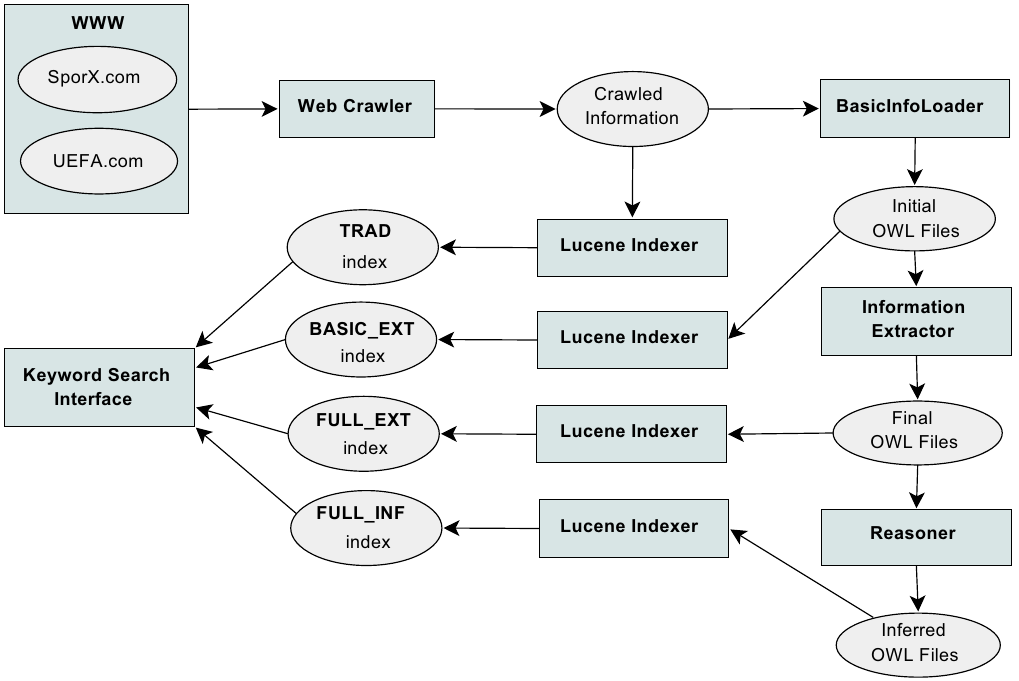
\includegraphics[width=5in]{fig/trans/fig1.png} 
	\caption[]{\xiaosihao 系统框架图}
	\end{figure} 
3.1全过程

在给出各模块的技术细节之前,我们认为先来看看我们用于足球领域的系统的全工作流会很有帮助。接下来,我们描述在系统准备好进行语义查询和评估之前的步骤。

{\Times a}.通过爬虫在{\Times UEFA}和{\Times SporX}等网站上获得有用信息,并临时性地存储起来。所得数据包括了一些基本信息,比如队伍、队员、进球、替补、每场球赛的场馆,以及以自由文本形式工出现的按时间的解说。

{\Times b}.只用自由文本的解说来建立索引,{\Times TRAD},以进行传统的关键词搜索。

{\Times c}.用这些基本信息和解说,我们建立了原始的{\Times OWL}文件。

{\Times d}.通过这些原始{\Times OWL}文件,我们建立第二个索引,{\Times BASIC\_EXT},它包含了基本信息和解说。这个索引只是为了评估而建立(也就是说,用它和索引{\Times FULL\_EXT} 进行比较,后者是在信息抽取之后建立的)。 

{\Times e}.上一步建立的{\Times OWL}文件通过信息抽取模块读取。这个模块建立了具有从解说中提取出来的信息的{\Times OWL}文件,信息包括越位,犯规,角球等,以此来获得最终的{\Times OWL}文件。

{\Times f}.读取并索引这些{\Times OWL}文件,从而建立{\Times FULL\_EXT}。

{\Times g}.我们对这些文件运行了推理机,获得了一个新的包含推理信息的新的{\Times OWL}文件

{\Times i}.最后,我们用这些推理的{\Times OWL}文件建立一个索引,{\Times FULL\_INF},也就是最后一个用于语义搜索的索引。

尽管我们在研究中只着眼于足球领域,但是上述方法可被运用到其他有给出本体的领域。这个系统最针对某个领域的模块是{\Times IE}模块,它应该被扩展来解决其他领域的问题。文章的剩下部分描述了系统的几个主要组件。我们以建立领域本体开始,然后是{\Times IE}和{\Times IR}组件,最后我们来看看评估结果。

3.2本体设计

本体是概念和概念之间关系的一种描述。他们通过提供真实世界对角的共用知识,在语义网络应用中扮演重要角色,它也有效提升了重用性和不同模块之间的互换性。因此,本体的质量是任何语义应用的首要考虑的问题。

对于这项研究,我们设计了一个中心足球本体,它利用了这个系统的各个方面,尤其是在信息抽取,推理和检索词组等方面。在本体设计阶段,我们遵循了一个迭代的过程。首先,我们以一个包含核心基本概念和一些简单分类的本体为起点。然后,我们用这个本体进行实验,解决了其在推理和搜索中的一些问题。这些步骤一直重复,直到我们得到了一个含有79个概念和95个属性的足球领域的稳定本体。完成的类树如图2所示。

	\begin{figure}[htbp] 
	\centering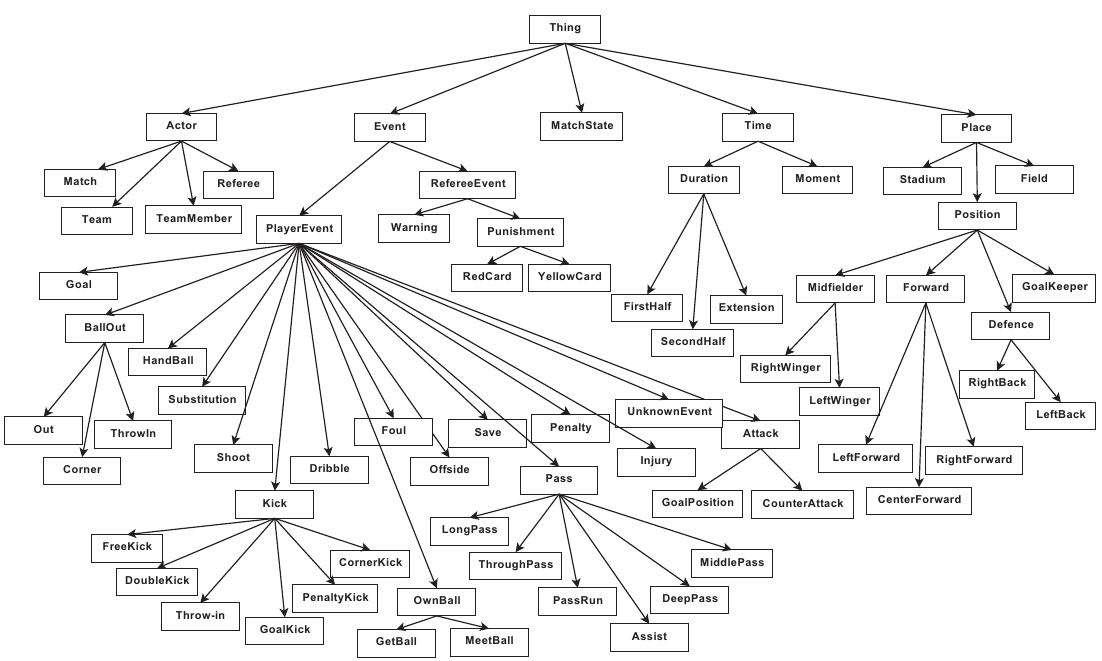
\includegraphics[width=5in]{fig/trans/fig2.png} 
	\caption[]{\xiaosihao 领域本体,类结构}
	\end{figure} 

3.3 信息抽取({\Times IE})

信息抽取是基于本体的语义网应用的重要组成部分。它是把非结构化的资源转化成结构化的信息,并存入信息基础的过程。在这个阶段,我们用爬虫从{\Times UEFA}和{\Times SporX}获得的数据。我们所获得的东西是一些具体到比赛(队伍,队员,进球,场馆等)的信息和一些自然文体(关于比赛的不断的解说)。这些基本信息和解说被用作信息抽取模块的输入。这个模块的技术细节在文献30中有描述。在研究中,我们只是从功能角度进行了概览。

基本上,这是一个基于模版针对具体领域的{\Times IE}方法。不像其他自动方法,它并不采用词性标签,语法剖析器和短语识别等语言性的工具。因此我们的方法可以被用在任何领域,任何语言,而不必彩语言工具,尽管人工建立模板是它的一大缺点。{\Times IE}模块的细节可以总结成了两个部分:命名实体识别器和词汇分析器。

3.3.1 命名实体识别器({\Times NER})

如之前所提到的那样,{\Times IE}模块把一些诸如队伍、队员的信息作为输入作为解说的补充。这些信息被用来识别和分类解说中的命名实体。通过运行{\Times NER},队伍名称和队员名称被{\Times <team1>},{\Times <team2>},{\Times <team1player5>}这样的标签所取代。例如,一个句子“{\Times Iniesta}得分”就可能变成“{\Times <team2player11>}得分”,如果{\Times Iniesta}是这只队伍的11号的话。

3.3.2 两个层次的词汇分析

这是我们{\Times IE}模块最关键的部分,在这儿,复杂的语义实体和关系都将根据预先定义的模板进行解析。第一个层次是要定义关键词/词组并且忽略剩余的部分。第二个层次是把第一层的输出作为该层的输入,并且根据预告定义的模板进行解析。根据我们的调查,大多数语义网的研究都缺乏这种类型的解析,因为他们通常对NER产生的注解就很满意了。

根据文献30所述,多亏了{\Times UEFA}网站的高度结构化文本和零错误,我们得以实现{\Times UEFA}解说的100%的成功率。图3给出了我们可以从{\Times UEFA}网站抽取信息的想法。这个模块与系统的集成采用了时下流行的松散耦和形式,所以我们能够把它用于任何语言任意领域的语义性应用中。

	\begin{figure}[htbp] 
	\centering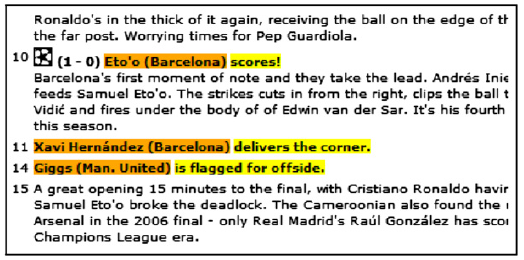
\includegraphics[width=3in]{fig/trans/fig3.png} 
	\caption[]{\xiaosihao {\Times UEFA}解说解析样例}
	\end{figure} 

3.4建立本体

建立本体的过程是要把非结构化、半结构化或结构化的数据转换或是映射成本体实例,以此获得知识。我们的信息抽取模块在把非结构化的文本解说解析成结构化的信息方面已经完成了大部分工作。例如,在解说词“{\Times Keita}在与{\Times Belletti}争抢时犯规“,我们就获得了一个犯规对像,更具体的说,就是{\Times FOUL (Keita, Belletti)}。

有了{\Times IE}模块的输出,建立本体的过程变成了为{\Times IE}所获数据的每个对象建立{\Times OWL} 实体。正是在这个阶段,{\Times IE}模块与系统的其他部分进行了集成。我们尽量让这种集成松散。通过定义高层的属性,我们解决了本体层折问题。一般情况下,本体里的每一个事件都有其一套属性。例如,根据一个事件的主语,一个犯规实例就有被罚球员这样一个属性,而一个进行实例就会有得分球员这样一个属性。问题在于通过{\Times IE}模块的信息来填补正确的属性值。我们对这个问题的解决方法是为本体中的每个事件定义四个一般属性,{\Times subjectPlayer}, {\Times objectPlayer}, {\Times subjectTeam}和 {\Times objectTeam}。这些属性都是一般的,针对每个事件还有具体的子类属性。例如进球事件就具有属性得分球员,它恰是 {\Times subjectPlayer}的一个字类属性。用这样的方法我们可以自动的通过这个事件的发出者,在得分事件中填补进球事件。相似地在受伤事件中受伤队员属性,就会被填以这个事件的客体,因为受伤队员属性在本体中被定义成了{\Times objectPlayer}的子类属性。

如果{\Times IE}模块不能解析一个事件中的任何一个属性, 我们可以创建一个有空属性的实例。因此,哪怕{\Times IE}没有能解析出事件的一些属性,对于简单查询查全率也不会受影响。此外,如果解说中没有提及事件,一个具有未知事件的实例也会被创建。未知事件并没有丢失,原因见如图4所示的起始于{\Times UEFA}解说、终止于{\Times OWL}实例的过程之描述。

	\begin{figure}[htbp] 
	\centering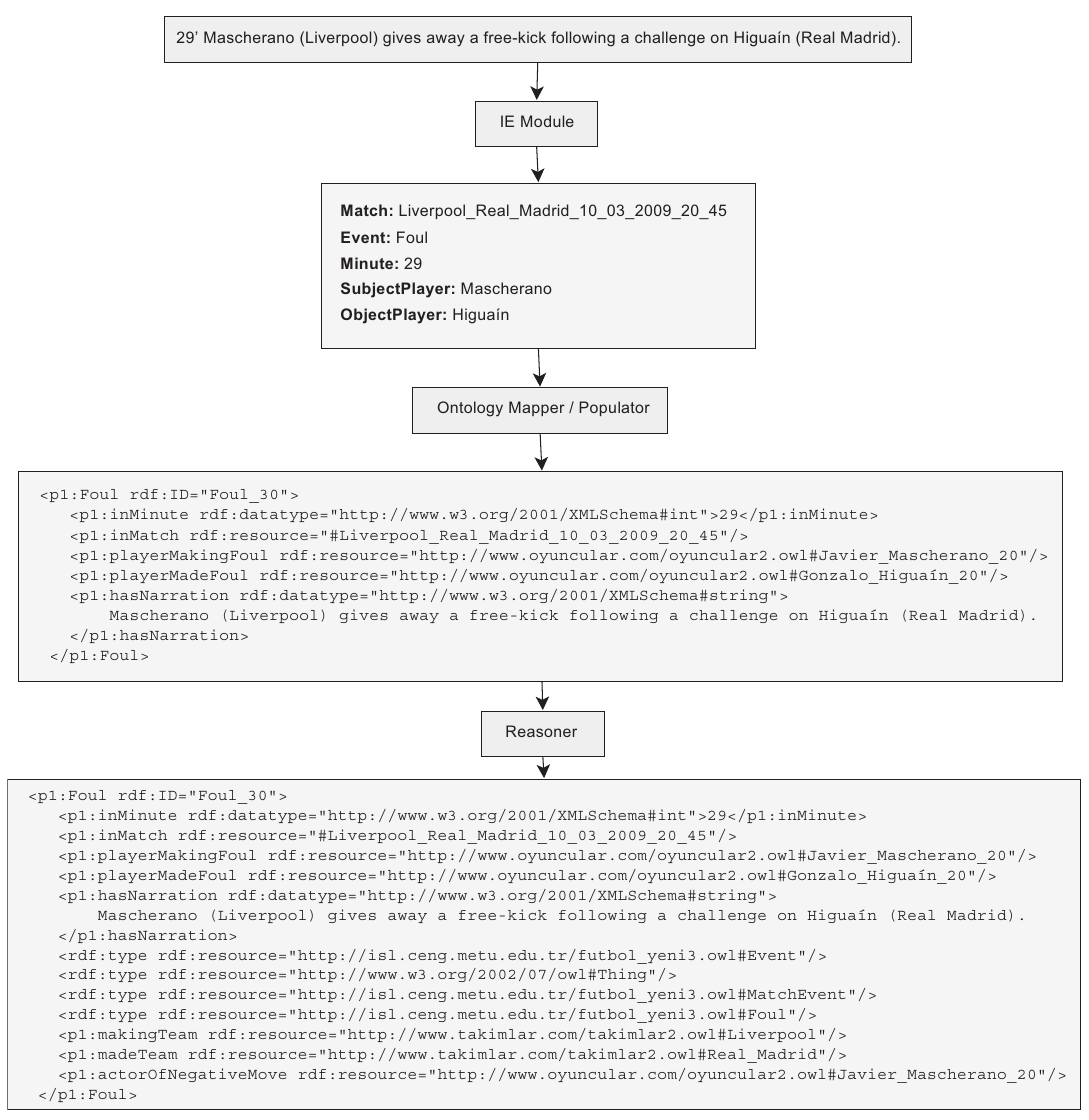
\includegraphics[width=6in]{fig/trans/fig4.png} 
	\caption[]{\xiaosihao 信息获取和本体化}
	\end{figure} 

用{\Times IE}模块解析事件进行本体建立并不严格,如之前所谘的,爬虫数据包含了关于比赛的基本基本信息,包括队员,队伍,裁判,场地等,这些信息如果在基础知识中不存在,则通过建立{\Times OWL}实体逐个填加到文本中。

3.5推理和规则

网页本体语言,{\Times OWL},是一个正式的标准,它很大程序上被描述逻辑({\Times DLs})影响着。{\Times OWL DL}是由计算机完成的,{\Times OWL}的可决定版本,它得益于有很多可靠完整{\Times DL}推理机。对于我们的推理模型,我们用了{\Times Pellet},一种开源的{\Times DL}推理机,它支持各种标准的推理服务,比如相容性检查,概念可满足性,分类,实现。

相容性检查保证了本体中没有相矛盾的声明。为了利用这种特性,我们在本体构建过程中细化了一些属性的约束条件。{\Times OWL}中有两种约束条件:值约束和集约束。我们用了值约束,比如,要陈述只有守门员(队员的子集)才被允许待在守门位置,然后用集约束,我们可以说一场比赛只允许有一个守门员。这些约束条件不仅在相容性检查中发挥作用,而且使得新信息可以被推断出来。例如,当某个实例的某个属性值的定义域被限制在一个特定的类,那我们可以推断出这个实例的类型了。

采用分类推理,我们可以根据本体中的类和子类的定义得到完整的类树。通过分类来推断新知识是独立于领域的过程,并且它对基础知识的影响是小的。如图5所示是一个简单的例子,长传的类树结构就是被推断出来的。

	\begin{figure}[htbp] 
	\centering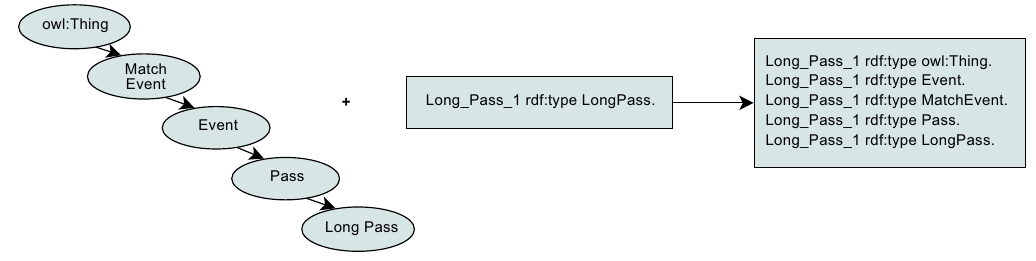
\includegraphics[width=6in]{fig/trans/fig5.png} 
	\caption[]{\xiaosihao 常传的类层次推理}
	\end{figure} 

为了推理更多的有意思的信息,我们用了{\Times Jena}规则。为了证明{\Times Jena}规则的强大之处,我们给出一个推理助功事件的例子。采用如图六所示的{\Times Jena}规则,我们能够在基础知识中增加一个助攻实例。这个规则只是找两个事件,一个是得分一个是发生在同一场球赛,同一个时间,接伟球的人恰好是得分的那个传球。如果是这种情况,那么就建立一个助攻实例,并把它填加到基础知识中去 。

	\begin{figure}[htbp] 
	\centering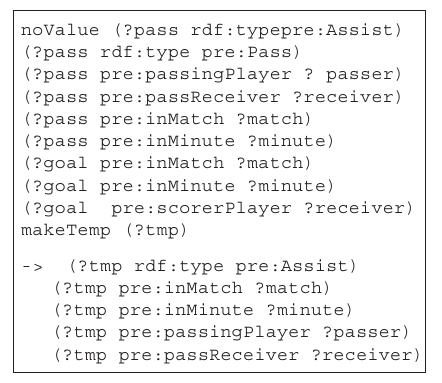
\includegraphics[width=3in]{fig/trans/fig6.png} 
	\caption[]{\xiaosihao Jena规则范例}
	\end{figure} 

推理是一个需要开销的过程,尤其当声明数量很大的时候。这个问题要被妥善地解决才能保证系统的可扩展性。因此,为了解决这个问题,我们采取了一些措施。首先,我们保证每场球赛是彼此独立的,然后单独进行推理。然后,我们分离地把推理得到的信息加入到基础知识中云。所以,推理球赛所需的时间就与球赛的数量无关。第二,所以的推理任务,包括分类和推理,都是线下完成的,也就是优先查询。这样一来,因为在运行的同时不会有线上推理,就可以提供可扩展性和查询效率。

3.6语义索引和检索

要查询一个语义性的基础知识并检索结果有很多方法。这些方法被分为四大类,基于关键词的,基于自然语言的,基于视觉的,基于形式的语义性搜索。在这些方法中,基于关键词的接口为末端用户提供了最轻松舒适的查询方法。对于其他方法,尽管他们可以实现更为精确的查询,但是需要更多的依赖于领域大小的用户交互。尽管基于关键词的接口,有着歧义等缺点,但是也存在一些方法可以缩小这一点,我们在第6部分将会有阐述。现在,已经决定了用基于关键词查询,下一个问题就是怎样才能实现好的检索性能和可扩展性。答案很简单,采用语义性索引。

正如我们之前文献调研所提到的那样,现在的关键词方法要么在大体积的{\Times RDF}文件中进行实时的遍历,要么只是用了简单的{\Times RDF}三元组关系。换句话说,他们没有同时考虑到可扩展性和检索性能。我们提出了一个叫语义索引的模型,它继承了传统关键词搜索,并用领域本体进行信息抽取和推理。这种索引机制是基于{\Times Lucene}的,这是一个可扩展的性能优异的索引器和搜索器。通过继承{\Times Lucene}索引的定制排序,含有本体信息的文本就有更高的权值,这样一来就实现了语义性检索。索引结构和排序的细节将在3.6.1和3.6.2部分分别详述。

3.6.1索引结构

语义索引的结构在检索性能上起着至关重要的作用,我们建立了一个{\Times Lucene}索引,每一个条目代表一个足球事件。正如我们在上一部分所说的那样,每一个事件都有与之相联系的属性,比如主体和客体。信息也被包含在了各个事件中。我们在索引中也包括了与事件相关的文本解说。如果一个是事件是未知事件(一个没有被信息抽取机识别的事件),这一点将非常重要。把全文解说加入到索引中,可以容忍事件信息的不完整性,因此可以保证在传统全文搜索中的查全率。索引结构及例子在表一中可见。


	\begin{table}[htbp] 
	\centering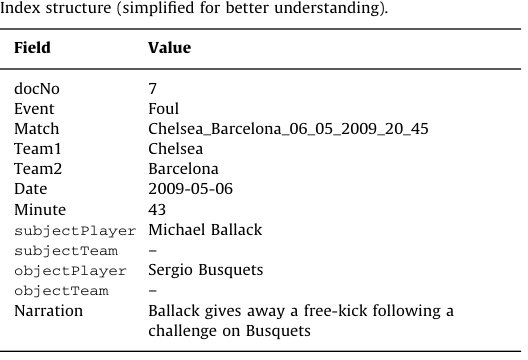
\includegraphics[width=3in]{fig/trans/tab1.png} 
	\caption[]{索引结构(为了便于理解简化)}
	\end{table} 

对于推理{\Times OWL}文件,我们建立了索引的扩展版,补充了索引中包含的基本信息,推理之后的索引也包含了事件的推理类型域,一个推理队员属性域和一个根据语义规则推理出的信息域。这些增加的信息都被加入到了推理索中,见表2 。注意主队和客队域也是用语义规则推理出来的。

	\begin{table}[htbp] 
	\centering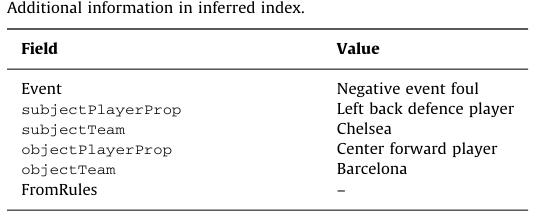
\includegraphics[width=3in]{fig/trans/tab2.png} 
	\caption[]{推理索引的补充信息}
	\end{table} 
3.6.2搜索和排序

在传统的关键词搜索中,索引文档通常除了一些与文档有关的粗糙的文本就什么有没有了。{\Times Lucene}能够轻松地控制索引,而且其默认排序就能给出很好的结果。然而,针对复杂的索引就要谨慎对待了。为了利用好我们面向索引结构的本体,我们稍微地修改了{\Times Lucene}中默认查询和排序机制。首先,我们扩大了排序域,包含了解析和推理的信息,以此强调他们的重要性。第二,这些域根据他们各自的重要性进行排序。例如,事件域就给了最高的排序顺位。这种方法可以避免文本中的一些歧义词误导或阴挡。例如,假设一个解说包含了“罗纳尔多错过了得分”。用传统的方法搜索进球的话,就会在第一位显示这个文档,而这恰恰是不好的假消息。然后,在针对本体的索引中,类型为得分的事件会有高排序顺位。因为上述事件的类型是错过,它只有较低的顺位。

4.评估

为了评估我们检索系统的检索性能,我们用爬虫搜索到了十场比赛,包含了一共1182条解说。在这些解说中,我们的IE模块能够解析其中的902个。用这些数据,我们为细节比较建立了四个{\Times Lucene}索引。首先,我们建立了一个传统的全文索引,{\Times TRAD},只用了{\Times UEFA}比赛的解说。这个索引是用来作为其他方法性能的基线。然后,我们建立了两个针对本体语义搜索的索引,{\Times BASIC\_EXT}和 {\Times FULL\_EXT},前者只包含了{\Times UEFA}的基本信息,而后者多了解析出来的信息。最后,我们建立了一个索引,{\Times FULL\_INF},它是{\Times FULL\_EXT}的扩展版,包含了推理出来的知识。所以的索引都用表3的查询来进行评估。
	\begin{table}[htbp] 
	\centering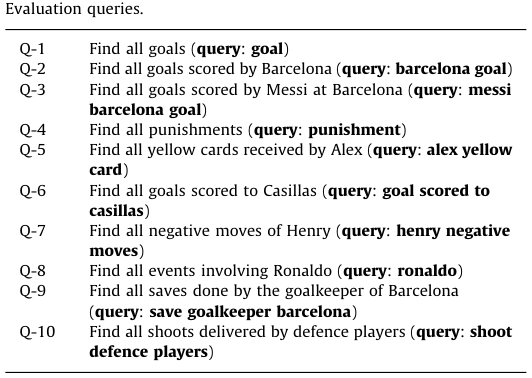
\includegraphics[width=3in]{fig/trans/tab3.png} 
	\caption[]{评价查询}
	\end{table} 

结果可以在表4中看到。首先,考虑前三个查询,{\Times TRAD}与其他方法就有了显著的区别。原因在于UEFA的解说中当{\Times P}得分了就用了短语“{\Times P}进了”。因为他省略了分这个字,在传统的索引中用关键词“得分”就不能检索出所有的进球。然而,信息解析模块能够成功地识别出进球,我们可以像文档那样在事件类型中给他填充为得分。因此,改善的索引就能响应“得分”和“进”这两种查询。这就是为什么{\Times BASIC\_EXT}和其他索引有非常高的查准率。
	\begin{table}[htbp] 
	\centering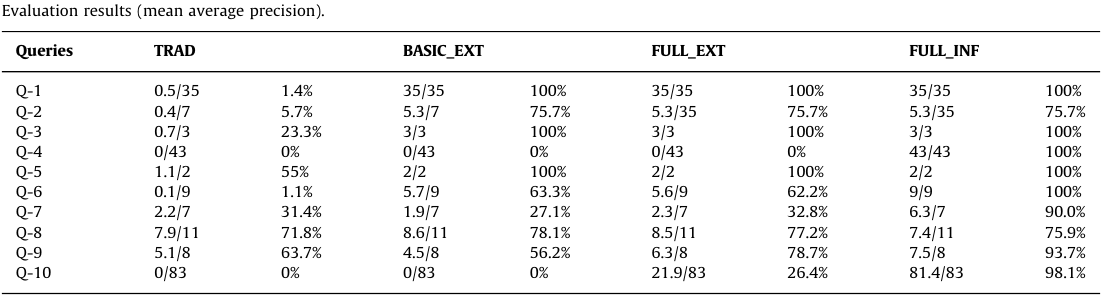
\includegraphics[width=6in]{fig/trans/tab4.png} 
	\caption[]{评价结果(平均查准率)}
	\end{table} 

这种能过信息解析模块产生的提高,可以通过{\Times BASIC\_EXT}和{\Times FULL\_EXT}中第9个和第10个的区别很容易看出来。这种区别源于解析射门和守门员扑救等事件。

这种提高源于推理,从查询4,7,10中很容易可以观察到。在这些查询中,{\Times FULL\_INF}索引表现得就比其他索引都要好,因为它包含了源于本体推理和分类的补充信息。例如,第4个查询提示了关于红牌和黄牌都是一种惩罚的推理知识。相似地,第10个查询则得益于通过分类推断出防守队员。最后,第7个查询用了定义于本体中的属性树的知识。这就意味着,系统可以识别属性,比如错过得分,越位和红牌,消极移动等。此外,在第6个查询中,我们可以看到{\Times Jena}规则的效果。在这儿,根据我们定义的规则之一,我们可以推断出精确的知识,比如哪次射门时是谁在守门,甚至并没有明确存在的知识。

如果我们看看查询8,就能发现四个索引效果并不多。原因在于,这是一个用单独的球员名字进行的简单搜索。所以,它并不包含太多语义索引可以利用的信息。然而,即使在这样的查询中,其性能也没有低于传统方法,因为全文的解说并没有被丢弃,而是保存在了一个独立的域中。换句话说,我们的方法保证了在最坏的情况下,也能与传统搜索一样。

我们的评估显示从{\Times BASIC\_EXT}开始,每一种索引都比它的前者有着显著的提高,而且最后在{\Times FULL\_INF}中,我们也达到了预期的效果。{\Times BASIC\_EXT}和{\Times FULL} {\Times \_EXT} 的性能也是让人满意的。在{\Times TRAD}和{\Times BASIC\_EXT}这间有明显的差别,因为它表现出即使是爬虫数据提供的基本信息,也会产生很大的不同。然而,当查询越来越复杂,我们需要具体的领域信息解析规则和推理来控制他们。所以,用这个框架,我们给开发者提供这样的机会,使他们可以根据用户的需要定制他们的系统。在任何情况下,这种框架都保证了提供可扩展性和用户友好性。

5.与查询扩展的比较

在第4部分,我们比较了我们的解决方法和传统方法,并看到了明显的提示不。然而,有人可能会问会不会出现这样的情况,只用扩展查询的方法就能达到之前的结果。因此,最后一个实验就展示了我们的解决方法和扩展查询方法的差异。为了填补这项空白,我们给用领域术语建的查询实现了一种原型,以此来扩展查询。例如,一个查询包含了“进球”将会扩展出动词“得分”,“错失”和其他派生词。本体信息也将被用在查询扩展中,因此,一个惩罚的查询将会被扩展到它的子类,比如“黄牌”“红牌”和动词“出牌”及其派生词。扩展查询直接在自由文本中运行,所以我们能清楚地看到查询扩展的提高,并能与我们的解决方案进行比较。

实验结果如表5所示。只要看一下,我们就能轻易地发现扩展查询的性能介于传统方法和语义索引,恰如我们所预料的那样。通过看查询1、2、3、4,我们能看到扩展查询的效果。前三个查询因为有了“得分”这个扩展,结果得以改善。在查询4中,因为有了惩罚这个术语的本体扩展,查询结果有了显著的提升。但是,性能依旧不如我们的本体索引法。因为没有合适的扩展术语,其他的查询结果没有受太大影响。对于一些搜索,这种搜索甚至会让结果更糟,因为它并不能正确捕捉到查询词汇的确切语义。
	\begin{table}[htbp] 
	\centering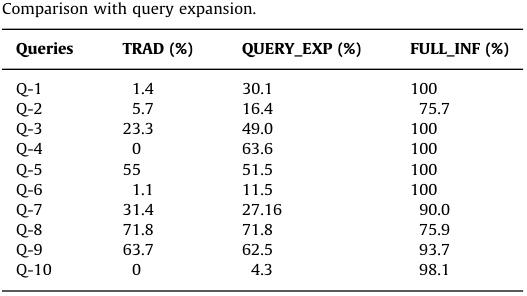
\includegraphics[width=3in]{fig/trans/tab5.png} 
	\caption[]{与查询扩展的比较}
	\end{table} 

6.增加短语支持

我们在3.6中提到了,关键词接口的搜索中最重要的问题是解决歧义。歧义出现通常有两种情况:词汇性的和结构性的。词汇性歧义由同义词导致,而结构性歧义由一词多义导致。只有信息扩展模块能够识别出词汇的歧义,我们才能解决,而我们并不没有实现一种词汇消除歧义的方法。然而,结构性歧义在关键词索引阶段就可以被解决。为了证明这一点,我们通过在现有系统上增加短语表达支持就解决了简单的结构性歧义问题。

假设一个用户想要查询{\Times Alex}对{\Times Ronaldo}的犯规,他会输入一个查询”犯规 {\Times Alex Ronaldo}”。系统可能会检索出{\Times Ronaldo}对{\Times Alex}的犯规,因为两个对员都可能犯规。为了解决这种结构性的歧义,我们引入了一些简单的短语表达,比如“对某人”,“被某人”,“属于某人”等,这样一来,系统就能知识查询对象是主体还是客体。这种实现的开销是微不足道的,因为只要填加了两个域,一个给主语,一个给宾语就可以实现了。每一个域的内容,都会有相应的介词与主语或是宾语相连。

我们对原始的版本({\Times FULL\_INF})和新的索引({\Times PHR\_EXP})做了比较。为此,我们做了三个人工查询。第一个查询测量主语混淆的性能({\Times Daniel}是制造犯规的人)。第二个查询往第一个中增加一个宾语({\Times Florent}),最后在第三种查询中,调换主宾的位置。结果见表6。注意到原来的索引在把握歧义的问题上遇到了困难,它并不能识别出谁是动作的主语,谁是宾语,但却不知道什么原因的,一直把{\Times Florent}当成了动作的主语。从另一方面来说,新的索引在任何条件下都能区分主语和宾语。
	\begin{table}[htbp] 
	\centering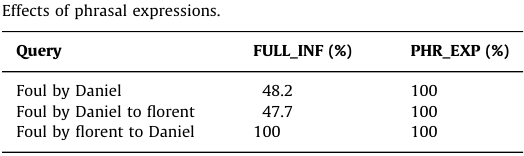
\includegraphics[width=3in]{fig/trans/tab6.png} 
	\caption[]{短语表达的影响}
	\end{table} 

7.讨论

本文展示了怎么样在保证了可扩展性和用户友好性的前提下,达到语义查询效果的。我们的方法还有另一个优势,那就是灵活性,尽管我们在研究中没有含盖,也就是说系统能够很容易的升级数据或是作出修改。我们认为用语义索引作为本体的上层,能够让基础知识变得更加灵活。

今天,大多数的语义应用都是以本体作为系统的主要数据结构,也就是说,要对本体的实例直接进行繁重的读写操作。然后,本体和本体实例都不是被用在这样的条件下的。从定义来看,他们是很严格的,是知识和声明的一种正式的代表。换言之,它们是永恒的,并不能这么随便改变更新。因此对于这些任务,我们推荐用另一种存储数据的方式,比如我们方案所用到的语义索引。

为了证明语义索引的灵活性,我们给出下面这个例子。假设我们想在查询接口中增加其他的语言,这样我们就能用两种语言来查询基础知识了。为了用本体实例达到这个目的,就必须要给第二语言复制实例和带有转换值的属性。在本体很庞大的时候,任何一种方案都是不实际的。但是,通过语义索引,要给每个域增加翻译过的值就非常容易。用语义网同义词,自然语言短语,甚至是词干来扩展索引的术语,都能被证明用语义索引是很容易就实现的。

8.结论和未来的工作

我们提出了一种新颖的语义检索框架,并应用足球领域,它含盖了语义网的各个方面,包括本体发展,信息抽取,本体构建,推理,语义规则,语义索引和检索。当这些技术被整合在关键词搜索的界面中,我们就获得了一种友好的,高性能的,可扩展的语义检索系统。评估结果显示,我们的方法超过了扩展查询或是传统的方法。此外,我们注意到我们的系统不用{\Times SPARQL}这样的正式的查询语句就可以实现复杂的语义性搜索。

我们注意到系统性能可于{\Times SPARQL}相媲美,而它恰是语义性搜索的最佳工具。最后,我们展示如何用语义索引来解决歧义的问题。

现在的工作可以在多方面进行扩展和改善。首先,我们准备丰富基础知识,来实现第7部分所提到的多语言支持。通过引入消除一词多义模块,我们的性能也会有很大提升。最后,我们未来的目标这一就是要设计这样一种机制,能根据用户反馈自动地扩展索引。



\vspace{20pt}
\centering 书面翻译对应的原文索引
\vspace{9pt}

\noindent
{\Times \wuhao \setlength{\baselineskip}{17pt}
Kara, S., Alan, Ö., Sabuncu, O., Akpınar, S., Cicekli, N. K., \& Alpaslan, F. N. (2012). An ontology-based retrieval system using semantic indexing. Information Systems, 37(4), 294-305.
}


\end{document}
